\documentclass[10pt,titlepage,a4paper]{report} %twoside

% add Unicode support and use English as language
\usepackage[utf8]{inputenc}
\usepackage[english]{babel}

\title{Deep Algorithmic Trading}
\date{\today}
\author{Jaron Matzinger}
\raggedbottom
\flushbottom

% Pageformat and Styles
\usepackage{fancyhdr}
\usepackage{multicol}
\usepackage{array,etoolbox}
\usepackage{lscape}

% Use Helvetica as font
\usepackage[scaled]{helvet}
\renewcommand\familydefault{\sfdefault}
\usepackage[T1]{fontenc}

% Tables and inputs
\usepackage{longtable}
\usepackage{tabularx}
\usepackage{multirow}
\usepackage{rotating}
\usepackage{float}
\restylefloat{table}
\usepackage{colortbl}
\usepackage{numprint}
%\npthousandsep{'}
\npthousandsep{,}
\npdecimalsign{.}
\usepackage{siunitx}
\newcommand\dsh{\multicolumn{3}{c@{\hspace{2em}}}{--}}

% Citations
\usepackage{natbib}

\usepackage[utf8]{inputenc}

% Math tools
\usepackage{mathtools}
\usepackage{amssymb}
\usepackage{amsmath}
\usepackage{amsthm}
\usepackage{bbm}

% PDF include
\usepackage{pdfpages}

% CSV include
\usepackage{csvsimple}
\usepackage{booktabs}

\usepackage{tablefootnote}

\usepackage{textgreek}
\usepackage{flafter}
\usepackage[hidelinks]{hyperref}
\usepackage[normalem]{ulem}
\usepackage[colorinlistoftodos,prependcaption,textsize=tiny]{todonotes}

\usepackage{pifont}
\newcommand{\cmark}{\ding{51}}%
\newcommand{\xmark}{\ding{55}}%

\usepackage{footnote}
\makesavenoteenv{tabular}
\makesavenoteenv{table}

%%%%%%%%%%%
% Tikz to crate diagrams, thanks to: https://github.com/mvoelk/nn_graphics
% Start of tikz settings
\usepackage{dirtree}
\usepackage{tikz}
\usetikzlibrary{positioning,arrows.meta}
\usetikzlibrary{matrix, chains, positioning, decorations.pathreplacing, arrows}
\usetikzlibrary{shapes,arrows,positioning,calc,chains,scopes}

\usepackage{ifthen}
\usepackage{pgfplots}
\pgfplotsset{compat=1.15}
\pgfplotsset{every axis/.append style={tick label style={/pgf/number format/fixed},font=\scriptsize,ylabel near ticks,xlabel near ticks,grid=major}}

\usepackage{amsmath}
\DeclareMathOperator{\sigm}{sigm}
\newcommand{\diff}{\mathop{}\!\mathrm{d}}

% colors
\definecolor{snowymint}{HTML}{E3F8D1}
\definecolor{wepeep}{HTML}{FAD2D2}
\definecolor{portafino}{HTML}{F5EE9D}
\definecolor{plum}{HTML}{DCACEF}
\definecolor{sail}{HTML}{A3CEEE}
\definecolor{highland}{HTML}{6D885A}

\tikzstyle{signal}=[arrows={-latex},draw=black,line width=1pt,rounded corners=4pt]

% RNN
\tikzstyle{block}=[draw=black,line width=1.0pt]
\tikzstyle{cell}=[style=block,draw=highland,fill=snowymint,
    rounded corners]
\tikzstyle{celllayer}=[style=block,draw,fill=portafino,
    inner sep=1pt,outer sep=0,
    minimum width=28pt, minimum height=14pt]
\tikzstyle{pointwise}=[style=block,ellipse,fill=wepeep,
    inner sep=1pt,outer sep=0, minimum size=12pt]

\def\iolen{24pt}
\def\intergape{2pt}

% MLP and CNN
\tikzstyle{netnode}=[circle, inner sep=0pt, text width=22pt, align=center, line width=1.0pt]
\tikzstyle{inputnode}=[netnode, fill=sail, draw=black]
\tikzstyle{hiddennode}=[netnode, fill=snowymint, draw=black]
\tikzstyle{infonode}=[netnode, fill=portafino, draw=black, inner sep=6pt, font=\Large]
\tikzstyle{outputnode}=[netnode, fill=plum, draw=black]

% Architecture
\def\layerwidth{120pt}
\def\layerheight{30pt}

\tikzstyle{layer}=[style=block, draw, fill=black!20!white,
    inner sep=5pt,outer sep=0pt, font=\footnotesize,
    text centered, align=center,
    minimum width=\layerwidth, minimum height=\layerheight]

\tikzstyle{fc}=[style=layer, fill=blue!30!white]
\tikzstyle{conv}=[style=layer, fill=green!30!white]
\tikzstyle{activation}=[style=layer, fill=orange!30!white]
\tikzstyle{pool}=[style=layer, fill=red!30!white]
\tikzstyle{bn}=[style=layer, fill=cyan!30!white]
\tikzstyle{recurrent}=[style=layer, fill=purple!30!white]
\tikzstyle{softmax}=[style=layer, fill=yellow!30!white]
\tikzstyle{point}=[]
\tikzstyle{branch}=[coordinate]

\def\vlayerwidth{30pt}
\def\vlayerheight{3pt}
\def\vblockheight{28pt}

\tikzstyle{vlayer}=[minimum width=\vlayerwidth, minimum height=\vlayerheight]
\tikzstyle{vblock}=[minimum width=\vlayerwidth, minimum height=\vblockheight, text width=1cm, align=center]

% Precision, Recall
\colorlet{fn}{gray!90!green!30!white}
\colorlet{tp}{green!40!white}
\colorlet{fp}{red!40!white}
\colorlet{tn}{gray!90!red!20!white}
% End of tikz settings
%%%%%%%%%%%

\setlength{\columnsep}{0.5cm}

%%%%%%%%%%%%%%%%%%%%%%%%%%%%
% Graphics, plots and figures
\usepackage{pgfplots}
\pgfplotsset{compat=newest,compat/show suggested version=true}
\usepackage{tikz}
\usetikzlibrary{shapes.geometric, arrows, decorations.pathreplacing,matrix,shapes,positioning,chains}
\newcommand*\circled[1]{\tikz[baseline=(char.base)]{
		\node[shape=circle,draw,inner sep=0.4pt] (char) {#1};}}
\newcommand*\ellipsed[1]{\tikz[baseline=(char.base)]{
		\node[shape=ellipse,draw,inner sep=0.4pt] (char) {#1};}}
\usepackage{graphicx}
\usepackage{caption}
\usepackage{subcaption}
\newenvironment{Figure}
{\par\medskip\noindent\minipage{\linewidth}}
{\endminipage\par\medskip}
\usepackage[export]{adjustbox}

\usepackage{makeidx}
\usetikzlibrary{calc}
\newcommand{\tikzmark}[1]{\tikz[baseline,remember picture] \coordinate (#1) {};}

\newcounter{magicrownumbers}
\newcommand\rownumber{\stepcounter{magicrownumbers}\arabic{magicrownumbers}}

% Algorithms
\usepackage{algorithm} 
\usepackage{algorithmic}  
\usepackage[algo2e]{algorithm2e} 
\newcommand{\assign}{$\leftarrow$}
% Python style
\SetStartEndCondition{ }{}{}%
\SetKwProg{Fn}{def}{\string:}{}
\SetKwFunction{Range}{range}%%
\SetKw{KwTo}{in}\SetKwFor{For}{for}{\string:}{}%
\SetKwIF{If}{ElseIf}{Else}{if}{:}{elif}{else:}{}%
\SetKwFor{While}{while}{:}{}%

\usepackage{listings}
\lstset{
	frame=single,
	breaklines=true,
	postbreak=\raisebox{0ex}[0ex][0ex]{\ensuremath{\color{red}\hookrightarrow\space}},
	backgroundcolor=\color[rgb]{0.95,0.95,0.95},
}

% Acronym definitions
\usepackage[acronym]{glossaries}
\loadglsentries{acronyms}
\glsdisablehyper
\makeglossaries

% Page Settings
\usepackage[top=26mm,bottom=26mm,left=23mm,right=31mm]{geometry}

\pagestyle{fancy}
\fancyhf{}
\renewcommand{\headrulewidth}{0pt}
\renewcommand{\footrulewidth}{0pt}
\fancypagestyle{beginning}{
	\fancyhf{}
	%\fancyfoot[RO,LE]{\normalsize\thepage}
	\pagenumbering{Roman}% Roman-numbered pages (start from i)
	\renewcommand{\headrulewidth}{0pt}
	\renewcommand{\footrulewidth}{0pt}
}

\fancypagestyle{normal}{
	\fancyhf{}
	%\fancyhead[CE,CO]{\leftmark}
	%\fancyfoot[RO,LE]{\thepage}
	%\fancyhead[LO,RE]{\leftmark}
 	\fancyhead[C]{\leftmark} % Centered header
	\fancyfoot[C]{\thepage} % Centered footer
	%\fancyfoot[C]{}
	\pagenumbering{arabic}
	\renewcommand{\headrulewidth}{0pt}
	\renewcommand{\footrulewidth}{0pt}
}
% Redefine the plain page style
\fancypagestyle{plain}{%
	\fancyhf{}%
	\cfoot{\thepage}
        %\fancyfoot[RO,LE]{\thepage}
	\renewcommand{\headrulewidth}{0pt}% Line at the header invisible
	\renewcommand{\footrulewidth}{0pt}% Line at the footer visible
}

\usepackage{titlesec}
\makeatletter
\renewcommand{\@makeschapterhead}[1]{%
	%  \vspace*{50\p@}%
	\vspace*{20\p@}%
	{\parindent \z@ \raggedright
		\normalfont
		\interlinepenalty\@M
		\Huge \bfseries  #1\par\nobreak
		%    \vskip 40\p@
		\vskip 20\p@
}}
\makeatother

% Formulas
\newcommand{\rulesep}{\unskip\ \vrule\ }
\newcommand{\empt}[2]{$#1^{\langle #2 \rangle}$}
\renewcommand{\vec}[1]{\boldsymbol{\mathbf{#1}}}
\def \h {\vec{h}}
\def \y {\vec{y}}
\def \x {\vec{x}}
\def \W {\vec{W}}
\def \b {\vec{b}}
\def \realnumbers {\mathbb{R}}
\DeclarePairedDelimiter\ceil{\lceil}{\rceil}
\DeclarePairedDelimiter\floor{\lfloor}{\rfloor}
\newcommand{\norm}[1]{\left\lVert #1 \right\rVert}

% Need a list of equation
\usepackage{tocloft}
\usepackage{ragged2e}
% Define list of equations - Thanks to Charles Clayton: https://tex.stackexchange.com/a/354096
\newcommand{\listequationsname}{List of Equations}
\newlistof{myequations}{equ}{\listequationsname}
\newcommand{\myequations}[1]{
	\addcontentsline{equ}{myequations}{\protect\numberline{\theequation}#1}
}
\setlength{\cftmyequationsnumwidth}{2.3em}
\setlength{\cftmyequationsindent}{1.5em}

% equations with term definitions, credit to tex.stackexchange.com/questions/95838/how-to-write-a-perfect-equation-parameters-description
\newenvironment{conditions}
  {\par\vspace{\abovedisplayskip}\noindent\begin{tabular}{>{$}l<{$} @{${}={}$} l}}
  {\end{tabular}\par\vspace{\belowdisplayskip}}
  
\newenvironment{conditions*}
  {\par\vspace{\abovedisplayskip}\noindent
   \tabularx{\columnwidth}{>{$}l<{$} @{${}={}$} >{\raggedright\arraybackslash}X}}
  {\endtabularx\par\vspace{\belowdisplayskip}}
%%%%%%%%%%%%%%%%%%%%%%%%%%%%%%%%%%%%%%%%%%%%%%%%%%
%% Example Environment:
%%%%%%%%%%%%%%%%%%%%%%%%%%%%%%%%%%%%%%%%%%%%%%%%%%

\newtheorem{exmpl}{Example}[chapter]
\newenvironment{example} 
{\begin{exmpl}}
	{\nopagebreak\hfill\mbox{$\ominus$}\end{exmpl}}

% Acronyms
\makeindex

\begin{document}
	\pagenumbering{gobble}
	%%%%%%%%%%%%%%%%%%%%%%%%%%%%%%%%%%%%%%%%%%%%%%%%%%%%%%%%%%%%%%
	% Title
	\begin{titlepage}
    \centering
    {\small\text{\ }\par}
    \vspace{2cm}
    {\huge\bfseries 
    Deep Algorithmic Trading
    \par}
    \vspace{4cm}
    {\large\text Bachelor of Science in Artificial Intelligence \& Machine Learning \par
    \scshape\Large{Bachelor Thesis}\par
    }
    \vspace{1cm}
    {\large\text{presented by}\par
        \scshape\Large Jaron Matzinger\par}
    \vspace{1cm}
    {\large\text{Department of Computer Science and Information Technology} \par
        \large\text{Lucerne University of Applied Sciences and Arts} \par
        \large\text{6343 Rotkreuz, Switzerland} \par}
    
    \vspace{4cm}
    {\large \today\par}
    \vfill
    \begin{tabular}[t]{l l}
            Advisor & 
            Fabian Gröger \\
            & Lucerne University of Applied Sciences and Arts, 6343 Rotkreuz, Switzerland \\
            & fabian.groeger@hslu.ch \\
            & \\
            
            Expert &
            Dr.\ Stefan Egle \\
            & Lorem Ipsum, Switzerland \\
            & stefan.egle@lorem\_ipsum.com \\
    
    \end{tabular}
    \vfill

    \clearpage

    \begin{flushleft}
        \vspace{2cm}
        {\Large \textbf{Bachelor Thesis at Lucerne University of Applied Sciences and Arts School of Computer Science and Information Technology} \par}
        \vspace{2cm}
        
        \begin{tabular}{@{}ll}
            \vspace{0.5cm}
            \large \textbf{Title of Bachelor Thesis:}  & 
            \large Deep Algorithmic Trading \\
            \vspace{0.5cm}
            \large \textbf{Name of Student:} &
            \large Jaron Matzinger \\
            \vspace{0.5cm}
            \large \textbf{Degree Program:} &
            \large BSc AIML \\
            \vspace{0.5cm}
            \large \textbf{Year of Graduation:} &
            \large 2024 \\
            \vspace{0.5cm}
            \large \textbf{Main Advisor:} &
            \large Fabian Gröger \\
            \vspace{0.5cm}
            \large \textbf{External Expert:} &
            \large Stefan Egle \\
            \vspace{0.5cm}
            \large \textbf{Industry Partner:} &
            \large MP Venverse AG \\
        \end{tabular}

        \vspace{1.0cm}
        \large \textbf{Code / Thesis Classification:} \\
        $\square$ Public (Standard) \\
        $\square$ Private \\
        \vspace{1.5cm}
        \textbf{Declaration} \\
        I hereby declare that I have completed this thesis alone and without any unauthorized or external help. I further declare that all the sources, references, literature, and any other associated resources have been correctly and appropriately cited and referenced. The confidentiality of the project provider (industry partner) as well as the intellectual property rights of the Lucerne University of Applied Sciences and Arts have been fully and entirely respected in the completion of this thesis. \\
        \vspace{0.5cm}
        \textbf{Place / Date, Signature} \quad \rule{10.5cm}{0.4pt} \\
        \vspace{1.5cm}
        \textbf{Submission of the Thesis to the Portfolio Database:} \\
        Confirmation by the student \\
        I hereby confirm that this bachelor thesis has been correctly uploaded to the Portfolio Database in line with the code of practice of the University. I rescind all responsibility and authorization after upload so that no changes or amendments to the document may be undertaken. \\
        \vspace{0.5cm}
        \textbf{Place / Date, Signature} \quad \rule{10.5cm}{0.4pt} 
    \end{flushleft}

    \clearpage
    \mbox{}
    \vfill
    \begin{flushleft}
    
    \noindent
    \textbf{Acknowledgements.\ }I want to thank my advisor Fabian Gröger, for the great discussions and support during the thesis.\ Furthermore, I appreciate the interesting exchange with Stefan Egle from XYZ AG as well as the support and guidance offered by Pascal Baumann. Finally, I would like to express my deepest appreciation to my girlfriend, Linda Leuenberger, for her continuous support during this thesis.\
    \newline
    \newline
    \textbf{Use of LLMs.\ } During the writing process of this thesis, I used large language models (LLMs) to improve the text, rephrase content, and find synonyms. However, to preserve the original meaning, the outputs from these tools were always carefully reviewed.
    \newline
    \newline
    \textbf{Inspiration for Theoretical Grounding chapter.\ } The content and especially the structure of chapter 2 was influenced by previous research conducted by Fabian Gröger.
    \newline
    \newline
    \textbf{Declaration of originality.\ }I hereby declare that I have prepared the present work independently and have used nothing other than the specified aids.\ All text sections, citations or contents of other authors used have been explicitly marked as such.\ 

    \vspace{0.25cm}
    \begin{center}
        
\includegraphics[scale=0.3]{assets/img/unterschrift.png} \\
        Zürich \\ 
        \today \\ 
        Jaron Matzinger
    \end{center}
    \vspace{0.75cm}
    
    \textit{Intellectual property of the degree programs of the Lucerne University of Applied Sciences and Arts, FH Zentralschweiz, in accordance with Student Regulations: \href{https://srl.lu.ch/app/de/texts_of_law/521/versions/4065}{Studienordnung}}

    \end{flushleft}

\end{titlepage}
	
\clearpage
	\pagestyle{beginning}
	%%%%%%%%%%%%%%%%%%%%%%%%%%%%%%%%%%%%%%%%%%%%%%%%%%%%%%%%%%%%%
	% Abstract
	\chapter*{Abstract}
% introduction
	\newpage
		
	%%%%%%%%%%%%%%%%%%%%%%%%%%%%%%%%%%%%%%%%%%%%%%%%%%%%%%%%%%%%%
	% Table of Content
	\tableofcontents
	\newpage
	
	%%%%%%%%%%%%%%%%%%%%%%%%%%%%%%%%%%%%%%%%%%%%%%%%%%%%%%%%%%%%%
	% Start with numbering
	\pagestyle{normal}
	
	\chapter{Introduction}
\label{ch:Introduction}
This chapter introduces the bacholor thesis's problem and derived objective.

\section{Initial Situation \& Problem}
\label{sec:InitialSituation}
In 1970, Eugene Fama introduced the \gls{emh}, which argues that publicly available information does not allow investors to consistently outperform a global benchmark such as the S\&P500 \citep{fama1970efficient}. In 1988, Halbert White attempted to find empirical evidence against the \gls{emh} by using an \gls{ann} to predict IBM's daily stock returns. He was unable to find convincing statistical evidence against it \citep{white1988economic}, thereby supporting Fama's hypothesis.
\newline
\newline
Undeterred, major financial institutions such as Bloomberg have devoted significant resources to achieving alpha, which essentially means outperforming the market. Machine learning plays a pivotal role in this endeavour, encompassing tasks such as sentiment analysis and named entity recognition \citep{wu2023bloomberggpt}.
\newline
\newline
Alongside these established institutions, new entrants have joined the hunt for alpha. Neo-brokers such as Robinhood have democratised financial services and as a result have seen significant user growth in recent years, as shown in figure \ref{fig:users_RH}. However, it's worth noting that the average Robinhood trader has failed to outperform the S\&P 500 index \citep{canellis-2020}, in line with the \gls{emh}.

\begin{figure}[ht]
    \centering
    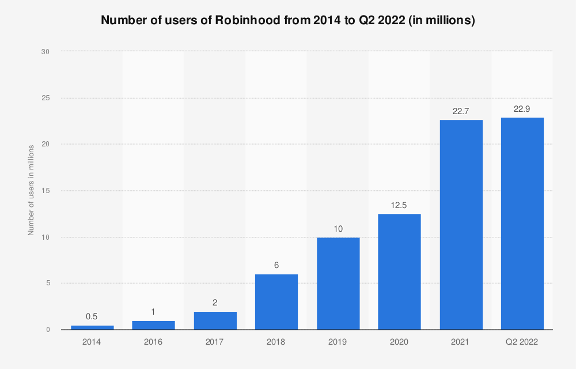
\includegraphics[width=0.85\textwidth]{./assets/img/users_rh.png}
    \caption{Figure shows the number of users on Robinhood from 2014 to Q1 2022. Figure from \cite{statista_robinhood}.}
    \label{fig:users_RH}
\end{figure}

\clearpage
\noindent
This raises a fascinating question: If researchers like White cannot find empirical evidence against the \gls{emh}, and the average Robinhood trader is also not able to beat a global benchmark like the S\&P500, why are financial institutions still trying to achieve alpha by processing financial data with machine learning models?

\section{Research Objective}
\label{sec:ResearchObjective}
This empirical research project aims to train several machine learning models on historical cryptocurrency price and volume data, and evaluate their performance against well-known momentum indicators as baselines and a global benchmark.
	\chapter{Theoretical Grounding}
\label{ch:TheoreticalGrounding}
This chapter introduces and explains terms and concepts relevant for this thesis. In order to follow the empirical research throughout the thesis, it is important to gain fundamental knowledge in the domains of financial markets, technical analysis, and machine learning.

\section{Financial Markets}
\label{sec:FinMarket}
Financial markets comprise of various concepts, terms and instruments. This section delves into the these aspects and elaborates on them.

\subsection{Cryptocurrencies}
\label{sub:crypto}
A segment of the financial markets is cryptocurrencies, a specific type of digital assets that mostly operates within a \gls{p2p} network called a blockchain. The blockchain usually consists of the \gls{dlt} and a consensus mechanism. The \gls{dlt} operates through a network of interconnected nodes that collectively maintain and verify transaction records. In the context of well-known cryptocurrencies such as \gls{btc} \citep{bitcoin_2008}, the consensus protocol used is known as proof-of-work, in which participating nodes must solve complex cryptographic puzzles to validate transactions and add a new block to the chain in exchange for a reward. This process involves the broadcast of the newly added block to ensure a unique, immutable chain throughout the network. The following terms are used throughout this thesis.

\begin{description}
    \item[\gls{btc}] is the world's first and most popular cryptocurrency. \gls{btc} was introduced in 2008 by an anonymous person or group of people using the pseudonym Satoshi Nakamoto.
    \item[\gls{eth}] is the second largest and most popular cryptocurrency. It was introduced in 2014 by Vitalik Buterin \citep{eth_2014}. Buterin integrated smart contracts into the blockchain framework. These smart contracts allow transactions to be executed through predetermined, immutable algorithms stored on the blockchain, effectively eliminating the need for any type of intermediary.
    \item[Alternative coins,] or more commonly referred to as altcoins or alts, encompass all cryptocurrencies other than \gls{btc}. While \gls{eth} technically falls into the altcoin category, its profound impact and prolonged presence, spanning nearly nine years, has led some to view it as a prominent entity akin to \gls{btc} itself.
\end{description}

\noindent
Next, some basic financial market terms applied to the cryptocurrency domain are introduced.

\subsection{Time Frames}
\label{sub:TF}
A \gls{tf} refers to a specific time interval used to analyse price data in financial markets. Commonly used \glspl{tf} are 1-minute, 15-minute, 1-hour, 4-hour, daily, weekly and monthly. This thesis will focuses primarily on the daily \gls{tf}.

\subsection{Open-High-Low-Close Price}
\label{sub:OHLC}
The \gls{ohlc} price is correlated to the selected \gls{tf}. Open is the price at the beginning of the \gls{tf} period. High is the highest price reached during the period. Low is the lowest price reached during the period and close is the price at the end of the period.
\newline
\newline
For example, if the \gls{tf} is set to daily, the open price will be the price at 00:00:00 and the close price will be the price at 23:59:59. During this period there will be a high and a low in the price. In the cryptocurrency space, these prices can be within a wide range. For example, the price of \gls{btc} may open at 00:00 with a price of \$20,000.00, then rise during the day to \$21,590.00, which signals the high, and then fall to \$19,200.00, which signals the low, and finally close at 23:59 at \$19,900.00.

\subsection{Volume}
\label{sub:volume}
Volume refers to the total number of units of an asset traded in a given \gls{tf}. It is a critical indicator in cryptocurrency markets as it provides insight into market activity and liquidity. High trading volumes can indicate increased market interest and potential price movements.

\subsection{Market Capitalization}
\label{sub:MarketCap}
Market capitalization, often referred to as market cap, is the total value of a cryptocurrency. It is calculated by multiplying a cryptocurrency's current market price by the total supply in circulation. Market cap is often used to rank and compare cryptocurrencies and is an indicator of their relative size within the market.

\subsection{Volatility}
\label{sub:Vola}
Volatility refers to the degree to which the price of an asset fluctuates over time. In the context of cryptocurrencies, high volatility means that prices can change rapidly and significantly in a short period of time, as discussed in section \ref{sub:OHLC}. Volatility can present both opportunities and risks for traders and investors.

\subsection{Exchanges}
\label{sub:Exchanges}
Exchanges are online platforms where users can buy and sell cryptocurrencies. They act as intermediaries that facilitate the exchange of digital assets. The most prominent exchange in the world is Binance, followed by Coinbase. There are several others such as Bybit and OKX.

\subsection{Bid-Ask Spread}
\label{sub:Bid-Ask}
The bid-ask spread is the difference between the highest price a buyer is willing to pay (the bid) and the lowest price a seller is willing to accept (the ask) for an asset. It represents the transaction cost to traders and reflects the liquidity of an asset. A tighter spread indicates a more liquid market.

\subsection{Market Maker}
\label{sub:MM}
The \glspl{mm} play a pivotal role in the financial markets, particularly in maintaining liquidity and managing the bid-ask spread. As explained in the previous section, they are specialized entities or individuals equipped to facilitate the trading of financial assets.
\newline
\newline
\glspl{mm} continuously provide both bid and ask prices for a specific asset. When they acquire an asset at the ask price, they don't immediately sell the same asset at the bid price. Instead, they execute trades with another unit of the identical asset that they acquired at a lower cost, matching the bid. This strategic approach allows \glspl{mm} to profit from the price differential between the bid and ask, while simultaneously ensuring that there is a continuous flow of buy and sell orders.
\newline
\newline
By providing liquidity and facilitating trading, \glspl{mm} help maintain market efficiency and encourage market participation. Their actions directly impact the bid-ask spreads, with narrower spreads indicating a more liquid and competitive market environment.

\subsection{Derivatives}
\label{sub:Derivatives}
Derivatives are financial instruments that derive their value from underlying assets, indices, or reference rates. In the cryptocurrency space, two of the most important types of derivatives are spot contracts and perpetual futures contracts.

\subsubsection{Spot Contract}
\label{subsub:Spot}
Spot, short for spot contract, allows one market participant to exchange the underlying asset directly with another market participant. In summary, spot facilitates the exchange of assets between two market participants through an exchange (see section \ref{sub:Exchanges}).

\subsubsection{Futures Contract}
\label{subsub:Futures}
A futures contract, often called a futures, gives market participants the option to buy the underlying asset in the future at the price at which the contract was sold. These contracts have a predetermined expiration date in the future, after which they become void. Futures are widely used in various sectors, including agriculture and finance.

\subsubsection{Perpetual Contract}
\label{subsub:Perps}
Perps, short for perpetual contracts, are a specialized type of futures primarily used in the cryptocurrency space. Unlike traditional futures, perps have no expiration date. They allow market participants to buy and sell assets without directly owning them. Perps are particularly important for shorting (see section \ref{sub:OrderTypes}), allowing traders to profit from declining asset prices.

\subsection{Order Types}
\label{sub:OrderTypes}
In general, there are two main types of orders: buy orders (referred to as long) and sell orders (referred to as short). These orders can be further categorized into different order types based on their timing. However, for the purposes of this thesis, only the two main types of orders will be considered: market and limit orders.

\subsubsection{Market Order}
\label{subsub:MarketOrder}
A market order is designed to execute a trade – either a buy or a sell – at the current market price. It prioritises the speed of execution of the order over the specific price at which the trade is executed. Market orders are used when traders want to execute a transaction immediately, regardless of the current market price.

\subsubsection{Limit Order}
\label{subsub:LimitOrder}
A limit order is designed to execute a trade – either a buy or a sell – at a pre-defined market price. It prioritises the specific price over the rapid execution of the order. Limit orders are used when traders want to execute a transaction at a specific price. It is possible that the desired price will never be reached and therefore the limit order will never be executed.

\newpage
\section{Technical Analysis}
\label{sec:TechnicalAnalysis}
Technical analysis covers a wide range of concepts, techniques and tools that help traders and investors analyse financial markets and make informed trading decisions based on historical price, volume and other related market data. In order to follow the thesis, it is important to gain a basic knowledge of technical indicators from the field of technical analysis.

\subsection{Technical Indicators}
\label{sec:TechnicalIndicators}

% Introduction
As James Chen of Investopedia puts it: ["Technical indicators are heuristic or pattern-based signals produced by the price, volume, and/or open interest of a security or contract used by traders who follow technical analysis"] \citep{Chen_2021}. These indicators are essential tools for traders and analysts to make informed decisions.
\newline
\newline
% The price chart
All technical indicators are applied to a price chart, which provides traders and investors a visual representation of historical price movements in financial markets. Price charts as illustrated in figure \ref{fig:bitcoin_price_chart}, offer insights into market trends, patterns and potential future price directions, enabling investors to make informed trading decisions. Common types of price charts include line charts, bar charts and candlestick charts, each offering a unique perspective on market dynamics. By incorporating technical indicators such as \gls{ma}, \gls{bb} and stochastic oscillators, traders can further analyse price chart patterns to identify potential entry and exit points, as well as gauge market momentum and volatility.

\begin{figure}[ht]
    \centering
    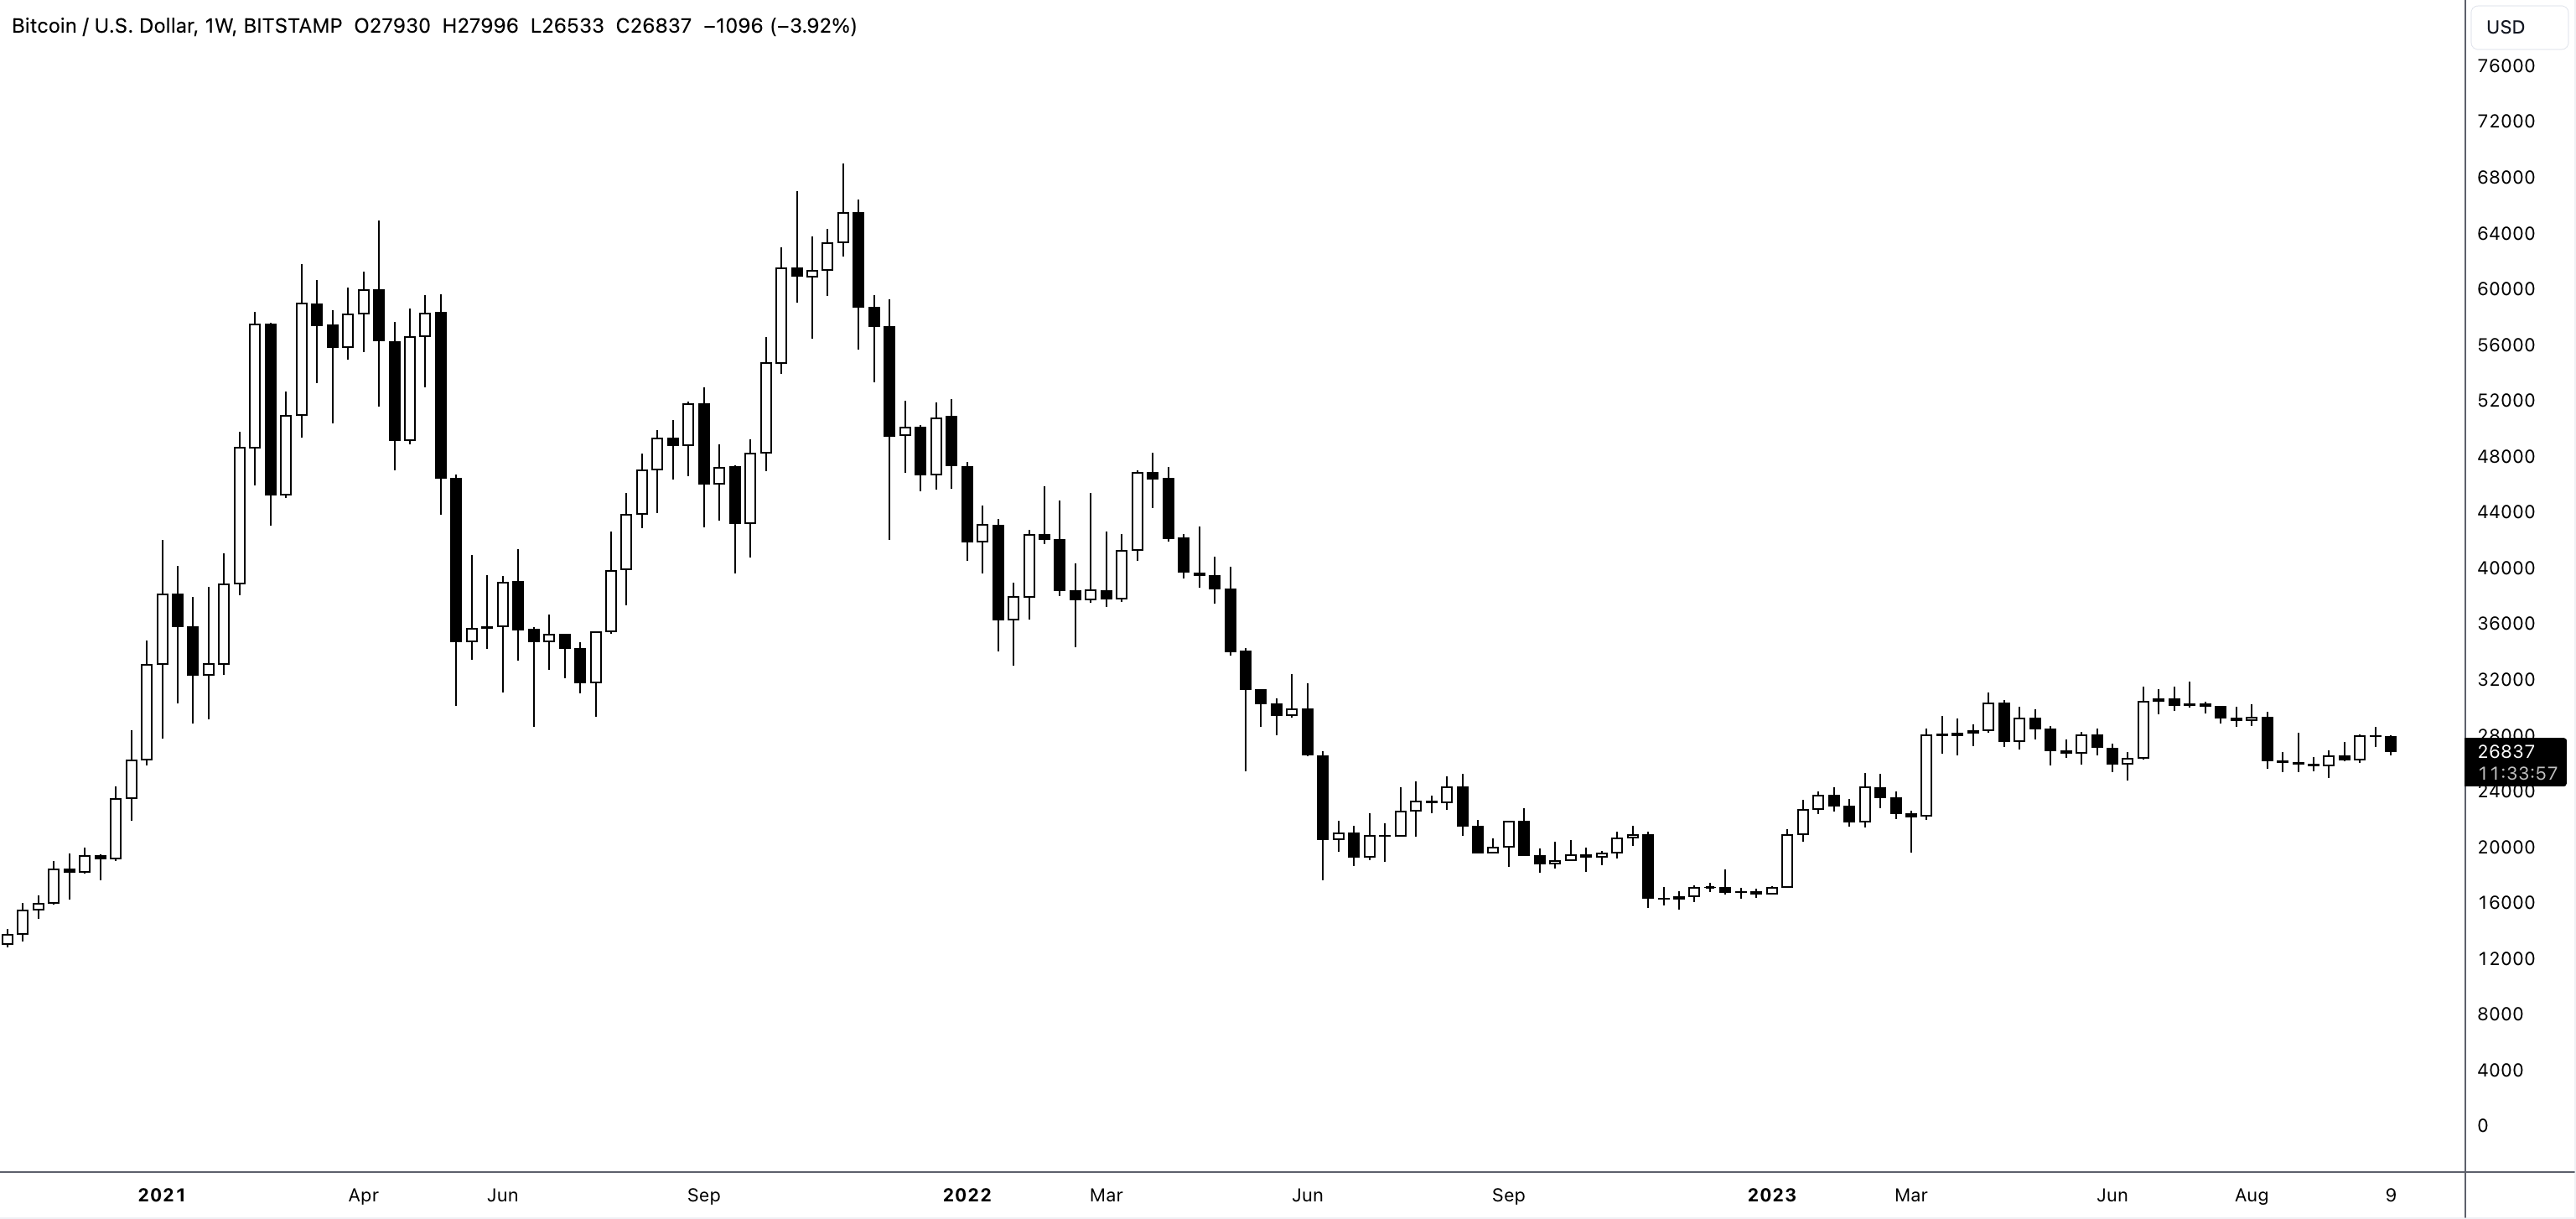
\includegraphics[width=\textwidth]{./assets/img/bitcoin_price_chart.png}
    \caption{Figure shows weekly price movements of \gls{btc} in USD as a candlestick chart from October 2020 to October 2023.}
    \label{fig:bitcoin_price_chart}
\end{figure}

\noindent
% Types of Technical Indicators
Technical indicators can be divided into two main types: momentum and lagging indicators. Momentum indicators measure the rise or fall of asset prices, helping to assess their current strength. On the other hand, lagging indicators signal market changes after they have already occurred, thus confirming the long-term trend.
\newline
\newline
Furthermore, both momentum and lagging can be further categorized into overlays and oscillators. Overlays are plottet on the price chart itself and have the same scale as the price. Examples of overlays are \gls{ma} and \gls{bb}. Oscillators, on the other hand, are indicators that osciallate between local minima and maxima and are typically plotted below the price chart. Well-known oscillators include the \gls{rsi} and the \gls{macd} \citep{Chen_2021}.

% Moving Average
\subsection{Moving Average}
\label{sub:MA}
The \gls{ma} is a technique for smoothing data points that has been used for decades, long before a general term came into use. In 1909, G. U. Yule \citep{yule1909applications} described the ["instantaneous averages"] of R. H. Hooker \citep{hooker1901correlation} as ["moving averages"]. But Yule did not adopt the term in his textbook. It came into circulation through W. I. King's book \textit{Elements of Statistical Method} in 1912 \citep{king1912elements}.
\newline
\newline
The \gls{ma} is a fundamental indicator used in technical analysis to smooth price data, reduce noise and highlight trends. Traders and investors commonly use the 50-day and 200-day \gls{ma} as important \glspl{tf} for analysis. The 50-day \gls{ma} looks at the past 50 trading days, while the 200-day \gls{ma} looks at the past 200 days. Because the \gls{ma} is based on historical price data, it is generally considered to be a lagging indicator.
\newline
\newline
There are two main types of \gls{ma}: the \gls{sma} and the \gls{ema}. The \gls{sma} calculates the arithmetic mean $\frac{1}{d}$ of the price $v_t$ over a specified time period from $t = 1, 2, \dots, d$, represented as $\text{SMA} = \frac{1}{d} \sum_{t=1}^d v_t$. On the other hand, the \gls{ema} integrates a smoothing factor $k$ to give greater weight to recent prices within the time period $d$. The calculation of the \gls{ema} can be expressed as in the equation \ref{eq:exp_moving_average}, where $k$ is denoted as $\frac{2}{d + 1}$.

\myequations{Computing the exponential moving average}
\begin{equation}
    \centering
    \text{EMA}_t =  v_t \cdot k + \text{SMA}_{t-1} \cdot (1 - k) 
    \label{eq:exp_moving_average}
\end{equation}

\begin{figure}[ht]
    \centering
    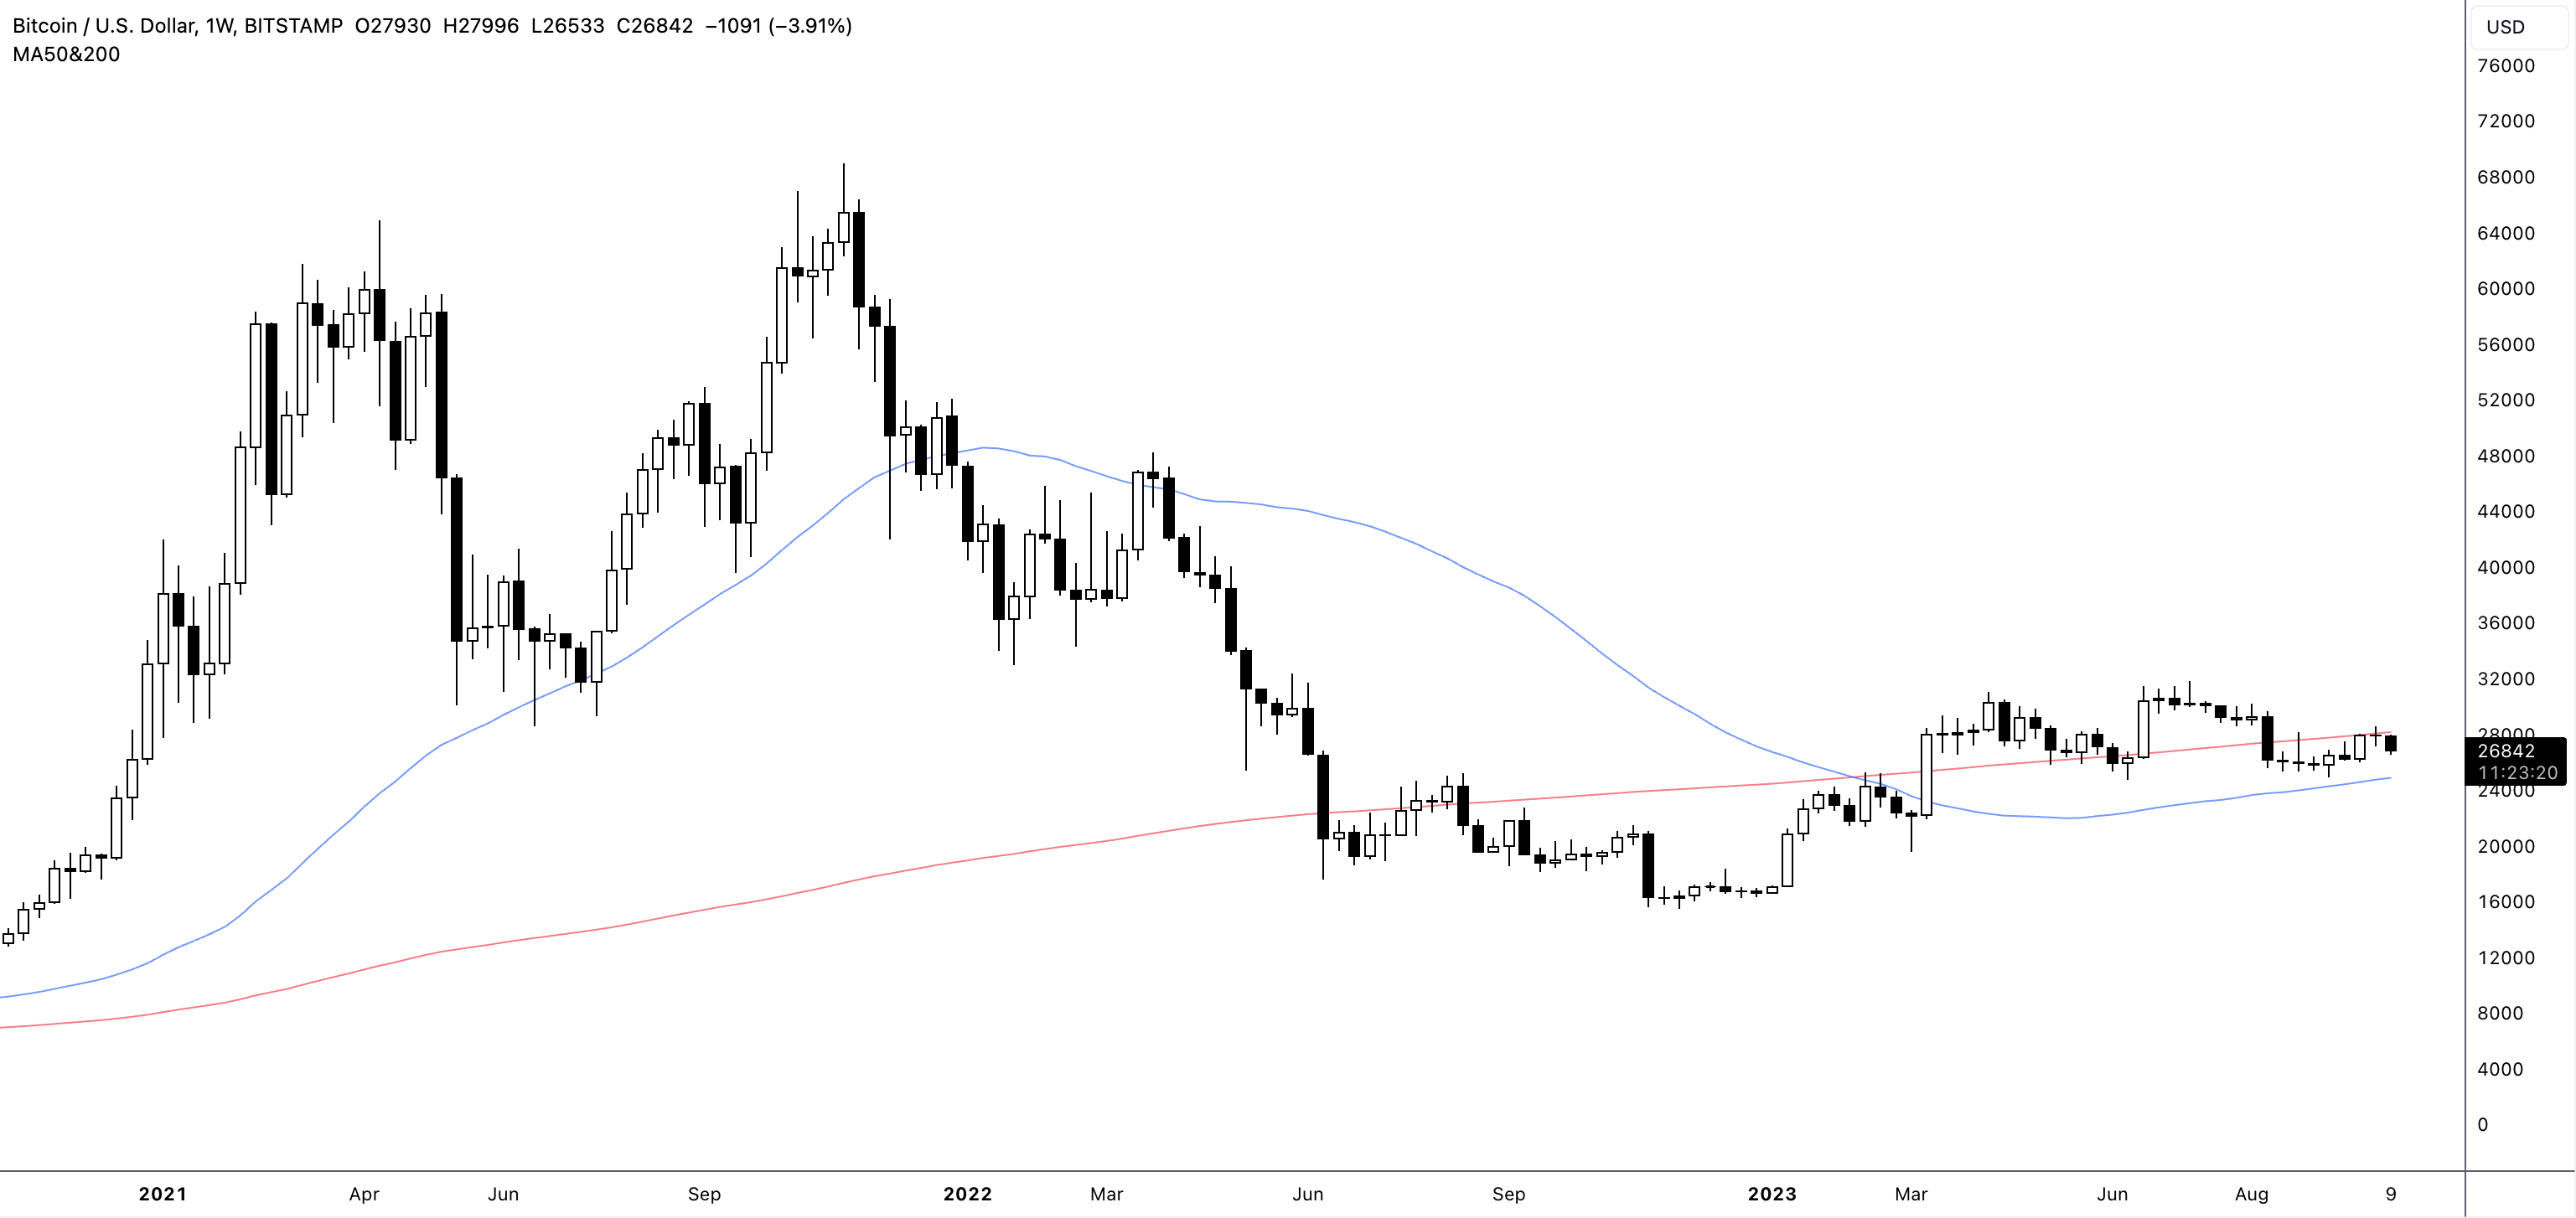
\includegraphics[width=\textwidth]{./assets/img/bitcoin_moving_averages.png}
    \caption{Figure shows the 50-day \gls{ema} in blue and the 200-day \gls{ema} in red applied to \gls{btc} on a weekly \gls{tf} from October 2020 to October 2023.}
    \label{fig:bitcoin_moving_averages}
\end{figure}

% Bollinger Bands
\subsection{Bollinger Bands}
\label{sub:BB}
John Bollinger developed the \gls{bb} in the early 1980's, building on the work of several earlier researchers. These include Wilfrid Ledoux's work on trading bands in 1960, Chester Keltner's introduction of the Keltner channel \citep{keltner1960make}, J.M. Hurst's studies involving graphical representations of price structures, the popularisation of percentage bands in the 1970's (whose specific origin remains unknown), and Richard Donchian's contribution with the Donchian channels \citep{bollinger2023}.
\newline
\newline
\gls{bb} are used to asses the relative highs and lows of an asset's price. They are made up of two bands, each representing a positive and negative \gls{std} from a 20-day \gls{sma}. These bands allow traders to identify potential overbought conditions, indicated by prices continuously touching the upper band, known as $\text{BOLU}$, and oversold conditions, indicated by prices continuously touching the lower band, known as $\text{BOLD}$. See figure \ref{fig:bollinger_bands} for an illustration.

\begin{figure}[ht]
    \centering
    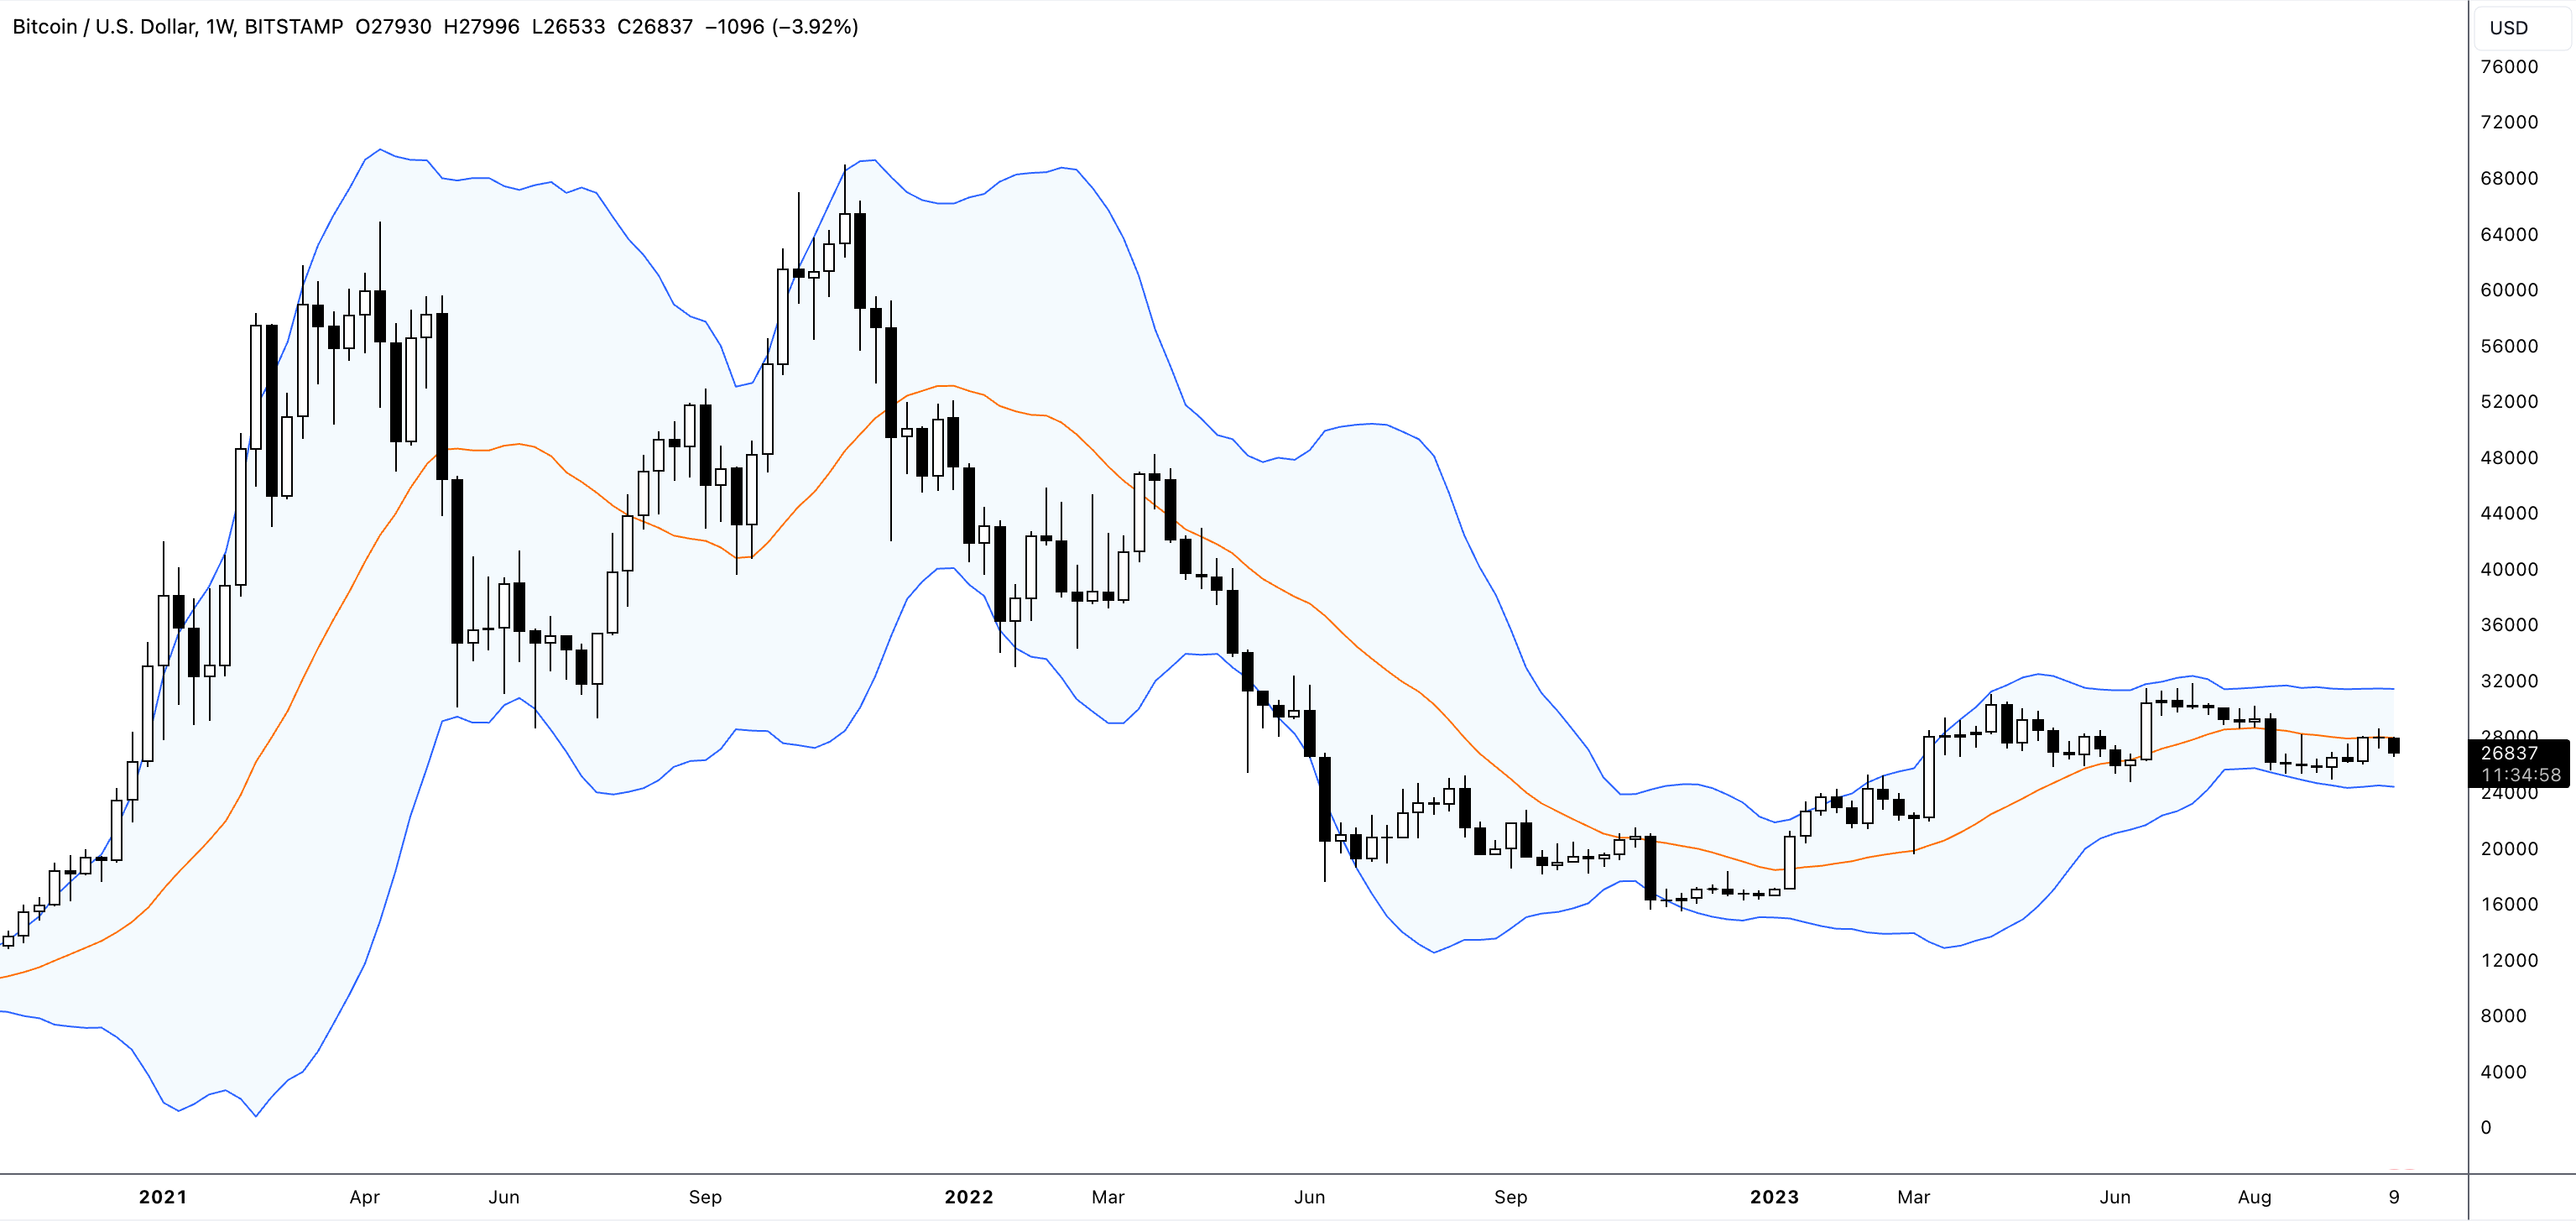
\includegraphics[width=\textwidth]{./assets/img/bitcoin_bollinger_bands.png}
    \caption{Figure shows the \gls{bb} applied to \gls{btc} on a weekly \gls{tf} from October 2020 to October 2023.}
    \label{fig:bollinger_bands}
\end{figure}

\noindent
The upper bands are calculated using the equation \ref{eq:bb_upper_band} and the lower bands using the equation \ref{eq:bb_lower_band}. Where, the \gls{tp} can be calculated by (High + Low + Close) / 3), $n$ is the number of days in the smoothing period, $m$ the number of \glspl{std} and $\sigma [\text{TP}, n]$ the \gls{std} over the last $n$ periods of \gls{tp}.

\myequations{Computing the upper Bollinger Band}
\begin{equation}
    \centering
    \text{BOLU} = \text{MA}(\text{TP}, n) + m \cdot \sigma [\text{TP}, n]
    \label{eq:bb_upper_band}
\end{equation}

\myequations{Computing the lower Bollinger Band}
\begin{equation}
    \centering
    \text{BOLD} = \text{MA}(\text{TP}, n) - m \cdot \sigma [\text{TP}, n] 
    \label{eq:bb_lower_band}
\end{equation}

% Relative Strength Index
\subsection{Relative Strength Index}
\label{sub:RSI}
The \gls{rsi} is a momentum indicator developed by J. Welles Wilder Jr. and first introduced in 1978 in his book \textit{New Concepts in Technical Trading Systems} \citep{Wilder_1978}. Its primary purpose is to measure the speed and magnitude of recent price changes in an asset, providing an indication of whether an asset is currently overbought or oversold on a scale of zero to 100. In the context of the \gls{rsi}, the standard overbought and oversold thresholds are typically set at 70 and 30 respectively, with values above 70 indicating overbought conditions and values below 30 indicating oversold conditions.
\newline
\newline
The \gls{rsi} is calculated using equation \ref{eq:relative_strength_index}. The \gls{rs} is obtained through a three-step calculation process. Firstly, the average daily percentage gains and losses over a predetermined look-back period $n$ of typically 14 days, are computed. Subsequently, the averages of previously calculated gains and losses are multiplied by $n-1$, and the current daily percentage gain or loss is added to emphasize the present price trends. The gain and loss calculations are divided by $n$ to receive their respective arithmetic mean. This computation is commonly referred to as \gls{smma}. Finally, the ratio between the computed \gls{smma} of the gain and loss yields the value of $\text{RS}$.

\myequations{Computing the Relative Strength Index}
\begin{equation}
    \centering
    \text{RSI} = 100 - \frac{100}{1 + \text{RS}}
    \label{eq:relative_strength_index}
\end{equation}

\begin{figure}[ht]
    \centering
    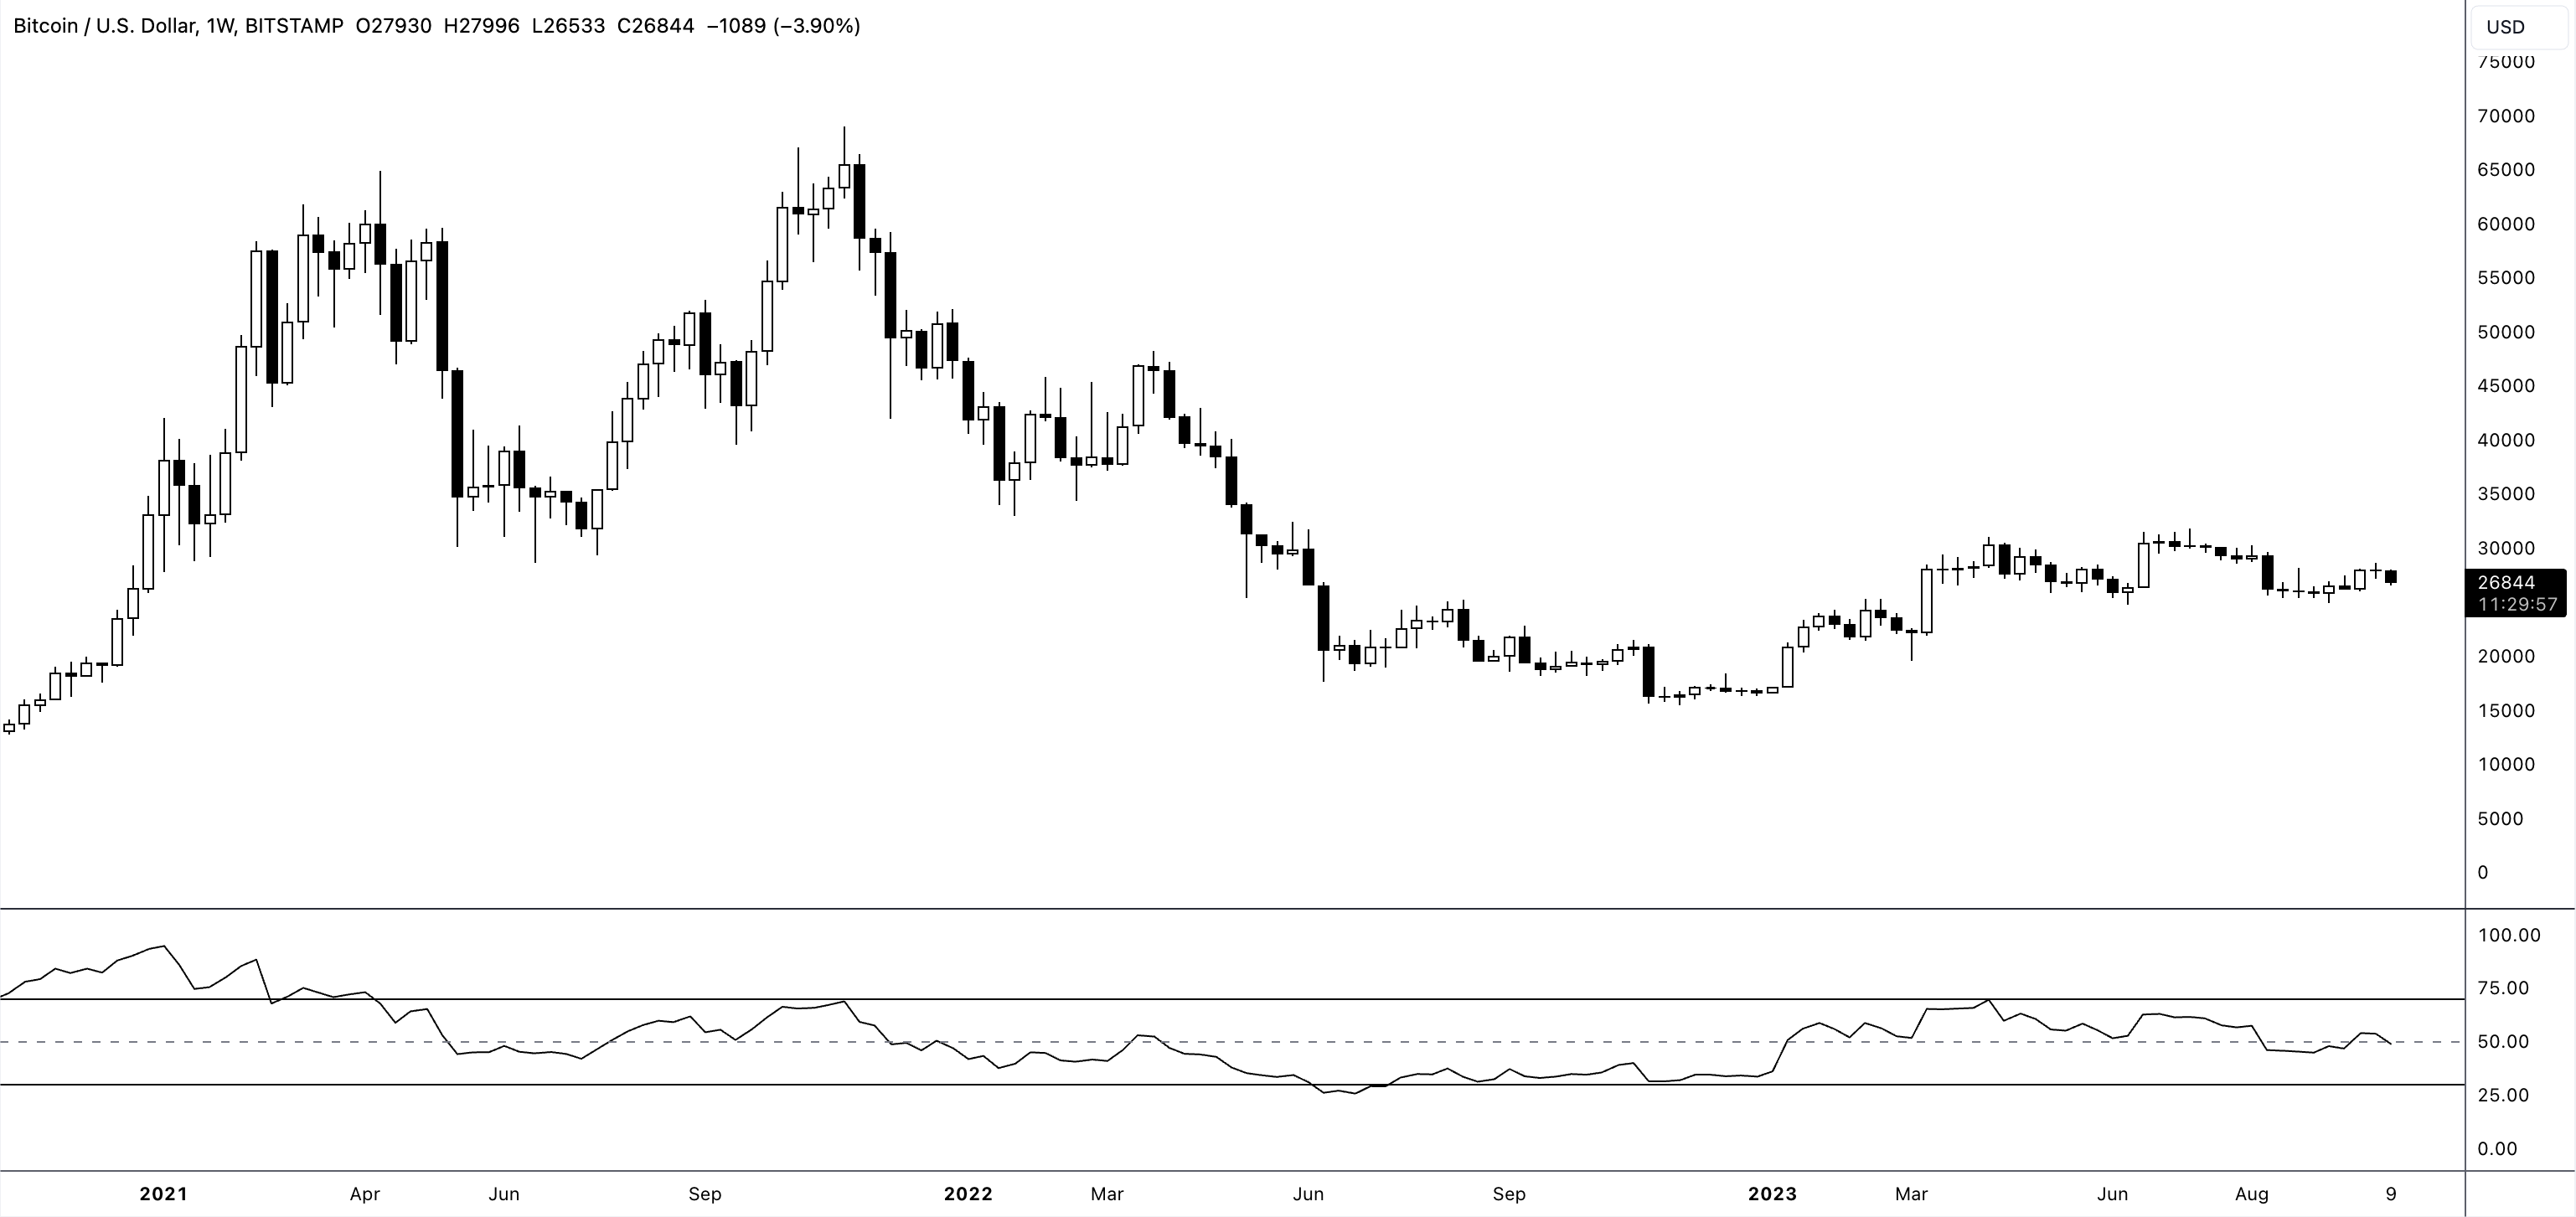
\includegraphics[width=\textwidth]{./assets/img/bitcoin_rsi.png}
    \caption{Figure shows the \gls{rsi} applied to \gls{btc} on a weekly \gls{tf} from October 2020 to October 2023.}
    \label{fig:relative_strength_index}
\end{figure}

% MACD
\subsection{Moving Average Convergence Divergence}
\label{sub:MACD}
Determining the precise origins of the \gls{macd} indicator is difficult, as even its inventor, Gerald Appel, remains vague in his 2005 book \textit{Technical Analysis: Power Tools for Active Investors}. Appel states that the \gls{macd} was developed in the late 1970s, although he does not cite any specific sources \citep{appel2005technical}. However, it is evident that his 1985 report, titled \textit{The Moving Average Convergence-divergence Trading Method: Advanced Version} \citep{appel1985moving} is a refined version of his initial work on the \gls{macd}.
\newline
\newline
The \gls{macd} is a tool used by traders to objectively monitor the correlation between two distinct \glspl{ma}. Fundamentally, the \gls{macd} is comprised of the difference between a faster \gls{ma} (representative of short-term market trends) and a slower \gls{ma} (reflecting longer-term trends). According to the tech report \textit{A Quick Tutorial in MACD: Basic Concepts}, Appel uses two separate sets of \glspl{ma} to calculate \glspl{macd} \citep{appel2008quick}. One set includes a 26-day and 12-day \gls{ema}, while the other set consists of a 39-day and 19-day \gls{ema}. Equation \ref{eq:macd} employs the 26-day and 12-day \gls{ema} in the calculation of the \gls{macd}. Furthermore, the \gls{macd} incorporates a signal line, which typically uses the 9-day \gls{ema} of the \gls{macd} line.

\myequations{Computing the Moving Average Convergence Divergence}
\begin{equation}
    \centering
    \text{MACD} = \text{12-Period} \text{ EMA} - \text{26-Period} \text{ EMA}
    \label{eq:macd}
\end{equation}

\noindent
When the short-term average is higher than the long-term average, the \gls{macd} signals upward momentum. On the other hand, when the short-term average drops below the long-term average, it signals downward momentum as illustrated in figure \ref{fig:macd_momentum}

\begin{figure}[ht]
    \centering
    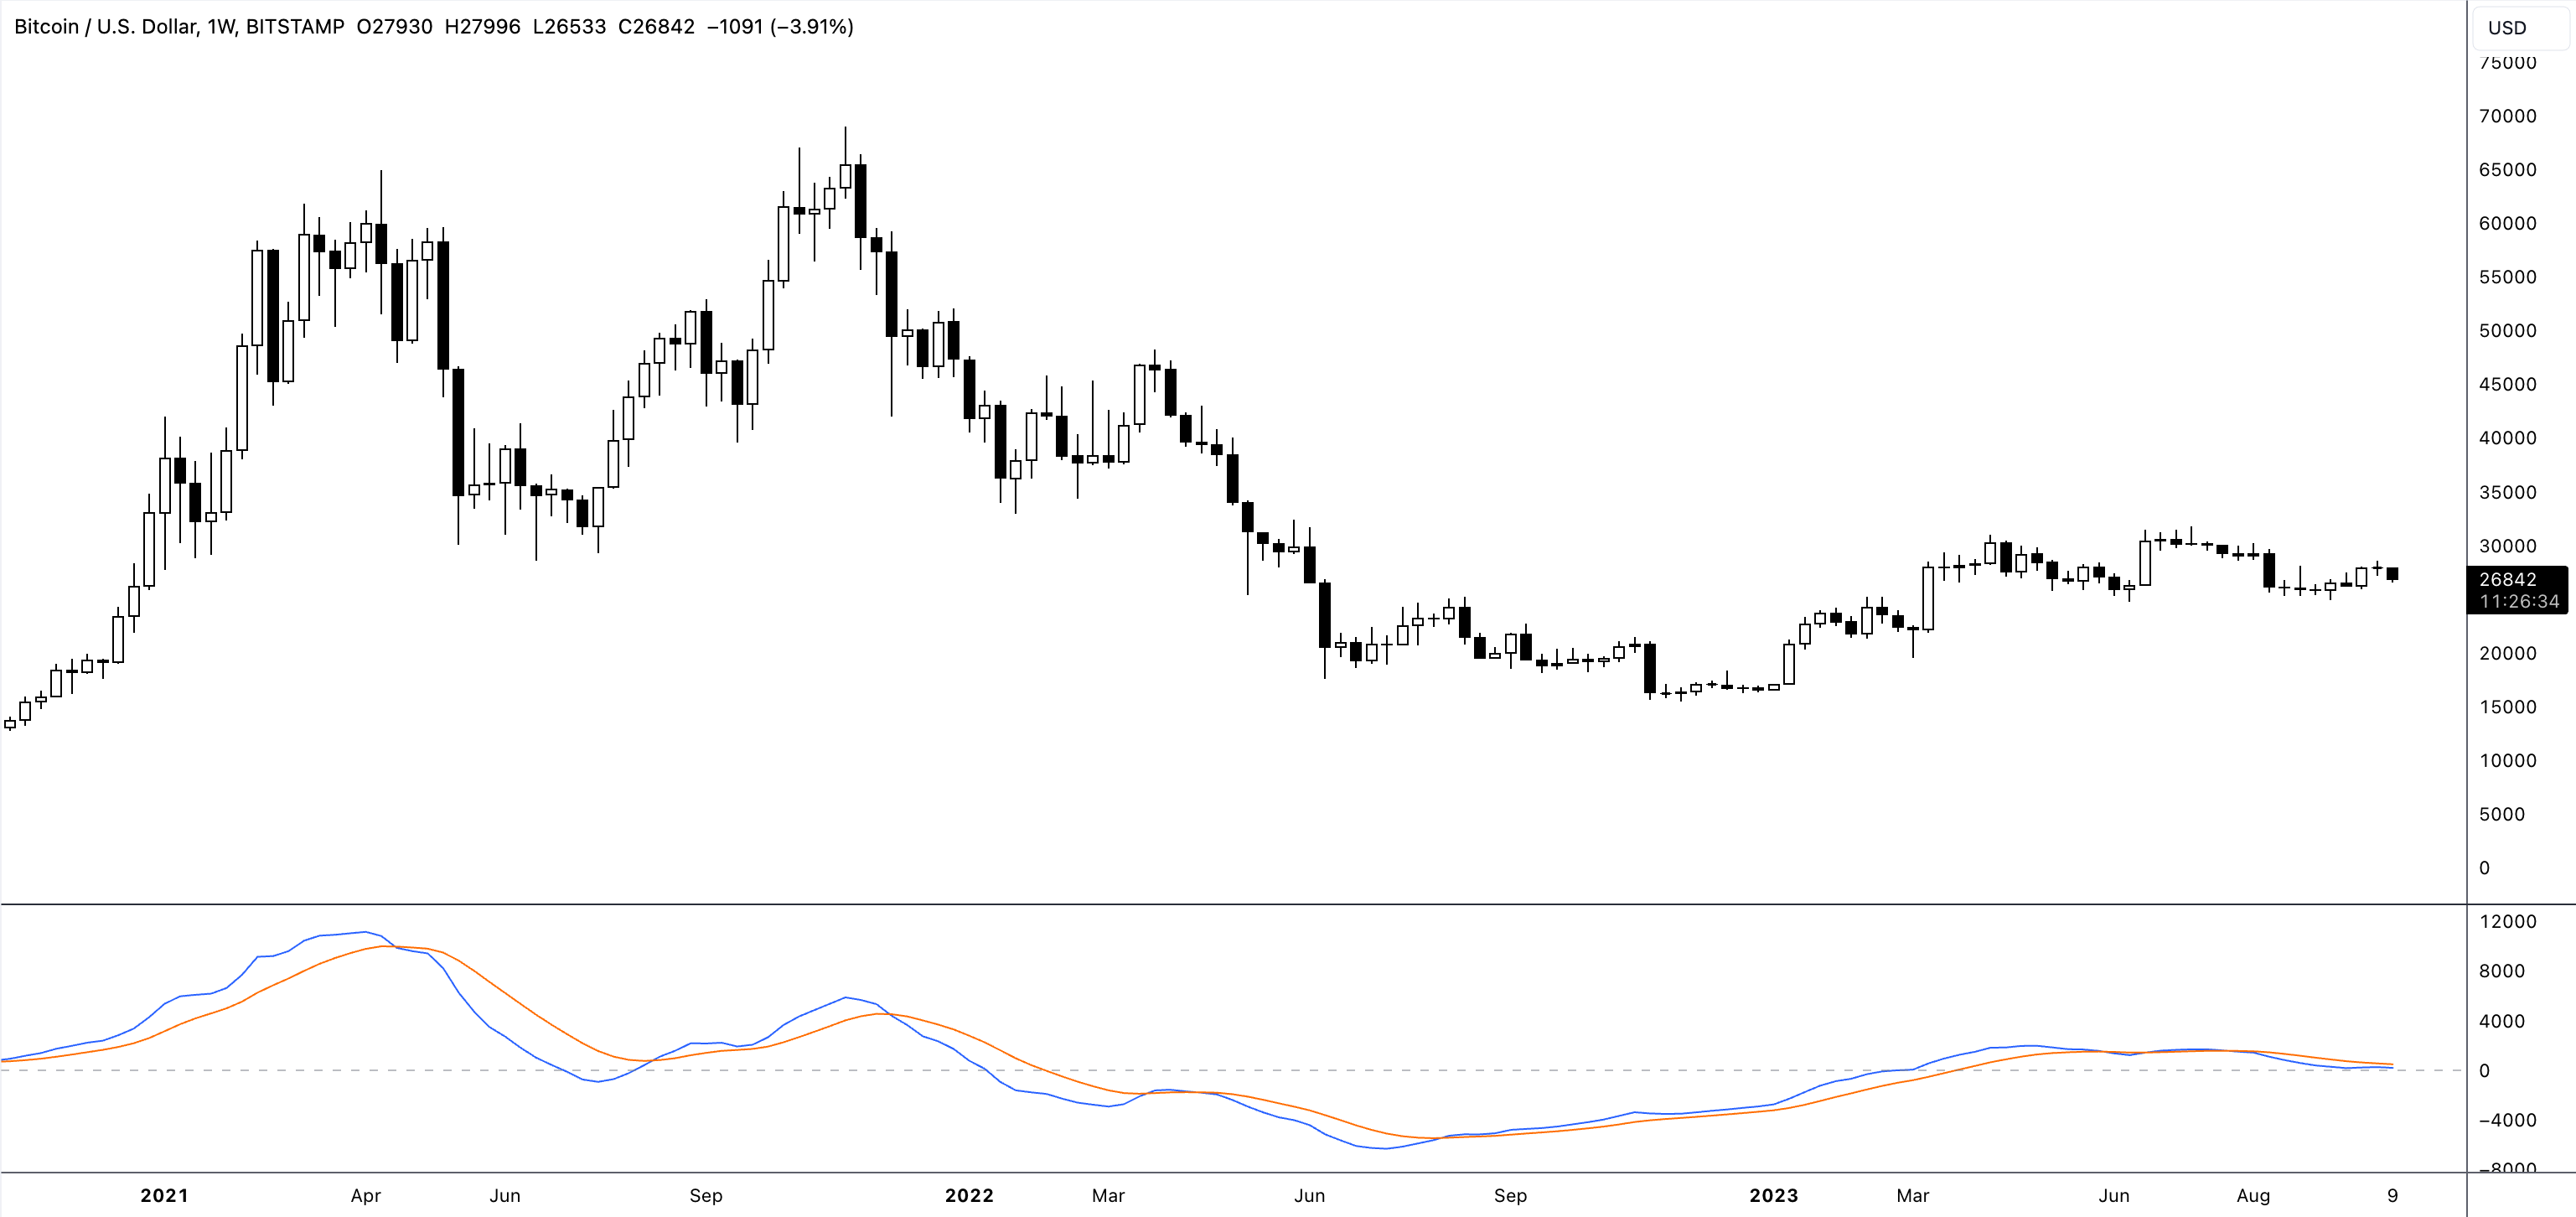
\includegraphics[width=\textwidth]{./assets/img/bitcoin_macd.png}
    \caption{Figure shows the \gls{macd} applied to \gls{btc} on a weekly \gls{tf} from October 2020 to October 2023.}
    \label{fig:macd_momentum}
\end{figure}

% CCI
\subsection{Commodity Channel Index}
\label{sub:CCI}
Originally developed by Donald Lambert and introduced in his book \textit{Commodity Channel Index: Tools for Trading Cyclical Trends} \citep{lambert1983commodity}, the \gls{cci} is an oscillator that has gained considerable popularity since its inception. While initially designed for commodities, it has evolved into a widely used technical indicator for assessing cyclical trends in equities and currencies.
\newline
\newline
Like many oscillators, the primary purpose of the \gls{cci} is to identify overbought (above +100) and oversold (below -100) levels in the market. This is achieved by measuring the deviation of an asset's \gls{tp} (see section \ref{sub:BB}) from its statistical average over a specific period, often using the 20-day \gls{sma}. Equation \ref{eq:cci} outlines the calculation of the \gls{cci}, where $n$ is the number of periods. The formula in the denominator calculates the mean deviation, i.e., the absolute difference between each typical price and the \gls{sma} over $n$ periods.

\myequations{Calculation of the Commodity Channel Index}
\begin{equation}
    \centering
    \text{CCI} = \frac{\text{TP} - \text{ SMA}}{0.015 \cdot \frac{\sum_{i=1}^n | \text{TP}_i - \text{ SMA} |}{n}}
    \label{eq:cci}
\end{equation}

\begin{figure}[ht]
    \centering
    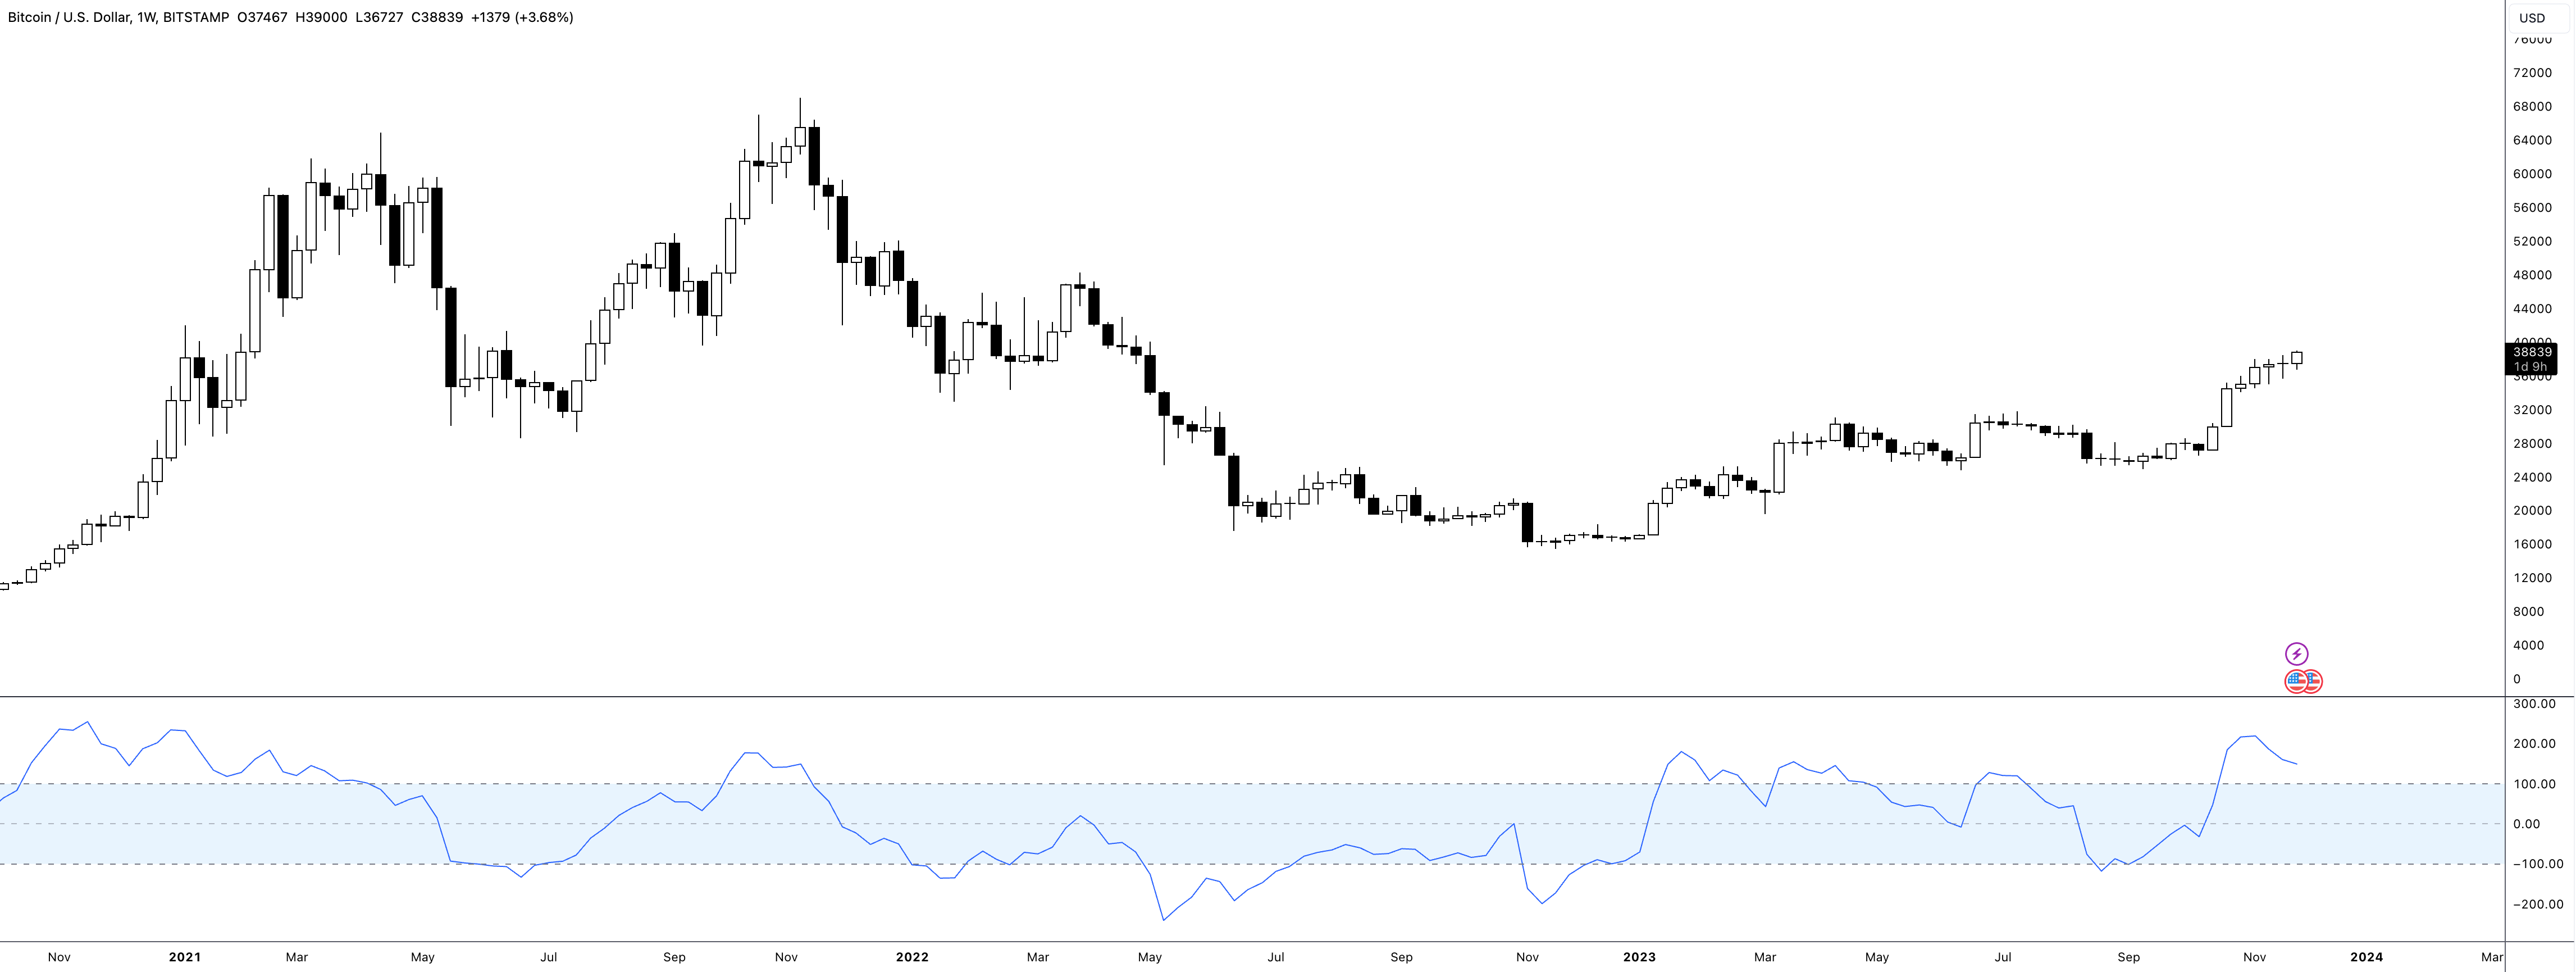
\includegraphics[width=\textwidth]{./assets/img/btc-cci.png}
    \caption{Figure shows the \gls{cci} applied to \gls{btc} on a weekly \gls{tf} from October 2020 to December 2023.}
    \label{fig:cci}
\end{figure}

% OBV
\subsection{On-Balance Volume}
\label{sub:OBV}
Joseph Granville introduced \gls{obv} in 1963 in his book \textit{Granville's New Key to Stock Market Profits} \citep{granville1963new}. As a momentum indicator, \gls{obv} uses volume flow to anticipate changes in the price of an asset.
\newline
\newline
Granville's concept was based on the belief that volume plays a central role in market dynamics. The \gls{obv} was designed to predict major market movements by examining shifts in volume. Grandville argued that a significant increase in volume, unaccompanied by a significant change in price, would eventually lead to an upward or downward price movement.
\newline
\newline
The calculation of $\text{OBV}_t$ is determined by equation \ref{eq:obv}. It involves adding $\text{OBV}_{t-1}$ and either the current volume, zero, or the negative of the current volume, depending on the relationship between the closing price at time $t$ and $t-1$.

\myequations{Calculation of the On-Balance Volume}
\begin{equation}
    \centering
    \text{OBV}_t = \text{OBV}_{t-1} + \left\{ \begin{array}{rcl}
    \text{volume,} \quad \text{if close}_t > \text{close}_{t-1} \\
    0, \quad \text{if close}_t = \text{close}_{t-1} \\
    \text{-volume,} \quad \text{if close}_t < \text{close}_{t-1}
    \end{array}\right.
    \label{eq:obv}
\end{equation}

\noindent
The theory behind \gls{obv} revolves around the distinction between smart money (institutional investors) and less sophisticated retail investors. When institutional investors buy an asset that retail investors are selling, volume can increase even if the price remains relatively stable. Eventually, the increased volume drives the price up. As larger investors begin to sell, smaller investors begin to buy.
\newline
\newline
Analysts use \gls{obv} volume figures to track large institutional investors, often referred to as smart money, treating divergences between volume and price as indicators of the relationship between smart money and the broader market. Such divergences can signal opportunities to trade against prevailing trends, highlighting instances where smart money is driving up prices before strategically selling.

\begin{figure}[ht]
    \centering
    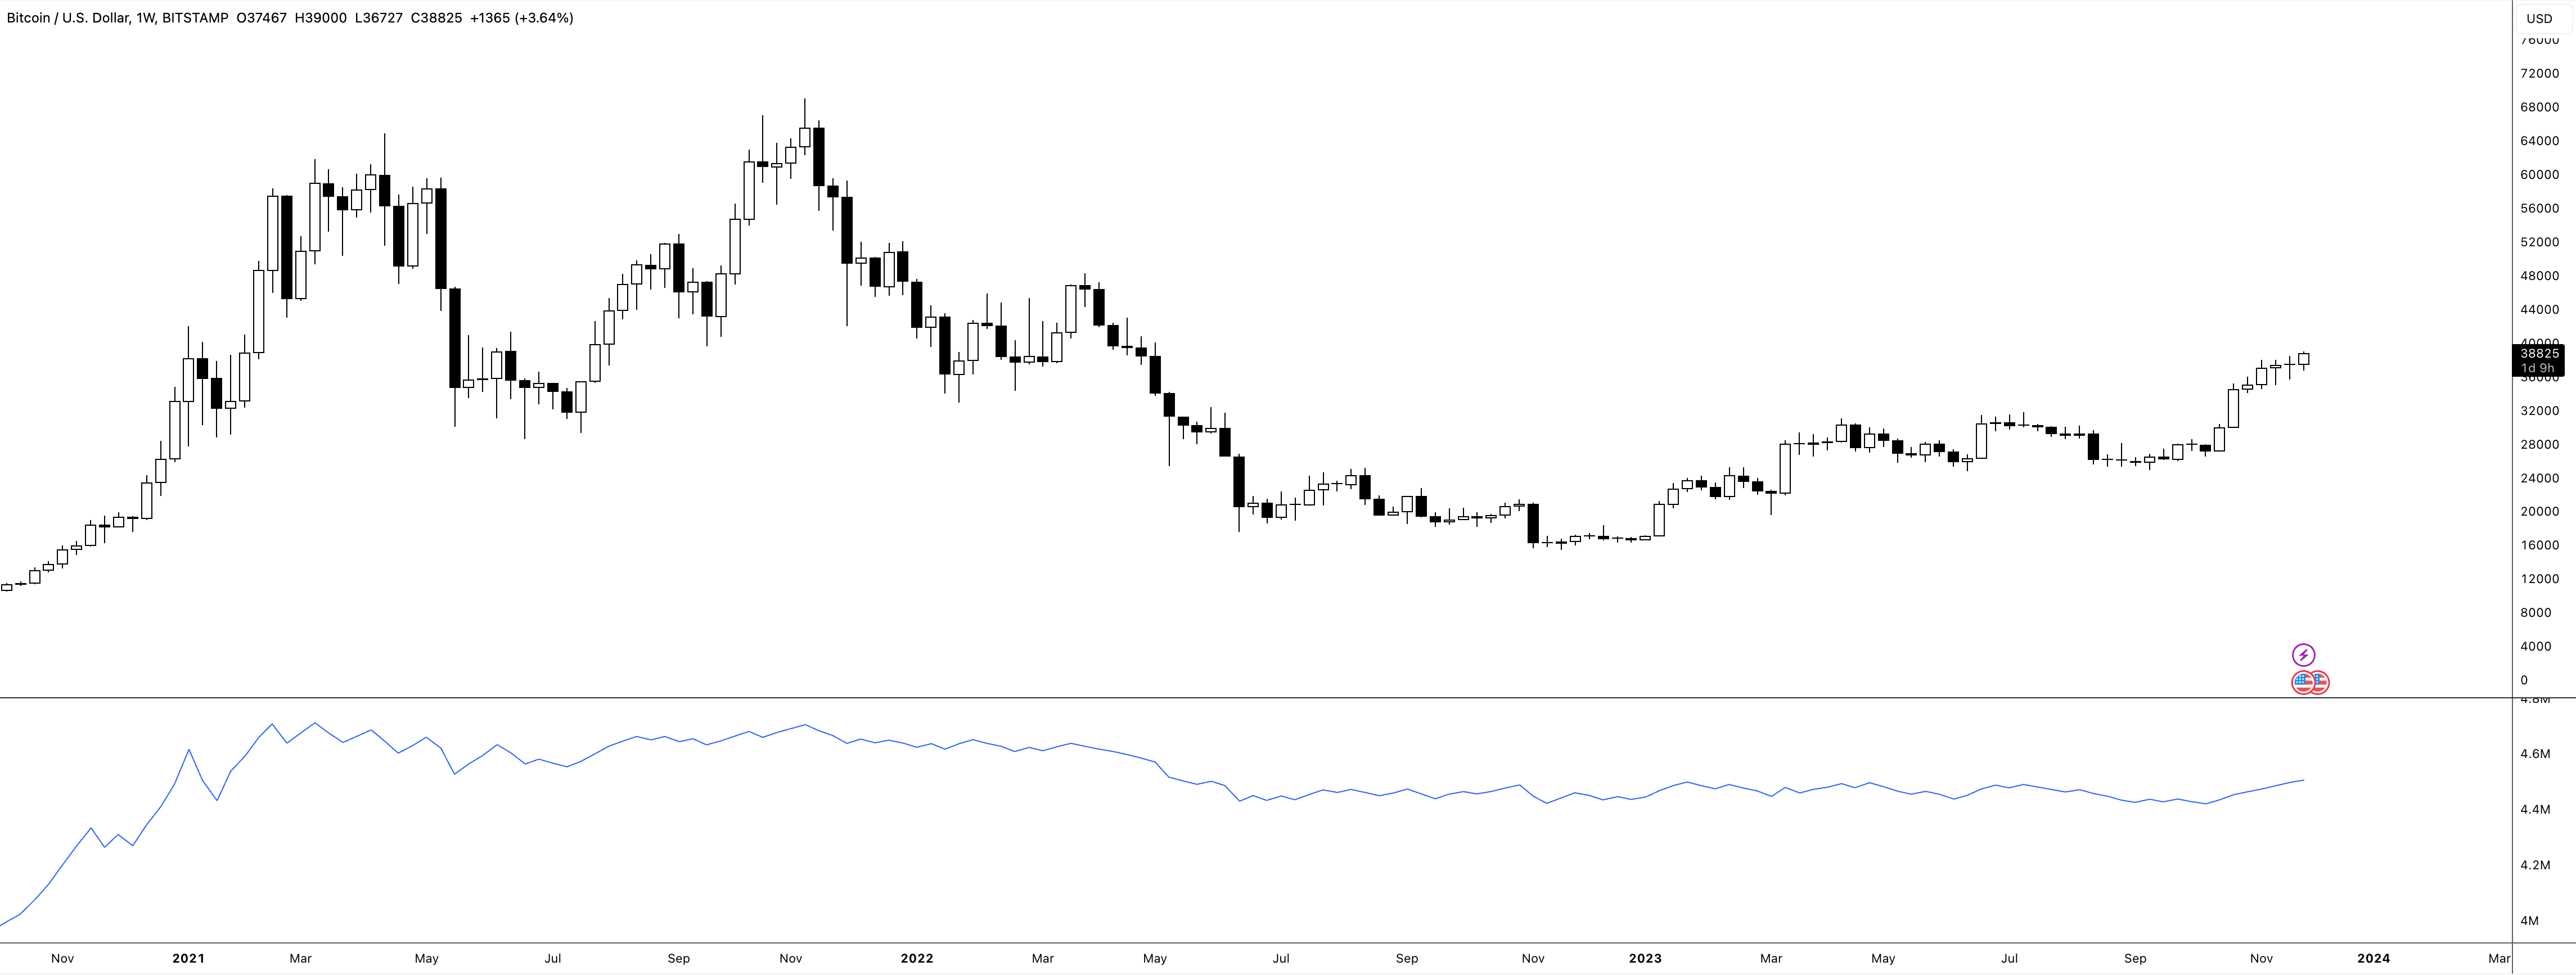
\includegraphics[width=\textwidth]{./assets/img/btc-obv.png}
    \caption{Figure shows the \gls{obv} applied to \gls{btc} on a weekly \gls{tf} from October 2020 to December 2023.}
    \label{fig:obv}
\end{figure}

% AD
\subsection{Accumulation/Distribution Indicator}
\label{sub:AD}

% Introduction
Market analyst Marc Chaikin developed the \gls{ad} to measure the cumulative flow of money into or out of an asset. This indicator provides valuable insight into the complex relationship between price and volume dynamics \citep{Yu_2023}.
\newline
\newline
% Equation
The calculation of the \gls{ad} involves three steps. First, the \gls{mfm} is calculated using the equation \ref{eq:MFM}, where $\text{close}$ is the closing price and $\text{low}$ and $\text{high}$ are the corresponding lowest and highest prices achieved during the period. Secondly, the \gls{mfv} is calculated by multiplying the \gls{mfm} by the current volume. Finally, the current \gls{ad} is calculated by multiplying the previous \gls{ad} by the \gls{mfv}.

\myequations{Calculation of the Money Flow Multiplier}
\begin{equation}
    \centering
    \text{MFM} = \frac{\text{(Close - Low) - (High - Close)}}{\text{High - Low}}
    \label{eq:MFM}
\end{equation}

\noindent
% Interpretation
A rising \gls{ad} line indicates accumulation (buying pressure), while falling \gls{ad} indicates distribution (selling pressure). Traders use these trends to anticipate potential price movements and assess the strength of ongoing trends based on volume and the direction of the trend.

\begin{description}
    \item[Uptrends:] A rising \gls{ad} line confirms strong support for the uptrend and indicates sufficient money flow.
    \item[Downtrends:] A falling \gls{ad} line in downtrends indicates support for the downtrend, reflecting money flowing out of the asset.
    \item[Uptrend divergence:] When the \gls{ad} line falls during an uptrend, it indicates a divergence. This may indicate that the rise in the assets price lacks strong support from accumulation volume and may signal a reversal.
    \item[Downtrend divergence:] In a downtrend with a rising \gls{ad} line, distribution volume may be decreasing, possibly signalling a reversal.
\end{description}

\begin{figure}[ht]
    \centering
    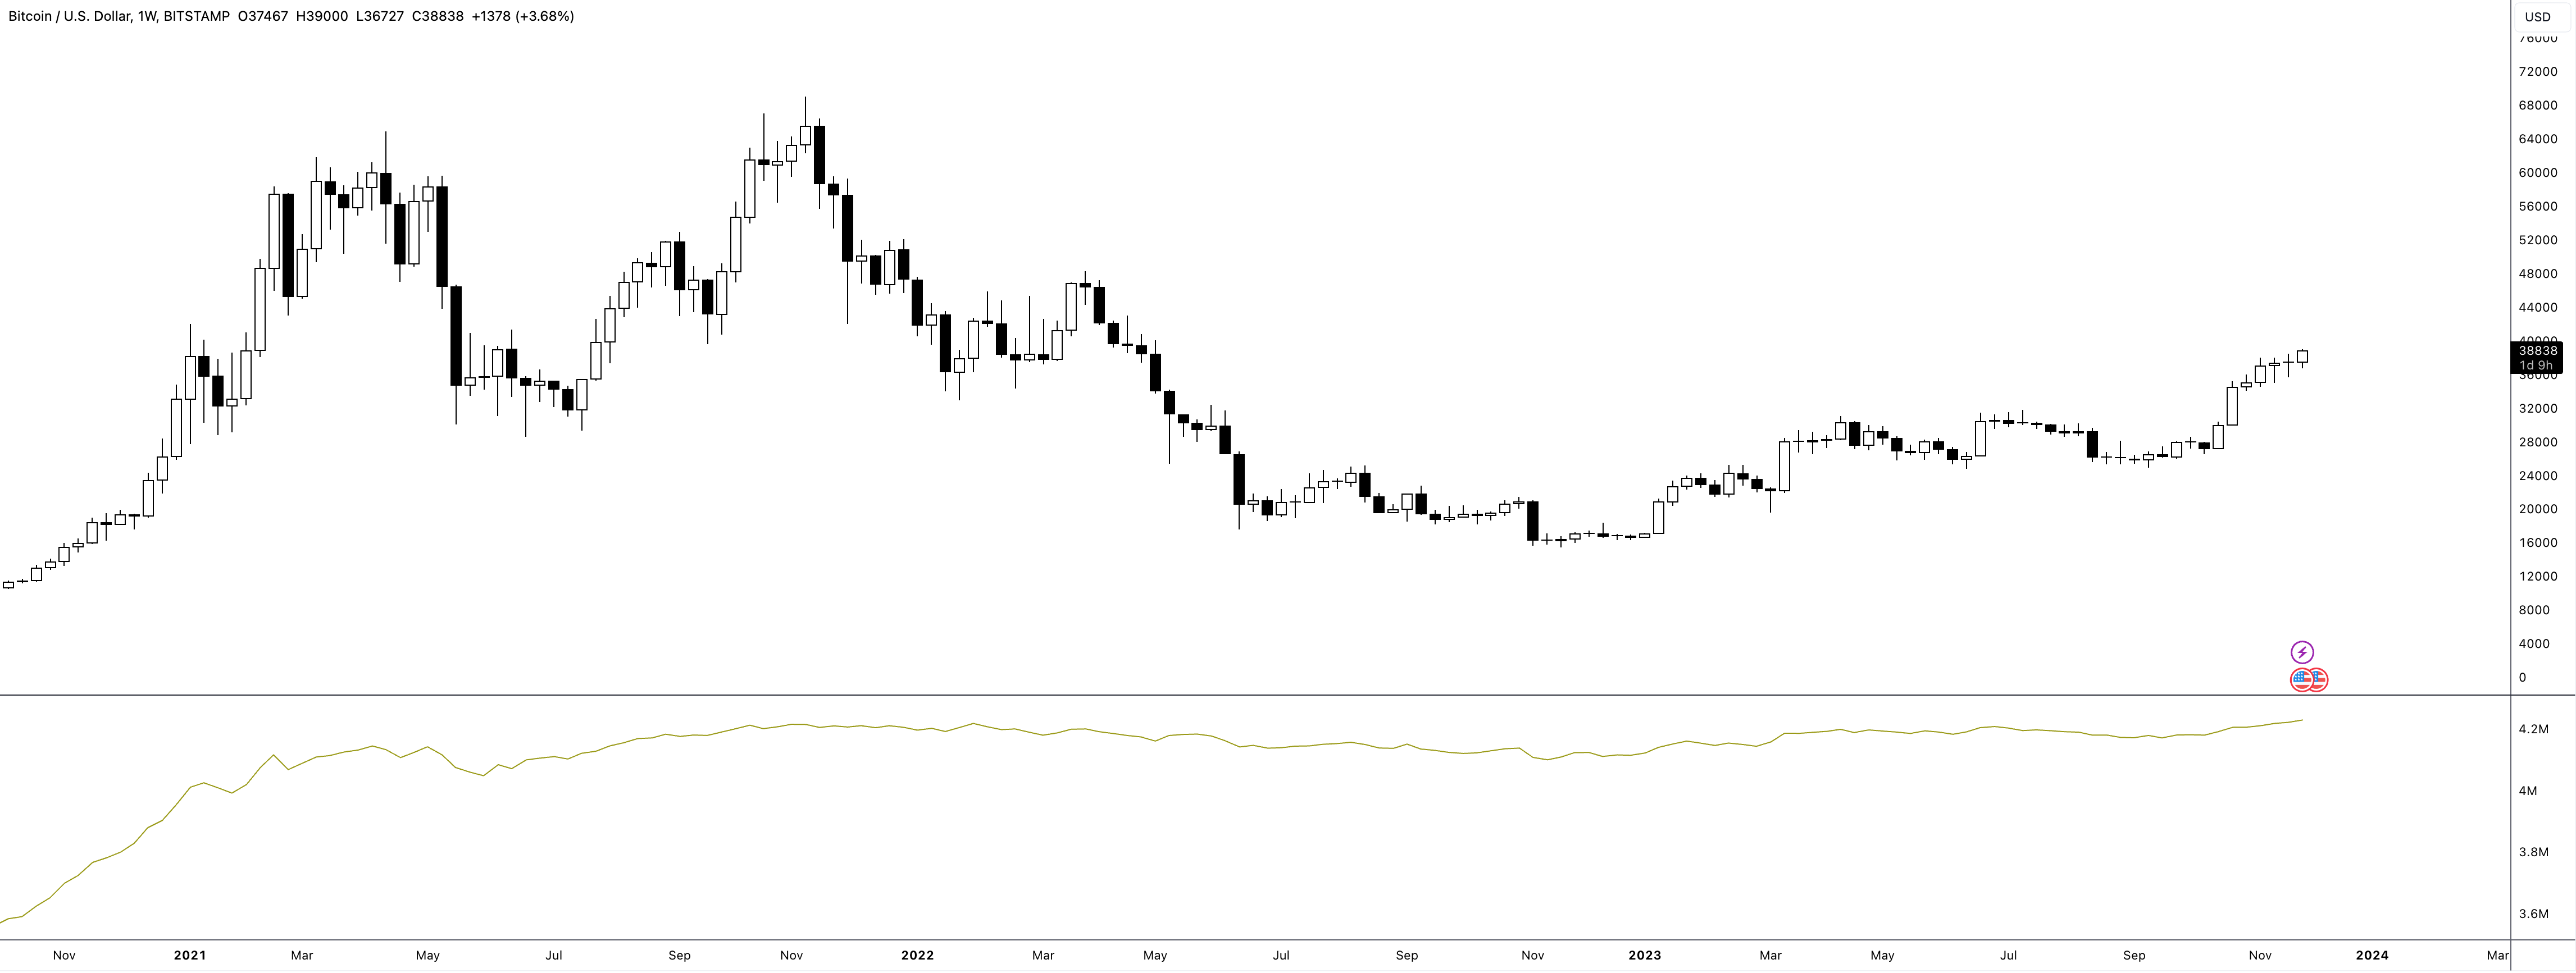
\includegraphics[width=\textwidth]{./assets/img/btc-ad.png}
    \caption{Figure shows the \gls{ad} applied to \gls{btc} on a weekly \gls{tf} from October 2020 to December 2023.}
    \label{fig:ad}
\end{figure}

% ADX
\subsection{Average Directional Index}
\label{sub:ADX}
In addition to the \gls{rsi}, J. Welles Wilder Jr. introduced the \gls{adx} in his book \textit{New Concepts in Technical Trading Systems} \citep{Wilder_1978} in 1978. Unlike the \gls{rsi}, the \gls{adx} is a lagging indicator and is derived from two other indicators developed by J. Welles Wilder Jr. namely the \gls{+di} and the \gls{-di}. The \gls{adx} combines these indicators and smooths the result with a \gls{ma}.
\newline
\newline
To calculate the \gls{+di}, a smoothing period is defined (usually set at 14 days, as suggested by J. Welles Wilder Jr. in his book). The \gls{+di} is obtained by subtracting the previous high from the current high for the period, dividing the result by the true range for the period, and multiplying it by 100. The true range is defined as the largest of the following: the current high minus the current low, the current high minus the previous close, or the absolute value of the current low minus the previous close.
\newline
\newline
Similarly, the \gls{-di} is calculated by selecting a smoothing period, subtracting the current low from the previous low for the period, dividing it by the true range for the given period, and multiplying the result by 100. The \gls{dmi} is then calculated by subtracting \gls{-di} from \gls{+di}, dividing the absolute value of this result by the absolute sum of \gls{+di} and \gls{-di}, and multiplying by 100.
\newline
\newline
To obtain the first \gls{adx}, the \gls{dmi} is calculated for 14 periods. The equation \ref{eq:Average_Directional_Index} then calculates the subsequent \glspl{adx}.

\myequations{Average Directional Index}
\begin{equation}
    \centering
    \text{\gls{adx}} = \frac{(\text{Prior ADX} \cdot 13) + \text{Current ADX}}{14}
    \label{eq:Average_Directional_Index}
\end{equation}

\begin{figure}[ht]
    \centering
    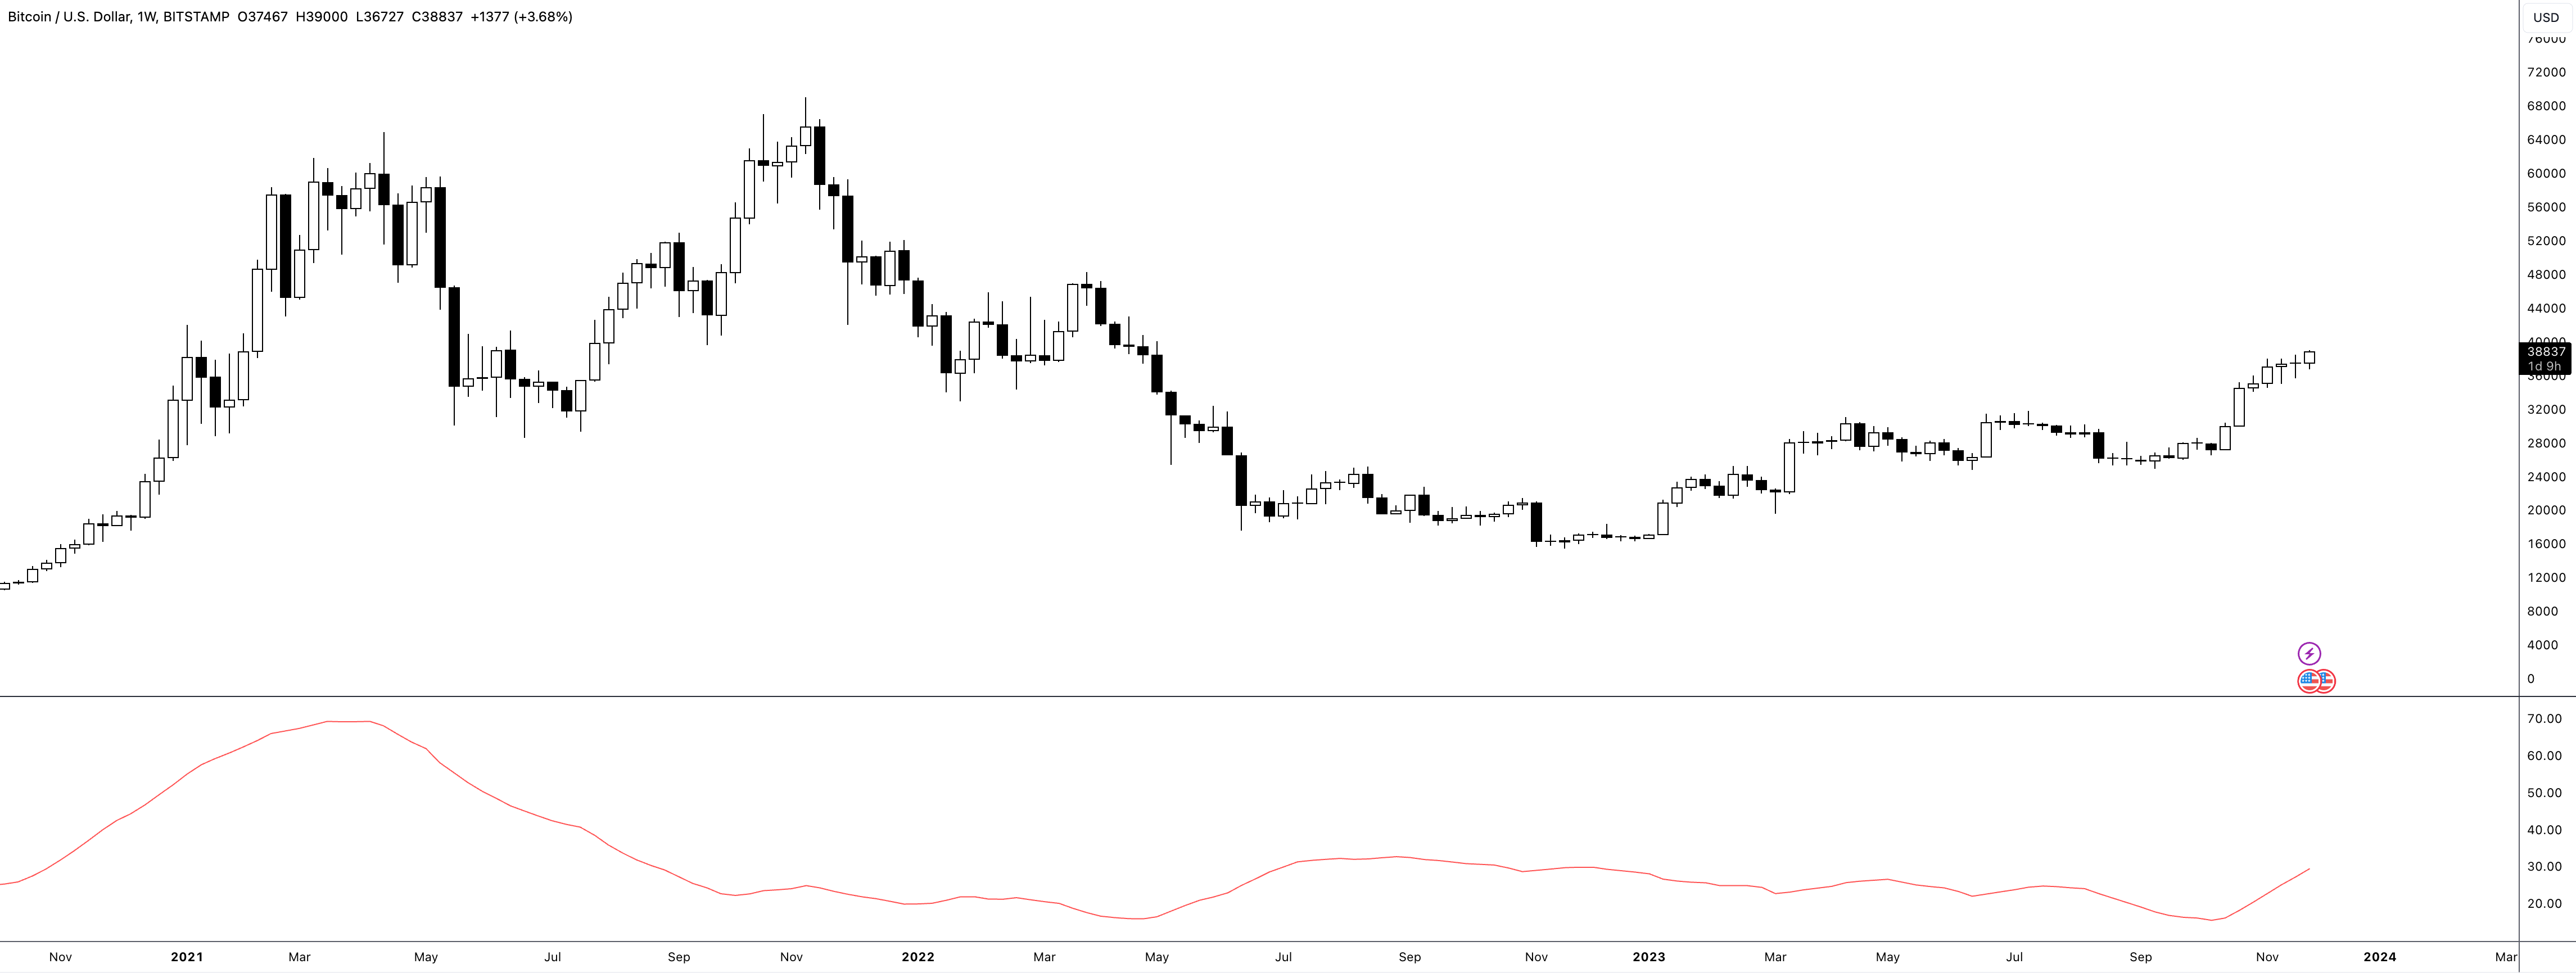
\includegraphics[width=\textwidth]{./assets/img/btc-adx.png}
    \caption{Figure shows the \gls{adx} applied to \gls{btc} on a weekly \gls{tf} from October 2020 to December 2023.}
    \label{fig:adx}
\end{figure}

\noindent
The \gls{adx} is a valuable tool for investors to assess the strength of a trend, while the \gls{+di} and \gls{-di} help to determine the direction of a trend.
\newline
\newline
The \gls{adx} is useful in determining the strength of a trend. A reading above 25 indicates a strong trend, while a reading below 20 indicates a weaker trend. Trading signals can be generated by crossing the \gls{-di} and \gls{+di} lines. For example, if the \gls{+di} crosses the \gls{-di} and the \gls{adx} is above 20, this signals a potential buying opportunity. Conversely, if the \gls{-di} crosses the \gls{+di} and the \gls{adx} is above 20, this is an opportunity to go short.
\newline
\newline
These crosses also guide exit strategies for existing trades. For example, in a long position, consider exiting when the \gls{-di} crosses above the \gls{+di}. In addition, a \gls{adx} reading below 20 indicates a trendless market, suggesting caution in entering new trades during such periods.

% TA-Lib
\subsection{TA-Lib}
\label{sub:TA-Lib}
TA-Lib is a widely used Python package for technical analysis of financial market data. It offers over 200 technical indicators and also candlestick-pattern recognition, which will not be used in this thesis. Installing TA-Lib on any device is straightforward and requires the us of HomeBrew and PIP for installation.\footnote{https://ta-lib.github.io/ta-lib-python/install.html, accessed on 06.10.2023}

\begin{verbatim}
    brew install ta-lib
\end{verbatim}

\begin{verbatim}
    pip install TA-Lib
\end{verbatim}

\newpage
\section{Algorithmic Trading}
\label{sec:AlgorithmicTrading}
There is no single, universally accepted definition of algorithmic trading. At its most basic level, it refers to the trading of financial instruments based on some formal algorithm \citep{hilpisch2020python}. An algorithm is a sequence of instructions that a computer must perform to solve a well-defined problem.

\subsection{Alpha}
\label{sub:Alpha}
In the broader landscape of algorithmic trading, there are different motives and objectives. However, this thesis focuses specifically on the singular objective of finding alpha. The use of the term alpha in finance dates back to 1968, when Michael Jensen introduced Jensen's alpha in his paper \textit{The Performance of Mutual Funds in the Period 1945 - 1964} \citep{jensen1968performance}. Initially designed to assess the risk-adjusted returns of a portfolio and its relative performance against the expected market outcomes, Jensen's alpha evolved over time into a broader measure of investment performance, commonly referred to simply as alpha. This term is widely used to characterise returns that exceed those of the overall market or a benchmark index \citep{tulchinsky2019finding}.

\subsection{Trading Strategies}
\label{sub:Trading_Strategies}
Throughout this thesis four different algorithmic trading strategies are used. This strategies are called \gls{sma}-based, momentum, mean reversion and machine learning.

\subsubsection{\gls{sma}-based Trading Strategy}
\label{subsub:SMA}
The first type of algorithmic trading strategy relies on two \glspl{sma}, a faster and a slower one, to generate trading signals and market positioning. The basic idea is that if the shorter-term \gls{sma} crosses the longer-term \gls{sma} in absolute values signals a long market position and the opposite scenario signals a neutral or short market position.

\subsubsection{Momentum Trading Strategy}
\label{subsub:Momentum}
Originating from a paper by \cite{jegadeesh1993returns}, the core idea behind momentum strategies is that financial asset that are trending one direction, will continue to do so for an extended period of time. Thus, an asset that strongly trends upwards signals a long market position and one that strongly trends downward signals a short market position.

\subsubsection{Mean Reversion Trading Strategy}
\label{subsub:Mean_Reversion}
Mean reversion trading strategies assume that the price of an financial asset returns to some trend level if it is currently far enough from it \citep{balvers2000mean}. The distance to its mean can either be negative or positive, with negative implying a long market position and a positive a short market position.

\subsubsection{Machine Learning Trading Strategy}
\label{subsub:ML_Strategy}
Whereas the three previous trading strategies originally stem from the domain of technical analysis (see \ref{sec:TechnicalAnalysis}), this trading strategy utilises predictions of machine and deep learning models to generate long or short market positions. This thesis aims to compare the before mentioned algorithmic trading strategies with two machine learning approaches.

\newpage
\section{Machine Learning}
\label{sec:MachineLearning}
This section provides an introduction to the most essential concept of this thesis, machine learning algorithms.

\subsection{Decision Trees}
\label{sub:DT}

% Introduction & Building Blocks
A \gls{dt} is a non-parametric supervised learning algorithm used for both classification and regression tasks. It has a hierarchical, tree-like structure consisting of a root node, branches, internal nodes and leaf nodes, as shown in figure \ref{fig:decision_tree}.

\begin{figure}[ht]
    \centering
    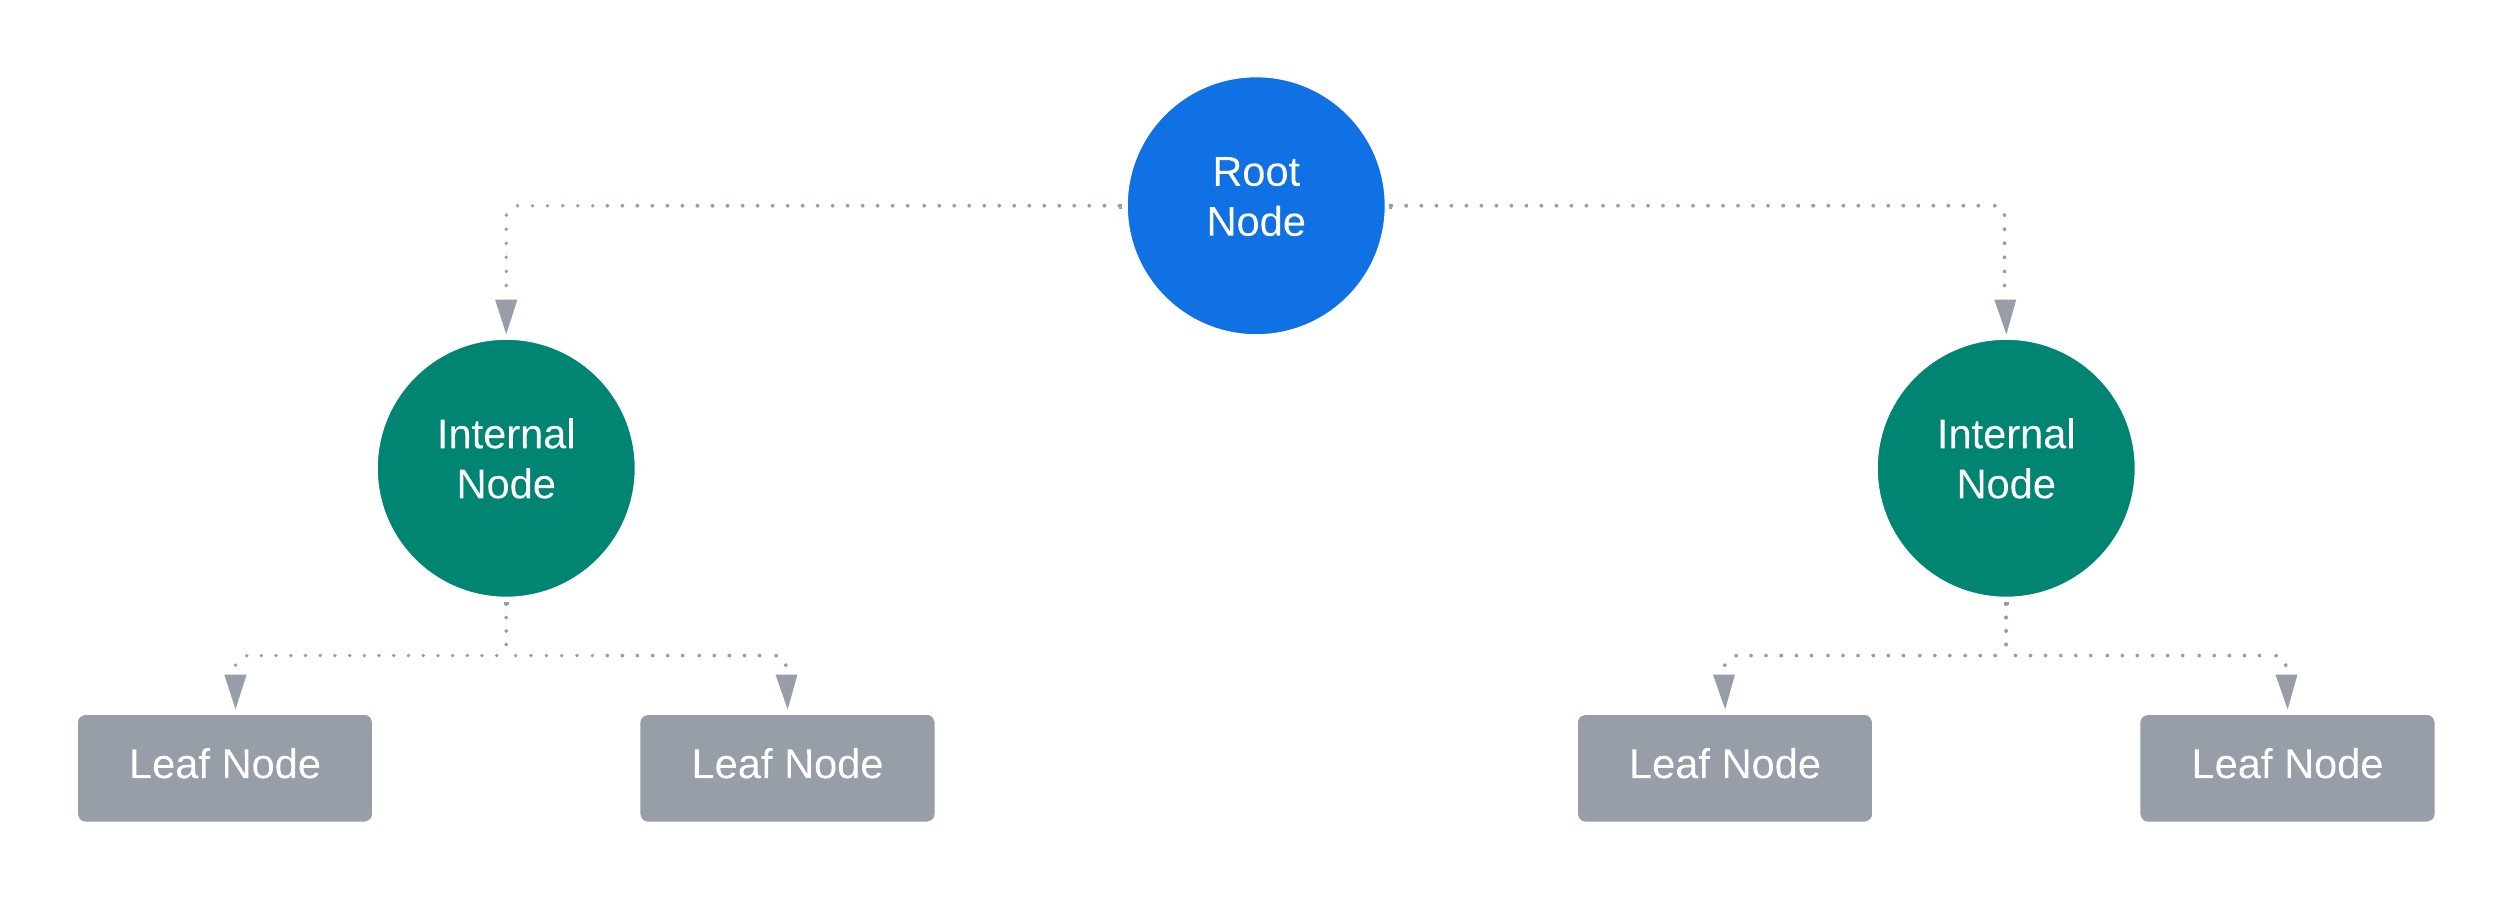
\includegraphics[width=0.75\textwidth]{./assets/img/decision_tree.png}
    \caption{At the top is the root node with no incoming branches. Branches then extend from the root node to reach internal nodes. Further branches then extend from the internal nodes to the leaf nodes. These leaf nodes contain all the possible outcomes within the dataset.}
    \label{fig:decision_tree}
\end{figure}

\noindent
% Learning Process
In the learning process, \glspl{dt} use a divide-and-conquer strategy. They perform a greedy search to find optimal splitting points within the tree. This splitting process occurs in a top-down, recursive manner until all or most of the data points have been assigned a specific class label. Whether all data points are classified into homogeneous sets depends on the complexity of the tree. Smaller trees tend to reach pure leaf nodes, where data points belong to a single class, as illustrated in figure \ref{fig:pure_leaf_node}. However, as trees grow larger, it becomes difficult to maintain purity, often resulting in data fragmentation. This fragmentation, known as overfitting, occurs when too little data falls within a subtree.

\begin{figure}[ht]
    \centering
    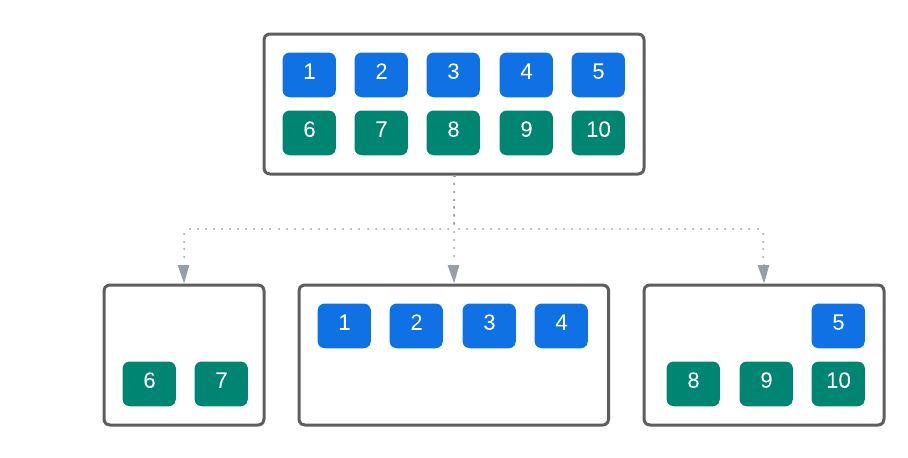
\includegraphics[width=0.75\textwidth]{./assets/img/pure_leaf_node.png}
    \caption{Illustration of a \gls{dt} with two pure leaf nodes on the left and in the middle.}
    \label{fig:pure_leaf_node}
\end{figure}

\noindent
% CART Algorithm
A commonly used algorithm for building \glspl{dt} is the \gls{cart} algorithm introduced by \cite{breiman1984classification}. The \gls{cart} algorithm is widely used to construct decision trees for both classification and regression tasks.
\newline
\newline
\gls{cart} constructs \glspl{dt} through a recursive binary partitioning process. Given a data set $D$ with features $x$ and a target variable $y$, the algorithm aims to partition the data set into subsets $D_1$ and $D_2$ based on a selected feature $x_i$ and a threshold $\theta$ such that

\begin{align*}
    D_1 &= \{ (x, y) \in D \,|\, x_i \leq \theta \} \\
    D_2 &= \{ (x, y) \in D \,|\, x_i > \theta \}
\end{align*}

\noindent
The goal is to identify optimal splits that maximise the purity of the resulting subsets. For classification tasks, purity is often measured by metrics such as Gini impurity, and for regression tasks it may include metrics such as \gls{mse}. The algorithm applies this splitting process recursively to subsets until a stopping criterion is met, such as reaching a predefined depth or having too few data points in a node.
\newline
\newline
% Pruning to reduce complexity
To reduce overfitting and produce more interpretable models, \glspl{dt} favour smaller trees. Complexity reduction is usually achieved through a process called pruning. Pruning selectively removes branches that split on less important features, resulting in simpler and more generalised trees.
\newline
\newline
% Ensembling Methods
To mitigate the problem of overfitting and improve prediction accuracy, \glspl{dt} can be combined using ensemble methods rather than relying on individual trees alone. Ensemble methods combine the outputs of multiple \glspl{dt}, called weak learners. Two prominent ensemble methods are bagging and boosting.

% Bagging (bootstrap aggregation)
\subsubsection{Bagging}
\label{subsub:bagging}
In bagging, a large number of individual weak learners independently make predictions for the target variable. The ensemble then consolidates these predictions through a consensus mechanism. For classification tasks, this is often a majority vote, where the most frequently predicted class among the trees is selected. For regression tasks, a weighted average of the predictions is computed.

% Boosting
\subsubsection{Boosting}
\label{subsub:boosting}
Boosting combines weak learners sequentially, typically in the form of \glspl{dt} with only one split, called \textit{decision stumps}. The sequential nature of boosting allows each new learner to correct the errors of its predecessors, leading to improved prediction accuracy. Boosting produces predictions for both classification and regression tasks by a weighted combination of the outputs of multiple weak learners.
\newline
\newline
In classification tasks, boosting begins by training a base classifier, typically a weak learner, on the original dataset. Misclassified data points from the initial classifier are then given higher weights, while correctly classified data points are given lower weights. This weighting emphasises the importance of the data points that challenge the capabilities of the current classifier. Subsequent weak learners are trained sequentially to refine the predictions, with each new learner focuing on correcting the errors made by the ensemble up to that point. When making predictions, all the weak learners contribute weighted votes, with better performing classifiers receiving higher weights. The final prediction is determined by combining these weighted votes.
\newline
\newline
For regression tasks, boosting also starts with a weak regressor as the base model. Instead of modelling the target variable directly, boosting focuses on modelling the residuals or errors produced by the ensemble of weak regressors. The first weak regressor is trained to predict these residuals. Similarly, subsequent weak regressors are added sequentially to further improve the predictions. To make final predictions, the outputs of these weak regressors are aggregated by summing their contributions.

\subsection{Gradient Boosting}
\label{sub:GB}

% Introduction
In 1990, Schapire introduced the first polynomial-time boosting algorithm \citep{schapire1990strength}, based on Kearns and Valinat's question \citep{kearns1988learning} whether a so-called \textit{week} learning algorithm could be systematically boosted to an arbitrarily accurate \textit{strong} learning algorithm. In 1995, Freund made an important step towards modern boosting by developing a much more efficient boosting algorithm \citep{freund1995boosting}. Although this algorithm was theoretically optimal, it had practical limitations. The turning point in boosting came in 1997 with the introduction of the \gls{adaboost} algorithm by Freund and Schapire \citep{freund1997decision}. The innovation of \gls{adaboost} was that it improves model performance by giving more weight to misclassified examples. Finally, Friedman built on the \gls{adaboost} algorithm and presented the generalisation of boosting algorithms in 1999 \citep{friedman2001greedy}.
\newline
\newline
% Building Blocks
\gls{gb} builds an ensemble model by sequentially adding base learners, each focusing on correcting the errors made by the previous model. The process involves computing pseudo-residuals, selecting a suitable base learner, finding the optimal update for the model, and updating the ensemble accordingly. The final model is a weighted combination of these base learners.
\newline
\newline
%% Training process
% Initialization
The training process of a \gls{gb} algorithm starts with the initialisation of a constant function $F_0(x)$. This initial model aims to minimise the loss function $L(y_i, \rho)$, where $\rho$ is a constant. In essence, $F_0(x)$ is the simplest possible approximation to the target variable and embodies the core principle of boosting, which is to move from a high bias model to a low bias model through incremental steps. The choice of an appropriate loss function $L(y_i, \rho)$ depends on the task, e.g. mean squared error for regression or cross-entropy for classification.
\newline
\newline
% Iterative process
Then an iterative process starts for $m = 1$ to $M$, where $M$ is the number of boosting iterations. It's important to note that \gls{gb} adds one model at a time, sequentially. The steps within this iterative process are as follows.
\newline
\newline
% Step 1: Calcuate pseudo-residuals
First, the equation \ref{eq:computing_pseudo-residuals} computes the pseudo-residuals $\tilde{y}_i$ for each training example $x_i$. These pseudo-residuals represent the negative slope of the loss function $L(y_i, \rho)$ with respect to the current model $F_{m-1}(x_i)$ at each data point.

\myequations{Computing pseudo-residuals for each training step}
\begin{equation}
    \centering
    \tilde{y}_i = - \left[\frac{\partial L(y_i, F(x_i))}{\partial F(x_i)} \right]_{F(x)=F_{m-1}(x)}
    \label{eq:computing_pseudo-residuals}
\end{equation}

\noindent
% Step 2: Find a base learner
The second step is to find the best base learner $h(x, a_m)$, where each $h(x, a_m)$ is typically a small regression tree, such as those produced by \gls{cart} \citep{breiman1984classification}. The goal is to minimise the \gls{mse} between the pseudo-residuals $\tilde{y}_i$ and the predictions made by the base learner and is achieved by using the equation \ref{eq:base_learner_mse}. Here $a_m$ represents the parameters that define the base learner, such as split variables, split locations and terminal node means, while $\beta$ is a coefficient that scales the predictions of the base learner.

\myequations{Base learner that minimizes the mse of the pseudo-residuals}
\begin{equation}
    \centering
    a_m, \beta = \text{arg min}_{a, \beta} \sum_{i=1}^N \left[\tilde{y}_i - \beta h(x_i, a)\right]^2
    \label{eq:base_learner_mse}
\end{equation}

\noindent
% Step 3: Compute an update for the model
In the third step, the equation \ref{eq:gb_compute_model_update} computes the best update $\rho_m$ for the current base learner that minimises the loss $L$ when applied to the current model $F_{m-1}(x_i)$ and the base learner $(\rho h(x_i, a_m)$.

\myequations{Compute an update for the model}
\begin{equation}
    \centering
    \rho_m = \text{arg min}_\rho \sum_{i=1}^N L(y_i, F_{m-1}(x_i) + \rho h(x_i, a_m))
    \label{eq:gb_compute_model_update}
\end{equation}

\noindent
% Step 4: Update the model
Finally, the equation \ref{eq:gb_update_model} updates the model by adding the weighted contribution of the current base learner to the previous model.
 
\myequations{Update the model}
\begin{equation}
    \centering
    F_m(x) = F_{m-1}(x) + \rho_m h(x, a_m)
    \label{eq:gb_update_model}
\end{equation}

\noindent
After completing all boosting iterations (from $m = 1$ to $M$), the final model $F_M(x)$ represents the ensemble of base learners that together minimise the chosen loss function and can be used to make predictions on new data.

\subsection{XGBoost}
\label{sub:XGBoost}

% Introduction
Introduced by Tianqi Chen and Carlos Guestrin in 2016 \citep{chen2016xgboost}, \gls{xgboost} is an ensemble learning method that is build upon the foundations of \gls{gb} (see \ref{sub:GB}). \gls{xgboost} has gained widespread popularity in both data science competitions and real-world applications due to its robustness and versatility.
\newline
\newline
%% Building Blocks
% Tree Ensemble Model
At the core of \gls{xgboost} lies a sophisticated tree ensemble model. In this model, predictions are made by combining the outputs of several individual trees as shown in equation \ref{eq:tree_ensemble_model}. Each of these trees, denoted $f_k$, represents an independent tree structure $q$ and is assigned leaf weights $w$. It's important to note that \gls{xgboost}'s regression trees differ from traditional \glspl{dt} in that they produce continuous scores for each leaf.

\myequations{Tree Ensemble Model}
\begin{equation}
    \centering
    \hat{y}_i = \sum_{k=1}^K f_k(x_i), \quad f_k \in F,
    \label{eq:tree_ensemble_model}
\end{equation}

\noindent
Here $F$ denotes the space of regression trees, commonly known as \gls{cart}.
\newline
\newline
% Regularized Learning Objective
To effectively train the model, \gls{xgboost} minimises a regularised learning objective function $L(\phi)$. This objective function consists of two terms:

\begin{description}
   \item[The first term] is the sum of a differentiable convex loss function $l$, which measures the deviation of the model's prediction $\hat{y}_i$ from the actual target value $y_i$.
   \item[The second term] $\omega(f_k)$ represents a regularisation component that penalizes the complexity of the model. This regularisation helps to prevent overfitting by smoothing the learned weights. Mathematically, it is defined as $\omega(f) = \gamma T + \frac{1}{2} \lambda ||w||^2$.
\end{description}

\noindent
The comprehensive objective function for \gls{xgboost} is given by

\myequations{XGBoost Objective Function}
\begin{equation}
    \centering
    \mathcal{L}(\phi) = \sum_i l(\hat{y}_i, y_i) + \sum_k \omega(f_k)
    \label{eq:xgboost_obj_function}
\end{equation}

\noindent
% Additive Training Process
\gls{xgboost} uses an additive training process that incrementally introduces new functions $f_t$ at each iteration $t$ to minimise the objective function. This approach can be expressed as

\begin{equation}
    L^{(t)} = \sum_{i=1}^n l(\hat{y}_i, y^{t-1}) + f_t(x_i)) + \omega(f_t)
\end{equation}

\noindent
In this way, \gls{xgboost} systematically improves model performance by iteratively incorporating the function $f_t$ that contributes most to minimizing the regularised objective function.
\newline
\newline
% Simplified Objective Function
For efficient optimisation, \gls{xgboost} uses a second order approximation of the objective function. The simplified objective function at step $t$ is as follows

\myequations{Simplified Objective Function}
\begin{equation}
    \centering
    \tilde{L}^{(t)} = \sum_{i=1}^n \left[ g_i f_t(x_i) + \frac{1}{2} h_i f_t^2(x_i) \right] + \omega(f_t) 
    \label{eq:simplified_obj_function}
\end{equation}

\noindent
Where $g_i$ and $h_i$ are the first and second order gradient statistics of the loss, respectively.
\newline
\newline
% Optimising the tree structure
To construct an optimal tree structure $q(x)$, \gls{xgboost} employs a greedy algorithm. It starts with a single leaf and iteratively adds branches to the tree. The quality of a candidate split is evaluated using the loss reduction formula:

\myequations{Loss Reduction Formula}
\begin{equation}
    \centering
    L_{\text{split}} = \frac{1}{2} \left[ \frac{(\sum_{i \in I_L} g_i)^2}{\sum_{i \in I_L} h_i + \lambda} + \frac{(\sum_{i \in I_R} g_i)^2}{\sum_{i \in I_R} h_i + \lambda} - \frac{(\sum_{i \in I} g_i)^2}{\sum_{i \in I} h_i + \lambda} \right] - \gamma
    \label{eq:loss_reduction_formula}
\end{equation}

\noindent
Here $I_L$ and $I_R$ denote the instance in the sets of left and right nodes after the split. \gls{xgboost} selects candidate splits that maximize this loss reduction metric.
\newline
\newline
% Overfitting Prevention Techniques
In addition to the regularized objective function, \gls{xgboost} incorporates two techniques to mitigate overfitting:

\begin{description}
   \item[Shrinkage] introduced by \cite{friedman2002stochastic}, scales newly added weights by a factor $\eta$ after each tree boosting iteration. Similar to a learning rate in stochastic optimization, shrinkage reduces the influence of individual trees, allowing room for subsequent trees to improve the model gradually.
   \item[Column Subsampling] involves randomly selecting a subset of features for each tree during training, instead of randomly selecting a subset of data instances. This approach enhances computational efficiency.
\end{description} 

\subsection{Artificial Neural Networks}
\label{sub:ANN}

% Threshold Logic & Perceptron
In 1943, Warren S. McCulloch and Walter Pitts pioneered the concept of \glspl{nn} in their seminal paper \cite{mcculloch1943logical}, inspired by observations of the neurophysiology of the brain. In a simplified analogy, the brain can be thought of as a network of interconnected neurons, each consisting of a cell body (soma) and a nerve fibre (axon). These neurons communicate through synapses, where the axon of one neuron connects to the soma of another. The neuron transmits electrical impulses when its excitation exceeds a certain threshold.
\newline
\newline
In 1958, Frank Rosenblatt extended this neural network idea by introducing the perceptron model \citep{rosenblatt1958perceptron}. The perceptron serves as the basic unit of a neuron, with $n$ inputs and a single output. It contains multiple weights, a bias term, and an activation function. The core components and the process of computing an output are illustrated in Figure \ref{fig:Perceptron_Visualisation}.

\begin{figure}[htbp]
    \centering
    \begin{tikzpicture}
    
    \def\nodedist{45pt}
    \def\layerdist{70pt}
    \def\pindist{20pt}
    
    \tikzstyle{every pin edge}=[signal]
    \tikzstyle{annot} = [text width=4em, text centered]
    
    % input nodes
    \foreach \y in {1,...,3}
        \node[inputnode, pin={[pin edge={latex-}, pin distance=\pindist]left:Input \y}] 
            (x\y) at (0,-\y*\nodedist) {$x_\y$};
    
    % sum
    \node[infonode] 
            (sigma) at ($(x2) + (\layerdist, -0*\nodedist)$) {$\displaystyle\Sigma$};
            
    % bias
    \node[inputnode, label=above:{\parbox{2cm}{\centering Bias}}] at (sigma|-x1) (b1) {$b_1$};
    
    % activation function
    \node[infonode, label=above:{\parbox{2cm}{\centering Activation\\ function}}] 
            (activation) at ($(sigma) + (\layerdist, -0*\nodedist)$) {$f(z)$};
            
    % output node
    \node[outputnode, pin={[pin edge={-latex}, pin distance=\pindist]right:Output}]
            (output) at ($(activation) + (\layerdist, -0*\nodedist)$) {$\hat{y}$};
    
    % arrows 
    \draw[signal] (x1) -- (sigma) node [below right=0.25 and 0.05 of x1] {$\theta_{11}$};
    \draw[signal] (x2) -- (sigma) node [below right=-0.1 and 0.05 of x2] {$\theta_{12}$};
    \draw[signal] (x3) -- (sigma) node [below right=-0.5 and 0.05 of x3] {$\theta_{13}$};
    \draw[signal] (b1) -- (sigma);
    \draw[signal] (sigma) -- (activation);
    \draw[signal] (activation) -- (output);
    
    \end{tikzpicture}
    \caption{Visualisation of a perceptron.}
    \label{fig:Perceptron_Visualisation}
\end{figure}

\noindent
The inputs, denoted as $x_1, x_2, x_3 \in \mathbb{R}$, represent the values fed to the perceptron.\
These inputs are the basis for the following calculations.\
The weights $\theta_{11}, \theta_{12}, \theta_{13} \in \mathbb{R}$ are coefficients associated with each input.\
They determine the influence of each input on the perceptron's computation.\
The bias term $b_1 \in \mathbb{R}$ plays a special role as it acts like a weighted input but introduces an offset in the input space.\
And the activation function $f(z)$ is essential for introducing non-linearity in the perceptron's output.\
Without it, the \gls{nn} would only be able to represent linear functions.\
However, by introducing non-linearity through the activation function, a layered \gls{nn} with sufficient capacity can learn and approximate complex functions.\
Common activation functions include the sigmoid, the hyperbolic tangent \gls{tanh}, the rectified linear unit \gls{relu} and the softmax, as shown in the figure \ref{fig:Activation_Functions}.\
Each activation function has unique properties that make it suitable for specific tasks.
\newline
\newline
The output $a_i$ is the result of applying the activation function to the internal computation of the perceptron.\
This output is obtained using the equation \ref{eq:Perceptron-Calculate-Output}.\
In the context of a perceptron, $a_i$ represents the final output of the \gls{nn}.
\newline
\newline
It's important to note that the interpretation of the output $\hat{y}$ depends on the specific activation function used to compute it.\
The process of calculating the output of a neural network is called \textit{forward propagation}.

\myequations{Calculates the output of single layer neural network}
\begin{equation}
    \centering
    a_i = f(z_i) = f\Big(b_i + \sum_{j=1}^n \theta_{ij} \cdot x_j \Big) \text{ for } x_i, \theta_{ij}, b_i \in \mathbb{R}
    \label{eq:Perceptron-Calculate-Output}
\end{equation}

\begin{figure}[ht]
    \centering
    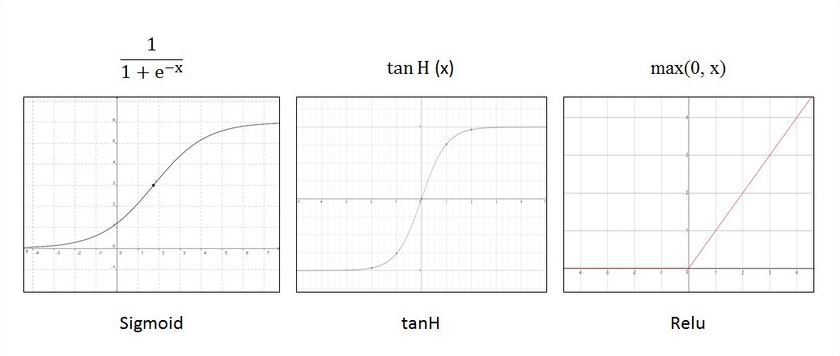
\includegraphics[width=1.0\textwidth]{./assets/img/activation_function.png}
    \caption{Figure shows the three activation functions sigmoid, tanh, and ReLu and their respective equation. Figure from \cite{haque2018image}}
    \label{fig:Activation_Functions}
\end{figure}

\noindent
% Multi-Layer Perceptron
Following the invention of the perceptron, researchers began to stack multiple perceptrons in layers and interconnect these layers.\
In this arrangement, the outputs of perceptrons in one layer serve as inputs to perceptrons in the next layer.\
This architecture is commonly known as a \gls{mlp}, as shown in Figure \ref{fig:MLP-Visualisation}.
\newline
\newline
The \gls{mlp} shown in Figure \ref{fig:MLP-Visualisation} consists of four different layers ($L$ = 4).\
The first layer is referred to as the \textit{input layer}, while the last layer is referred to as the \textit{output layer}.\
Intermediate layers between the input and output layers are commonly referred to as \textit{hidden layers}.
\newline
\newline
These hidden layers are often referred to as \textit{fully connected layers} because every input in one layer is connected to every perceptron in the next layer.\
This connectivity results in an extensive network of interconnected weights, allowing for complex data transformations and feature extraction.

\begin{figure}[htbp]
    \centering
    \begin{tikzpicture}[]
        \def\nodedist{35pt}
        \def\layerdist{80pt}
        \def\pindist{20pt}
        
        \tikzstyle{every pin edge}=[signal]
        \tikzstyle{annot} = [text width=4em, text centered]
        
        \foreach \y in {1,...,3}
            \node[inputnode, pin={[pin edge={latex-}, pin distance=\pindist]left:Input \y}] 
                (I\y) at (0,-\y*\nodedist) {$x_\y$};  
    
        \foreach \y in {1,...,4}
            \node[hiddennode] 
                (H1\y) at ($(\layerdist,-\y*\nodedist) +(0, 0.5*\nodedist)$) {$z_\y^1$};
        
        \foreach \y in {1,...,4}
            \node[hiddennode] 
                (H2\y) at ($(2*\layerdist,-\y*\nodedist) +(0, 0.5*\nodedist)$) {$z_\y^2$};
        
        \foreach \y in {1,...,2}
            \node[outputnode, pin={[pin edge={-latex}, pin distance=\pindist]right:Output \y}]
                (O\y) at ($(H21) + (\layerdist, -\y*\nodedist)$) {$\hat{y}_\y$};
    
        \foreach \dest in {1,...,4}
            \foreach \source in {1,...,3}
                \draw[signal] (I\source) -- (H1\dest);
        
        \foreach \dest in {1,...,4}
            \foreach \source in {1,...,4}
                \draw[signal] (H1\source) -- (H2\dest);
        
        \foreach \dest in {1,...,2}
            \foreach \source in {1,...,4}
                \draw[signal] (H2\source) edge (O\dest);
    
        \node[annot, above=4pt of H11] (hl) {Hidden layer 1};
        \node[annot, above=4pt of H21] (hl) {Hidden layer 2};
        \node[annot] at (I1 |- hl) {Input layer};
        \node[annot] at (O1 |- hl) {Output layer};
    \end{tikzpicture}
    \caption[Visualisation of a multilevel perceptron]{Visualisation of a multilevel perceptron, where $z_1^1$ is one example of a single perceptron in the network}
    \label{fig:MLP-Visualisation}
\end{figure}

\noindent
% Training Process
To obtain accurate results, the \gls{nn} must learn the optimal parameters $\theta_{ij}^{(l)}$ for a given problem.\
This learning process is facilitated by a technique known as backpropagation and optimisation.\
Backpropagation is an algorithm designed to determine how well the current predictions match the desired solution by computing gradients of the loss function with respect to the network parameters.\
The first step in backpropagation is to evaluate the discrepancy between the current predictions and the desired outcome.\
This evaluation is typically based on a loss function denoted as $\mathcal{L}$ or, in some contexts, a cost function.\
For regression tasks, the mean squared error (\gls{mse}) is often used and can be calculated using the equation \ref{eq:mean_squared_error}.\
Equation \ref{eq:cross-entropy} shows the calculation for the cross-entropy loss, which is often used in classification tasks.\
Having calculated the loss, the next step is to quantify the impact of each weight $\theta_{ij}^{(l)}$ on the error incurred.\
This is done by calculating gradients of the cost function $\mathcal{L}$ relative to the weights $\theta_{ij}^{(l)}$.\

\myequations{Mean Squared Error}
\begin{equation}
    \centering
    \mathcal{L}_{\text{MSE}}(y, \hat{y}) = \frac{1}{n} \sum^n_{i=1}(y_i - \hat{y}_i)^2
    \label{eq:mean_squared_error}
\end{equation}

\myequations{Cross-Entropy}
\begin{equation}
    \centering
    \mathcal{L}_{\text{CE}}(y, \hat{y}) = - \frac{1}{n} \sum^n_{i=1}\sum^K_{k=1}y_{ik} \cdot \text{log}(\hat{y}_{ik})
    \label{eq:cross-entropy}
\end{equation}

\noindent
The gradient serves as an indicator of both direction and rate, indicating the fastest ascent.\
The equation \ref{eq:backpropagation_gradient} calculates the gradients of the cost function $\mathcal{L}$ with respect to the weights $\theta_{ij}^{(l)}$ using partial derivatives.\
This equation is particularly focused on computing the gradients of the weights coming from the last hidden layer (\textit{hidden layer 2}, e.g. $z_1^2$) shown in figure \ref{fig:MLP-Visualisation}), where $l = 2$.\
For lower layers within the network, the chain rule of differentiation becomes more complicated and needs to be applied more extensively.\
Furthermore, the same mathematical framework can be used to compute the gradients of the cost function $\mathcal{L}$ with respect to the bias terms.\
Since the cost function doesn't depend directly on the weights, the chain rule becomes an essential tool for these calculations.

\myequations{Gradient of cost function with respect to the weights}
\begin{equation}
    \centering
    \frac{\partial \mathcal{L}}{\partial\theta_{ji}^{(l)}} = \frac{\partial \mathcal{L}}{\partial\hat{y}_i}\times\frac{\partial\hat{y}_i}{\partial z^{(l)}_j}\times\frac{\partial z^{(l)}_j}{\partial\theta_{ji}^{(l)}}
    \label{eq:backpropagation_gradient}
\end{equation}

\noindent
The final step in the learning process of a \gls{nn} is optimisation.\
In the equation \ref{eq:nn_optimisation}, the weights and biases are adjusted in proportion to the negated gradient of the cost function with respect to their respective weight or bias.\
This iterative learning process is repeated until the \gls{nn} converges to either a local or global minimum.\
To maximise the changes to find a global or local minima, a learning rate $\alpha$ that controls the step size is used. The learning rate controls the step size taken during the optimisation process, thus allowing a more efficient search for the optimal solution.

\myequations{Optimisation of the weights and biases}
\begin{equation}
    \centering
    \theta_{ij}^{(l)} \leftarrow \theta_{ij}^{(l)} - \alpha \nabla \mathcal{L}\Big(\theta_{ij}^{(l)}\Big) 
    \label{eq:nn_optimisation}
\end{equation}
    
\subsection{Recurrent Neural Networks}
\label{sub:RNN}

% Introduction
In the field of \gls{nn}, a significant breakthrough emerged with the introduction of the \gls{rnn}.\
Unlike traditional feedforward \glspl{nn}, \glspl{rnn} possess the unique capability to capture dependencies among sequential inputs.\
This section explores the evolution of the \gls{rnn} and its core constituents.
\newline
\newline
The inception of the modern \gls{rnn} is credited to the contributions of several remarkable researchers.\
Among them, Wilhelm Lenz and Ernst Isings introduced the Ising model, while John Hopfield expanded upon this concept by developing the Hopfield network, drawing inspiration from Shun'ichi Amari's adaptive model of the Ising model \citep{hopfield1982neural}.\
Finally, David Rumelhart's groundbreaking work on backpropagation in 1986 further advanced the field \citep{rumelhart1986learning}.
\newline
\newline
% Building blocks
The \gls{rnn} is a type of \gls{nn} designed to process sequential data by retaining some form of memory from previous time steps.\
This feature makes it particularly well suited to tasks such as natural language processing, speech recognition and time series analysis, where current inputs depend on previous inputs.
\newline
\newline
The architecture consists of an input $x_t$, a hidden state $h_t$, a loop over the hidden state, and the output $\hat{y_t}$ at time step $t \in \mathbb{R}$, as shown in figure \ref{fig:RNN_Architecture}.\
The unfolded view illustrates that each hidden state has its own weights, biases and activation function.\
At each time step, there are two inputs to the hidden state: the output of the previous state $h_{t-1}$, and the input at that time step $x_t$.\
The former input is multiplied by a weight matrix $W^{(hh)}$ and the latter by a weight matrix $W^{(hx)}$ to produce output features $h_t$, which are multiplied by a weight matrix $W^{(s)}$ and run through an activation function $\sigma$ to produce the prediction output $\hat{y}_t$.
\newline
\newline
The equation \ref{eq:update_hidden_state} computes the hidden state output at each time step.\
The equation \ref{eq:calculating_the_output} can then be used to calculate the prediction output at each time step by feeding in the weight matrix multiplied by the hidden state output and then passing it through an activation function $f(\cdot)$.

\myequations{Computing the next hidden state}
\begin{equation}
    \centering
    h_t = \sigma \Big( W^{(hh)}h_{t-1} + W^{(hx)}x_t \Big)
    \label{eq:update_hidden_state}
\end{equation}

\myequations{Calculating the output prediction}
\begin{equation}
    \centering
    \hat{y}_t = f\Big( W^{(s)}h_{t} \Big)
    \label{eq:calculating_the_output}
\end{equation}

\begin{figure}[ht]
    \centering
    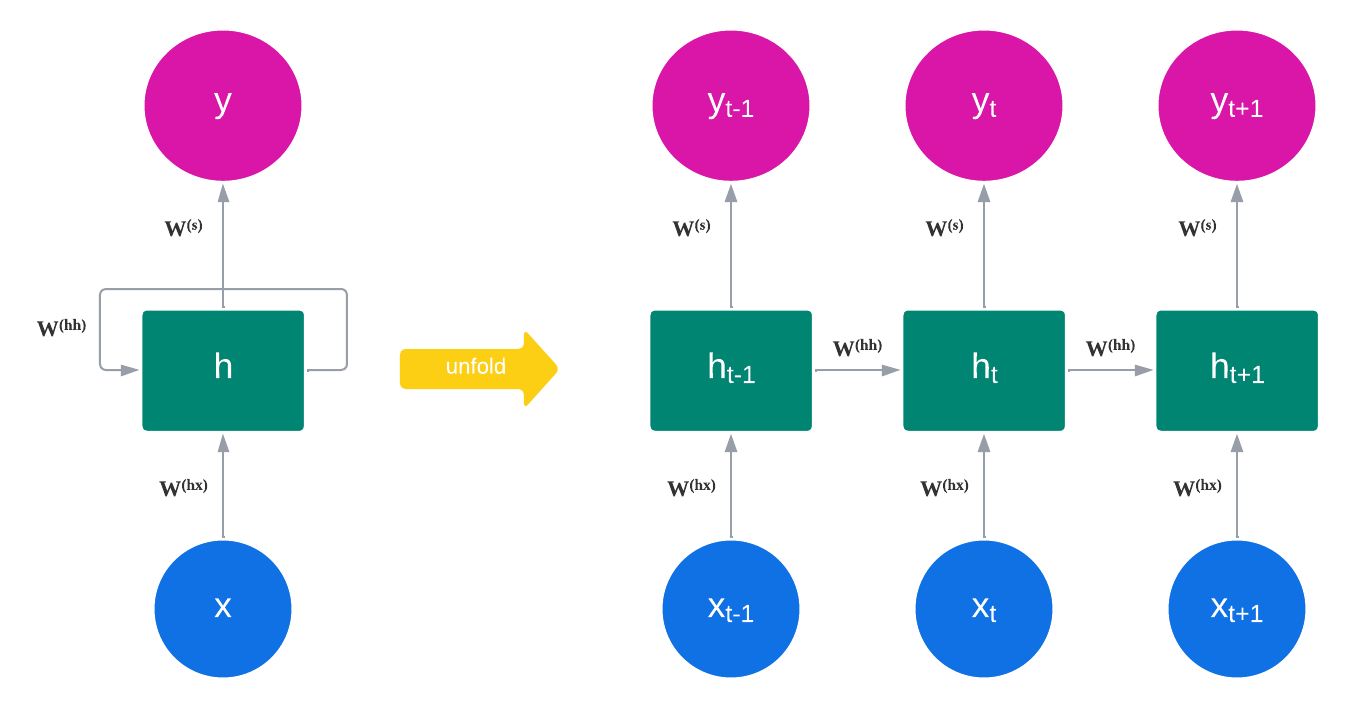
\includegraphics[width=0.75\textwidth]{./assets/img/architecture_rnn.png}
    \caption{Illustration of the folded and unfolded \gls{rnn} architecture.}
    \label{fig:RNN_Architecture}
\end{figure}

\noindent
As the same weights $W^{hh}$ and $W^{hx}$ are applied repeatedly at each time step.\
The number of parameters the model has to learn is less and, most importantly, independent of the length of the input sequence, thus defeating the curse of dimensionality.
\newline
\newline
% Training process
The training process of a \gls{rnn} is similar to that of a feedforward \gls{nn}. However, it introduces the added complexity of dealing with sequential data, where the primary objective remains the same: to minimise the calculated loss $J(\theta)$ by computing the gradients with respect to the parameters $W^{(hx)}$, $W^{(hh)}$, and $W^{(s)}$, and iteratively adjusting these parameters until they reach their optimal values.
\newline
\newline
To achieve this goal, the \gls{rnn} uses a specialised learning technique known as \gls{bptt}. Unlike traditional backpropagation used in feedforward networks, \gls{bptt} is designed to take into account the temporal nature of sequential data, making it well suited for sequential data processing. This concept was originally introduced by Werbos in 1990 \citep{werbos1990backpropagation}.
\newline
\newline
The equation \ref{eq:bptt} calculates the gradients of $J(\theta)$ with respect to $W^{(hh)}$. Since $W^{(hh)}$ is utilized in every time step up to the current output, the algorithm must backpropagate gradients from time step $t$ all the way back to initial time step $t = 0$. Once these gradients have been computed, the model parameters can be updated using equation \ref{eq:rnn_weight_update}.

\myequations{Backpropagation Through Time}
\begin{equation}
    \centering
    \frac{\partial J^{(t)}}{\partial W^{(hh)}} = \sum_{i=0}^t \frac{\partial J^{(t)}}{\partial \hat{y}^{(t)}} \cdot \frac{\partial \hat{y}^{(t)}}{\partial h_{t}} \cdot \frac{\partial h_{t}}{\partial h_{i}} \cdot \frac{\partial h_{i}}{\partial W^{(hh)}}
    \label{eq:bptt}
\end{equation}

\myequations{Updating RNN Parameters}
\begin{equation}
    \centering
    W^{(hh)} = W^{(hh)} - \alpha \cdot \frac{\partial J}{\partial W}^{(hh)}
    \label{eq:rnn_weight_update}
\end{equation}

\noindent
However, the challenge arises from the dependence of \gls{bptt} on $\frac{\partial h_t}{\partial h_i}$, which is itself a chain rule, as shown in the equation \ref{eq:unfold_chain_rule}. This leads to the vanishing gradient problem, where gradients can become progressively smaller and approach values close to zero. This happens when gradients are initially less than one and are repeatedly multiplied by gradients from earlier time steps, as shown in equation \ref{eq:vanishing_gradient_problem}. As a result, these gradients become extremely small, rendering them ineffective for parameter updates. This limitation hinders the network's ability to capture long-range dependencies in the data.

\myequations{Unfold of the chain rule for hidden state 3 to 1}
\begin{equation}
    \centering
    \frac{\partial h^{(3)}}{\partial h^{(1)}} = \frac{\partial h_{3}}{\partial h^{2}} \cdot \frac{\partial h_{2}}{\partial h^{1}}
    \label{eq:unfold_chain_rule}
\end{equation}

\myequations{Vanishing Gradient Problem}
\begin{equation}
    \centering
    \frac{\partial J^{(t)}}{\partial W^{(hh)}} = \sum_{i=0}^t \frac{\partial J^{(t)}}{\partial \hat{y}^{(t)}} \cdot \frac{\partial \hat{y}^{(t)}}{\partial h_{t}} \cdot
    \left(\prod_{j=i+1}^t \frac{\partial h_j}{\partial h_{j-1}} \right)
    \cdot
    \frac{\partial h_{i}}{\partial W^{(hh)}}
    \label{eq:vanishing_gradient_problem}
\end{equation}

\noindent
Various techniques have been developed to address the challenge of vanishing gradients, including the introduction of advanced \gls{rnn} architectures such as the \gls{lstm} network.

\subsection{Long Short-Term Memory}
\label{sub:LSTM}

% Introduction
In 1997, Hochreiter and Schmidhuber introduced a model known as \gls{lstm}. This model addresses the vanishing gradient problem within \glspl{rnn} by incorporating gated activation functions \citep{hochreiter1997long}.
\newline
\newline
% Building blocks
\glspl{lstm} are designed to enhance the memory persistence of \glspl{rnn}, making it easier for them to capture long-term dependencies. All \glspl{rnn} consist of a chain of repeating neural network modules. In standard \glspl{rnn}, these modules are relatively simple, often having only a single \gls{tanh} activation function, as shown in Figure \ref{fig:repeating_modules_rnn}.

\begin{figure}[ht]
    \centering
    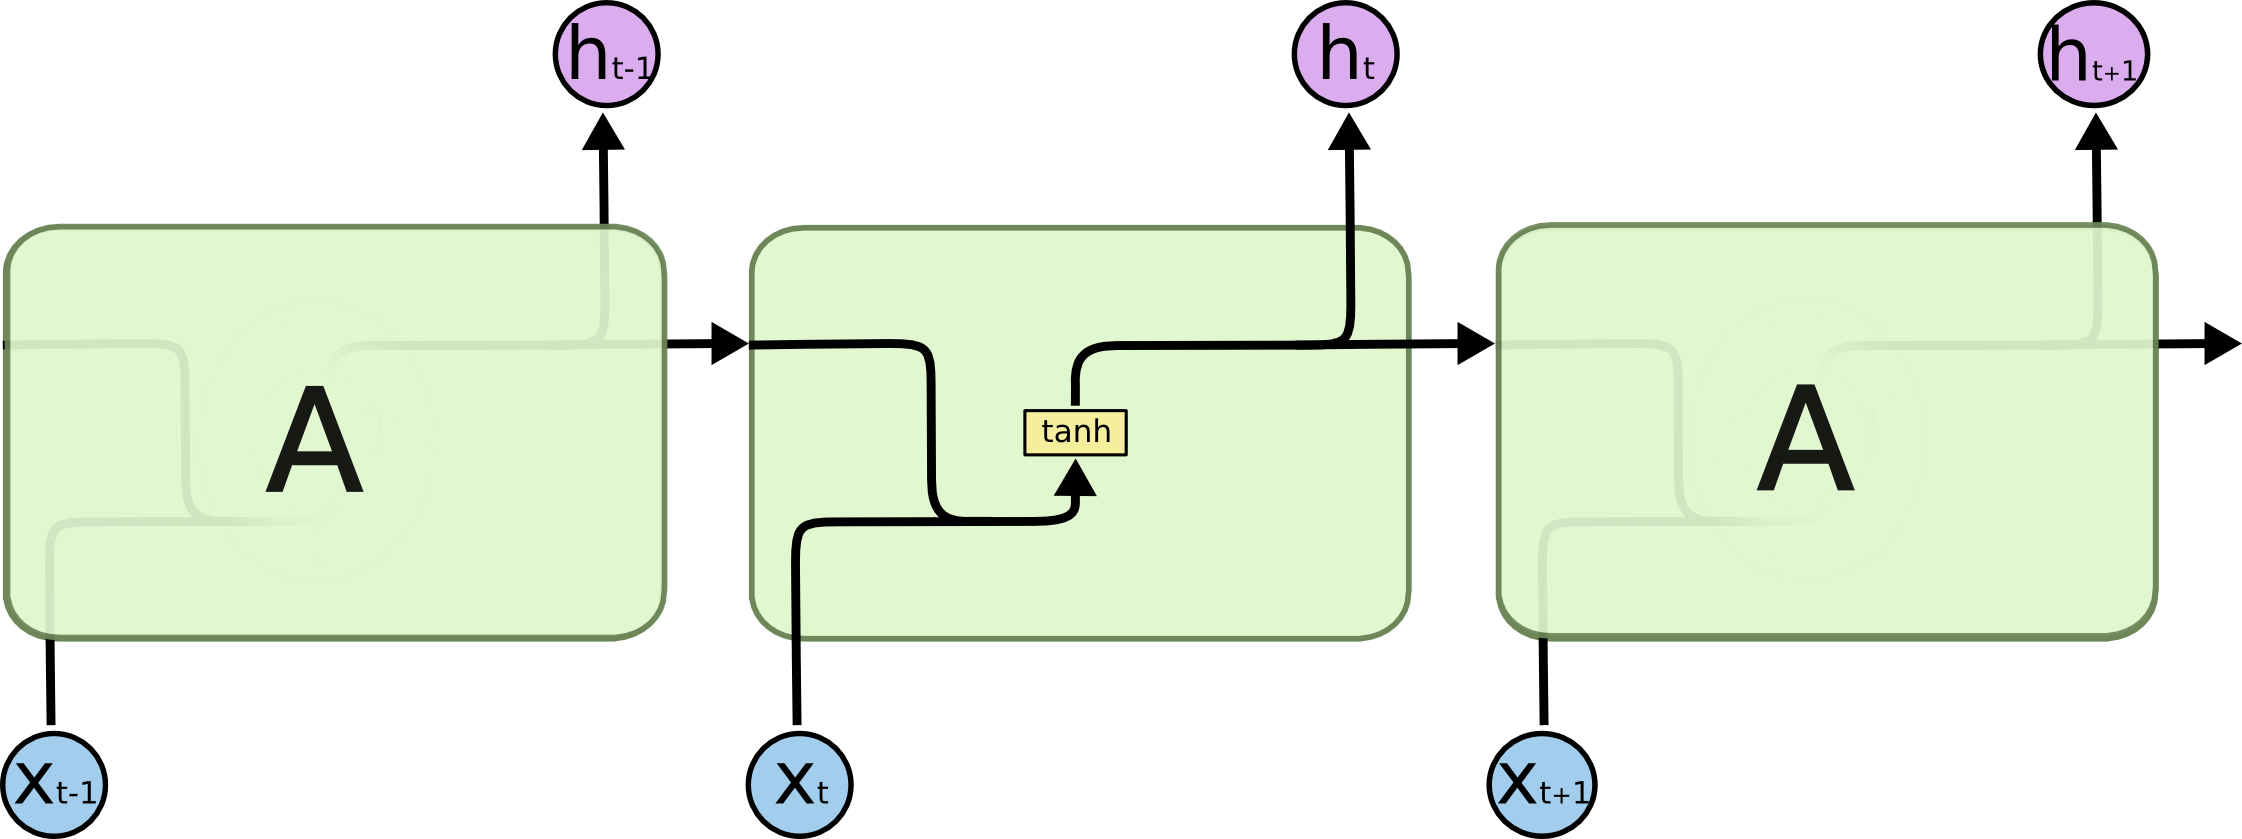
\includegraphics[width=0.75\textwidth]{./assets/img/repeating_modules_rnn.png}
    \caption{The repeating module in a standard \gls{rnn} contains a single layer. Figure from \cite{Olah_2015}.}
    \label{fig:repeating_modules_rnn}
\end{figure}

\noindent
In contrast, \glspl{lstm} also use a chain-like structure, but their repeating module is more complicated. Instead of a single layer, it consists of four interconnected layers, as shown in figure \ref{fig:repeating_modules_lstm}.

\begin{figure}[ht]
    \centering
    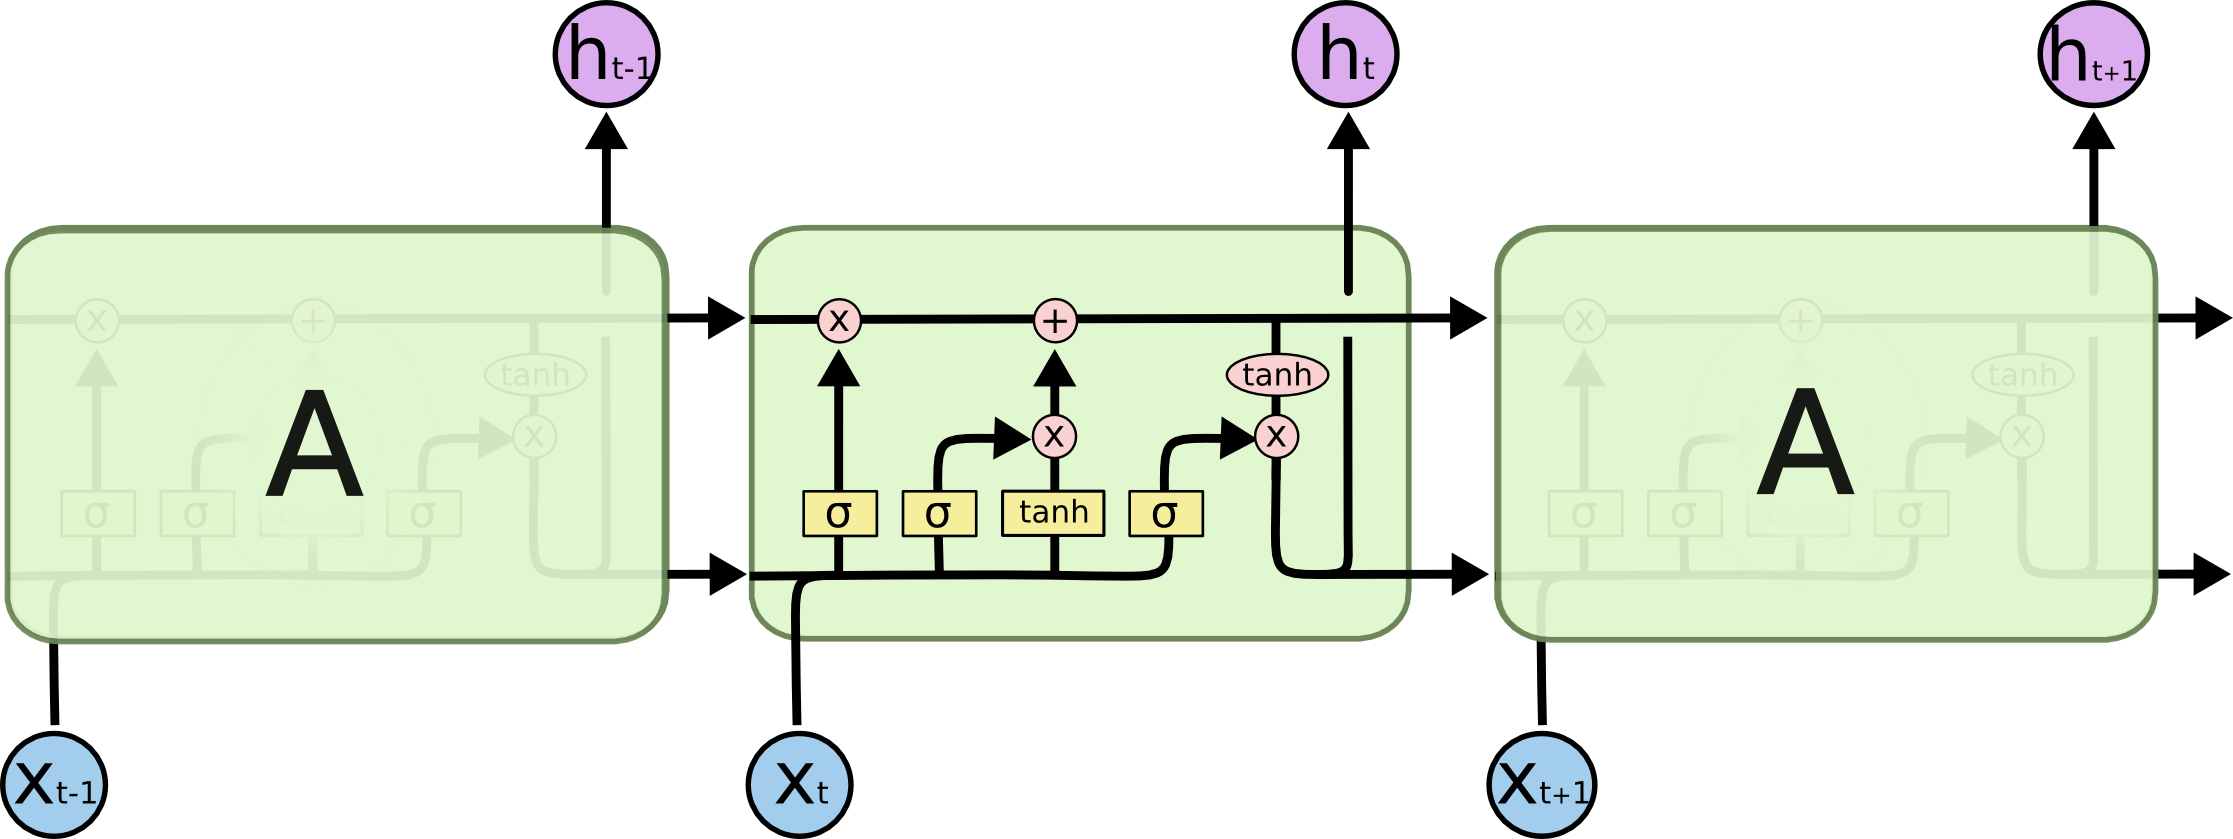
\includegraphics[width=0.75\textwidth]{./assets/img/repeating_modules_lstm.png}
    \caption{The repeating module in a \gls{lstm} contains four interacting layers. Figure from \cite{Olah_2015}.}
    \label{fig:repeating_modules_lstm}
\end{figure}

\noindent
The heart of \glspl{lstm} is the \textit{cell state}, a horizontal line that runs from the left to the right top of the diagram in figure \ref{fig:cell_state_lstm}.

\begin{figure}[ht]
    \centering
    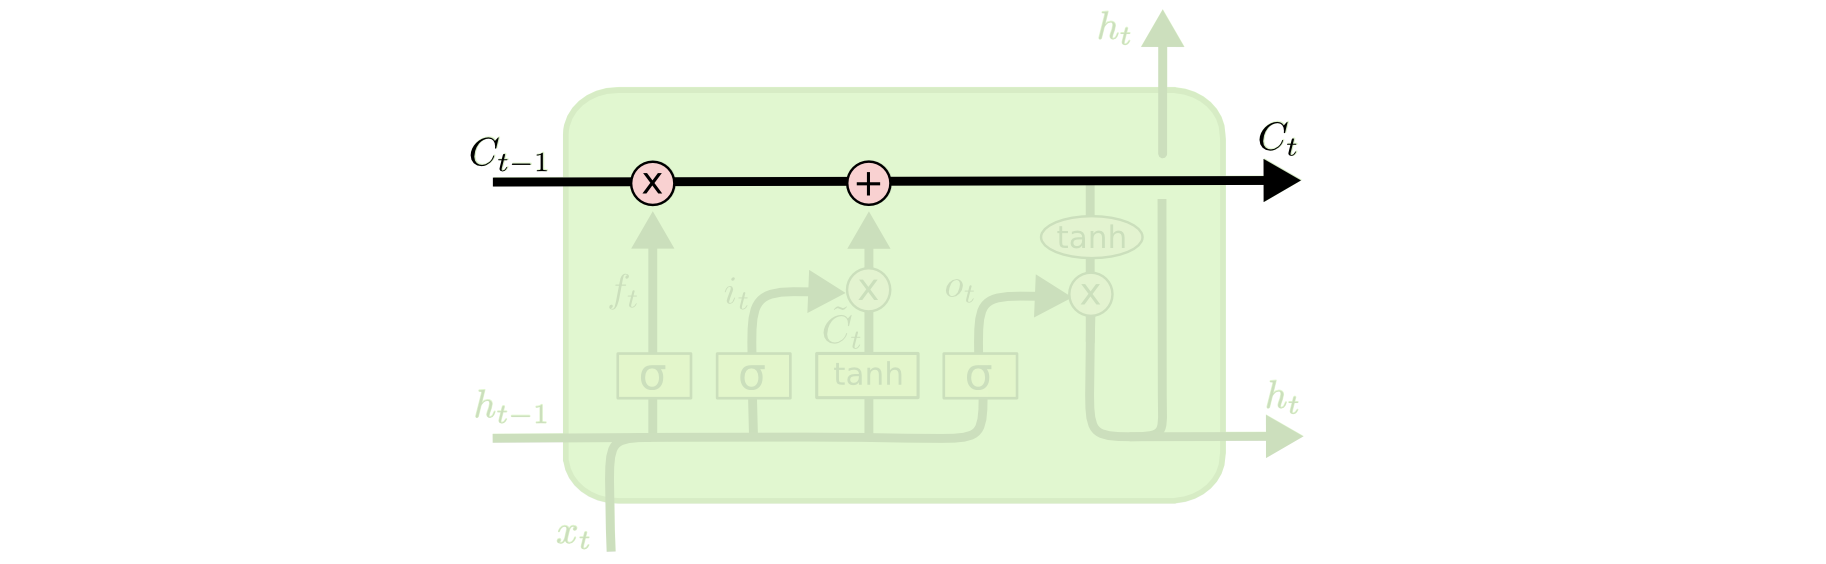
\includegraphics[width=0.85\textwidth]{./assets/img/cell_state_lstm.png}
    \caption{Cell state in \glspl{lstm}. Figure from \cite{Olah_2015}.}
    \label{fig:cell_state_lstm}
\end{figure}

\noindent
The \textit{cell state} runs along the entire chain, allowing information to flow relatively unchanged. The unique feature of the \gls{lstm} network is its ability to selectively remove or add information to the \textit{cell state}, a process controlled by specialised structures called \textit{gates}. \textit{Gates} act as filters, determining which information should pass through. They consist of a sigmoid neural network layer and pointwise multiplication, as illustrated in figure \ref{fig:gates_of_lstms}.

\begin{figure}[ht]
    \centering
    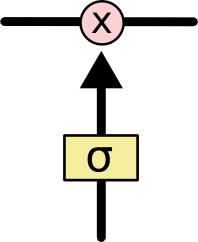
\includegraphics[keepaspectratio,height=3cm]{./assets/img/gates_of_lstms.png}
    \caption{Gates of \glspl{lstm}. Figure from \cite{Olah_2015}.}
    \label{fig:gates_of_lstms}
\end{figure}

\noindent
The sigmoid layer outputs values between zero and one, indicating how much of each component should pass, and can be calculated using the equation from figure \ref{fig:Activation_Functions}. A value of zero implies no information transfer, while a value of one allows everything to pass. \glspl{lstm} integrates three such gates, as shown in figure \ref{fig:lstm_gates}, to control and manage the state of the cell.

\begin{figure}[htb]
    \centering
    \begin{subfigure}{.45\linewidth}
        \centering
        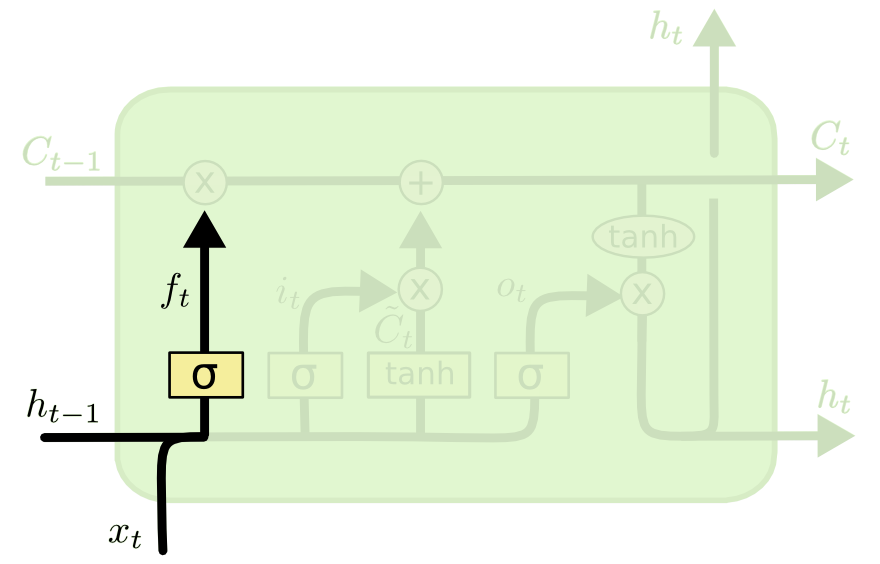
\includegraphics[width=1.0\linewidth]{./assets/img/forget_gate.png}
        \caption{Forget Gate}
        \label{fig:lstm_forget_gate}
    \end{subfigure}
        \begin{subfigure}{.45\linewidth}
        \centering
        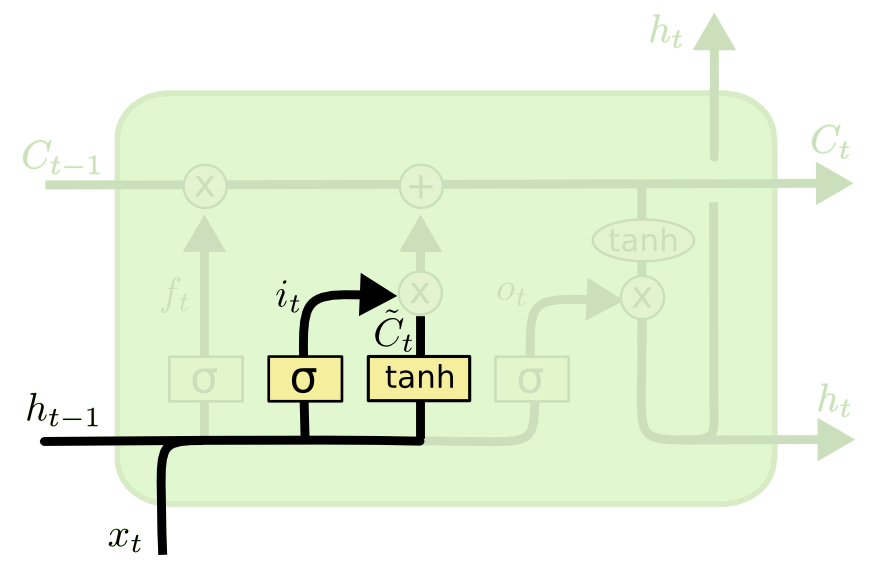
\includegraphics[width=1.0\linewidth]{./assets/img/input_gate.png}
        \caption{Input Gate}
        \label{fig:lstm_input_gate}
    \end{subfigure}
        \begin{subfigure}{.45\linewidth}
        \centering
        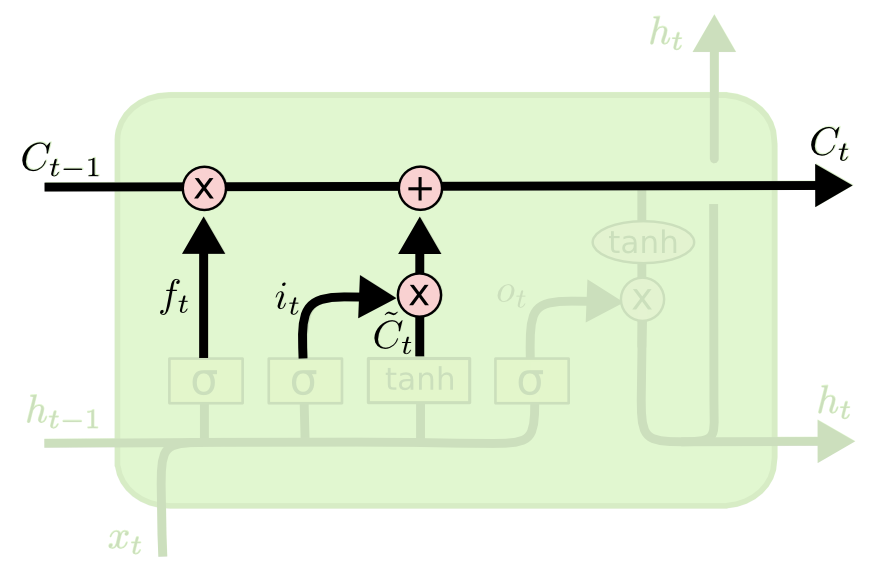
\includegraphics[width=1.0\linewidth]{./assets/img/update_gate.png}
        \caption{Update Gate}
        \label{fig:lstm_update_gate}
    \end{subfigure}
        \begin{subfigure}{.45\linewidth}
        \centering
        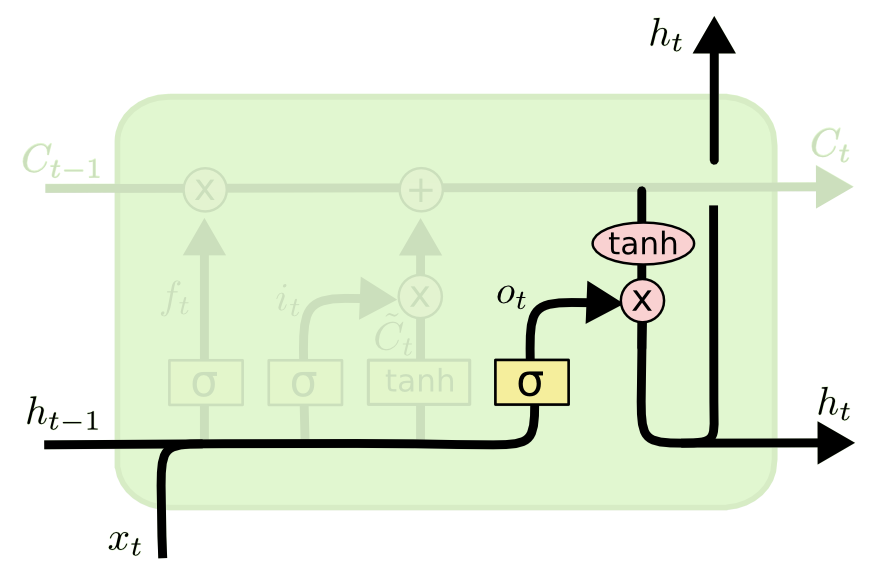
\includegraphics[width=1.0\linewidth]{./assets/img/output_gate.png}
        \caption{Output Gate}
        \label{fig:lstm_output_gate}
    \end{subfigure}
    \caption{The four \gls{lstm} gates. Figure from \cite{Olah_2015}}
    \label{fig:lstm_gates}
\end{figure}

\noindent
% Gates step-by-step
The first gate, known as the \textit{forget gate} (figure \ref{fig:lstm_forget_gate}), determines which information in the cell state should be discarded. It calculates the output using the equation \ref{eq:calculation_forget_gate}.

\myequations{Calculating the output of the forget gate}
\begin{equation}
    \centering
    f_t = \sigma \left(W_f \cdot [h_{t-1}, x_t] + b_f \right)
    \label{eq:calculation_forget_gate}
\end{equation}

\noindent
The second gate, the \textit{input gate} (figure \ref{fig:lstm_input_gate}), controls the addition of new information to the \textit{cell state}. This gate has two parts: the first, a sigmoid layer called the \textit{input gate layer}, determines which values to update, as shown in equation \ref{eq:input_gate}. Next, a \gls{tanh} layer generates a vector of new candidate values ($\tilde{C}_t$) that could be incorporated into the state, according to the equation \ref{eq:candidates_cell_state}.

\myequations{Calculating the decision of new inputs}
\begin{equation}
    \centering
    i_t = \sigma \left(W_i \cdot [h_{t-1}, x_t] + b_i \right)
    \label{eq:input_gate}
\end{equation}

\myequations{Calculating the candidates for the cell state}
\begin{equation}
    \centering
    \tilde{C}_t = \text{tanh} \left(W_C \cdot [h_{t-1}, x_t] + b_C \right)
    \label{eq:candidates_cell_state}
\end{equation}

\noindent
Subsequently, the \textit{update gate} (figure \ref{fig:lstm_update_gate}) modifies the old \textit{cell state} ($\tilde{C}_{t-1}$) to obtain the new \textit{cell state} ($\tilde{C}_t$) according to equation \ref{eq:update_cell_state}. It combines the effect of the forget gate (as calculated in equation \ref{eq:calculation_forget_gate}) and the decision of the input gate.

\myequations{Updating the cell state}
\begin{equation}
    \centering
    \tilde{C}_t = f_t \cdot \tilde{C}_{t-1} + i_t \cdot \tilde{C}_{t}
    \label{eq:update_cell_state}
\end{equation}

\noindent
Finally, the \textit{output gate} (figure \ref{fig:lstm_output_gate}) also has two components: the first, governed by the equation \ref{eq:output_gate_sigmoid}, calculates the information from the input that should be used, applying a sigmoid activation function. This result is then multiplied by the information from the cell state passing through a \gls{tanh} layer, as shown in equation \ref{eq:output_gate_tanh}.

\myequations{Sigmoid activation output gate}
\begin{equation}
    \centering
    o_t = \sigma \left( W_o [h_{t-1,x_t}] + b_o \right)
    \label{eq:output_gate_sigmoid}
\end{equation}

\myequations{Updating the cell state}
\begin{equation}
    \centering
    h_t = o_t \cdot \text{tanh}(C_t)
    \label{eq:output_gate_tanh}
\end{equation}

\subsection{Activation Functions}
\label{sub:AF}

% Introduction
Activation functions play a crucial role in \gls{nn} by introducing non-linearity. Without a non-linear activation function, \glspl{nn} would be limited to learning linear relationships in the data. The choice of activation function depends on the task and the specific requirements of the model.

\subsubsection{Sigmoid}
\label{subsub:Sigmoid}
The sigmoid activation function, denoted $\sigma$, is defined by the equation \ref{eq:sigmoid}. This function scales the values to the range [0, 1], allowing a probabilistic interpretation of the output. The sigmoid function, which is often used in the last layer of binary classification problems, is continuous and differentiable. However, it suffers from vanishing gradients due to saturation regions at -$\infty$ and +$\infty$.

\myequations{Sigmoid Activation Function}
\begin{equation}
    \centering
    \sigma(z) = \frac{1}{1 + e^{-z}}
    \label{eq:sigmoid}
\end{equation}

\subsubsection{Softmax}
\label{subsub:Softmax}
The softmax activation function, a generalisation of the sigmoid for multiple mutually exclusive classes, is given by the equation \ref{eq:softmax}. When there is only one class, the softmax and sigmoid functions are equivalent. Typically used as the final activation function in \glspl{nn}, softmax normalises the network output to a probability distribution over the predicted classes. It ensures that the output components fall within [0, 1] and sum to 1, allowing interpretation as a probability distribution.

\myequations{Softmax Activation Function}
\begin{equation}
    \centering
    \text{softmax}(z)_i = \frac{e^{z_i}}{\sum_{k=1}^K e^{z_k}}
    \label{eq:softmax}
\end{equation}

\subsubsection{Hyperbolic Tangent}
\label{subsub:Tanh}
The \gls{tanh} function, given by equation \ref{eq:tanh}, produces outputs in the range [-1, 1] centered on zero. Continuous and differentiable, tanh suffers from vanishing gradient due to saturation regions. It is a suitable choice when a zero-centred output is desired.

\myequations{tanh Activation Function}
\begin{equation}
    \centering
    \text{tanh}(z) = \frac{e^z - e^{-z}}{e^z + e^{-z}} = 2 \cdot \sigma(2z) - 1
    \label{eq:tanh}
\end{equation}

\subsubsection{Rectified Linear Unit}
\label{subsub:tanh}
\gls{relu}, defined by the equation \ref{eq:relu}, is one of the most commonly used activation functions. It replaces negative values with zero and leaves positive values unchanged.

\myequations{ReLU Activation Function}
\begin{equation}
    \centering
    \text{ReLU}(z) = \text{max}(0, z)
    \label{eq:relu}
\end{equation}
	\chapter{Methodology}
\label{ch:Methodology}
This chapter outlines the basic components used in this study, including the dataset and models. The models are implemented in Python 3.9.4 and \gls{wandb} is used for dataset versioning, experimental tracking and hyperparameter tuning.

\section{Dataset}
\label{sec:Data_Set}
This thesis aims to evaluate the performance of a machine learning approach using historical price and volume data of \gls{btc} compared to a simple buy-and-hold strategy. The dataset must therefore include historical \gls{ohlc} and volume data of \gls{btc}. In addition, a test dataset containing historical price and volume data of \gls{eth} is required to evaluate whether the model generalizes or not. 

\subsection{Data Mining}
\label{sub:Data_Mining}
The most common way to obtain historical price and volume data is to access a data provider's API. These providers can be categorized into cryptocurrency exchanges (as discussed in in section \ref{sub:Exchanges}) and general market data providers. Cryptocurrency exchanges such as Binance and Coinbase offer historical price data for various derivatives listed on their platform via their API. General market data providers such as CoinGecko and CoinMarketCap aggregate data from multiple sources to provide a comprehensive view of the market. This comprehensive data collection can then also be accessed via their API. Liu et al. for example collected price and volume data for 3703 cryptocurrencies in 2023 using CoinMarketCap \citep{liu2023forecasting}.
\newline
\newline
It's worth noting that many providers require subscription-based access to their API. Due to budget constraints, alternative sources such as investing.com have to be used. Investing.com aggregates data for 8355 cryptocurrencies\footnote{https://www.investing.com/crypto/, accessed 16/10/2023}, compared to the 8898 listed on CoinMarketCap\footnote{https://coinmarketcap.com/, accessed 16/10/2023}. Historical data for a specific cryptocurrency can be manually obtained from investing.com by visiting the historical data page, selecting the desired \gls{tf} and period, and then downloading it. This simple process was done for both \gls{btc} and \gls{eth} on the daily \gls{tf}.
\newline
\newline
The resulting individual dataset is a CSV file containing the date, open, high, low, close, volume and percentage change between the previous and current daily close.

\subsection{Data Source}
\label{sub:Data_Source}
As part of any data science project, a \gls{dqa} is performed to check for data sanity. One of these checks include whether the data source is trustworthy. In this case, the data was sourced from investing.com, which in turn was sourced from the Bitfinex crypto exchange.
\newline
\newline
Basic information about Bitfinex has been researched. Founded in 2012, the first available data point for \gls{btc} on \gls{tv} is from 31 March 2013. However, the data obtained from investing.com start on 18 July 2010. A similar patter is observed for \gls{eth}, where the first available \gls{tv} data point is from 25 June 2016 and the dataset starts on 10 March 2016.
\newline
\newline
For simplicity, all data prior to the first \gls{tv} data point are dropped for both \gls{btc} and \gls{eth}. Consequently, the \gls{btc} dataset is reduced from 4837 to 3851 data points, and the \gls{eth} dataset undergoes a similar reduction.
\section{Data Preprocessing}
\label{sec:Data_Preprocessing}
When preparing datasets for machine learning models, a critical step is to transform them into a machine-readable format, known as preprocessing. In addition, existing data is used to generate features, broadly classified into three categories ($i$) statistical, ($ii$) technical and oscillator indicators and ($iii$) the label. This section outlines the detailed transformations applied within each category.

\subsection{Data Cleaning}
\label{sub:Data_Cleaning}
In order to use the data from the data mining process (see \ref{sub:Data_Mining}) for feature generation, the data must be cleaned. In the case of this thesis, each dataset sample represents one trading day, from 00:00 to 23:59. Both datasets have common variables:

\begin{description}
    \item[Date]: Date of the sample
    \item[Price]: The price when the trading day ended
    \item[Open]: The price when the trading day started
    \item[High]: The highest price reached during the trading day
    \item[Low]: The lowest price reached during the trading day
    \item[Vol.]: is the Volume of the sample in USD
    \item[Change \%]: Percentage difference between the close of the previous and current sample, also known as the daily return
\end{description}

\noindent
The values of these variables are initially in an unreadable format, which requires the following changes:
\begin{enumerate}
    \item Drop the variable \textit{Change \%} because it is rounded to two decimal points
    \item Change variable names to lowercase and remove unnecessary punctuation
    \item Rename the variable \textit{price} to \textit{close}
    \item Change the order of the \gls{ohlc} variables to match the abbreviation
    \item Convert the variable \textit{date} to the standardised datetime format
    \item Convert the values of the \gls{ohlc} variables to the datatype float
    \item Convert the variable \textit{vol} first to the datatype integer and then into the log format
    \item Sort the dataset in ascending order and reset the index
\end{enumerate}

\subsection{Feature Engineering}
\label{sub:Feature_Engineering}
The cleaned dataset contains the variables \textit{date}, \textit{open}, \textit{high}, \textit{low}, \textit{close}, \textit{vol} in a computer readable format. Additional statistical and technical indicators (see section \ref{sec:TechnicalIndicators}) can be derived from these variables. The feature engineering in this thesis is divided into two sections: statistical indicators and technical indicators.

\subsubsection{Statistical Indicators}
\label{subsub:Statistical_Indicators}
From the variable \textit{close}, \gls{p1dr}, \gls{p7dr} and \gls{p30dr} are calculated. These returns, which are stationary and normally distributed, offer advantages over the non-stationary \textit{close} variable. In addition, the returns are transformed into logarithmic format, which makes them additive. Finally, the \gls{std} and skewness of the \gls{p1dr} over the last 30 days are calculated according to \cite{liu2023forecasting}.

\subsubsection{Technical Indicators}
\label{subsub:Technical_Indicators}
In addition to the statistical indicators, several technical indicators commonly used in technical analysis are calculated. These include several \glspl{ema} (12, 26, 50, 200), the \gls{macd}, \gls{bb}, \gls{rsi}, \gls{cci}, \gls{obv}, \gls{adx} and \gls{ad}.

\subsection{Label Engineering}
\label{sub:Label_Engineering}
To train a machine learning model, a target feature, or label, must be computed. In financial asset forecasting, three commonly used methods are tomorrow's closing price, tomorrow's log \gls{p1dr}, and tomorrow's price direction. This thesis focuses on the third approach, tomorrow's price direction, because research has shown that machine learning models fail to grasp the magnitude of the close price and thus, the simplest and most straight forward method is to predict only tomorrow's price direction. TODO: better formulate this section. The issue with tomorrow's close price is that the close price is non-stationary, i.e., it is dependent of the current close price.

\subsubsection{Data Discretization}
\label{subsub:Data_Discretization}
To predict tomorrow's price direction, \gls{p1dr} is discretized into three classes: decreasing, increasing and stationary as recommended by experts \citep{attanasio2019quantitative}.

\begin{enumerate}
    \item \gls{p1dr} below -1\% is labelled as decrease (0)
    \item \gls{p1dr} above 1\% is labelled as increase (2)
    \item \gls{p1dr} in between is labelled as stationary (1)
\end{enumerate}

\noindent
The final labels are then moved back one position within the dataset.

\subsection{Versioning}
\label{sub:Versioning}
For efficient storage and reproducibility of results,  both raw and preprocessed datasets are logged using \gls{wandb}. \gls{wandb} provides not only versioning on its platform, but also the traceability of dataset usage.
\section{Experimental Setup}
\label{sec:Experimental_Setup}
This section describes the implemented supervised learning model architectures along with their input pipeline and training procedure. In addition, information about the training infrastructure is included. Chapter 4 then presents the results from the training and evaluation.

\subsection{Training Setup}
\label{sub:Training_Setup}
All experiments were conducted locally on a Macbook Air (mid 2022) equipped with 16 GB of system memory and an Apple M2 CPU with 8 cores (4 performance and 4 efficiency). To track and visualize the experiments \gls{wandb} was used, since it also offers out-of-the-box hyperparameter optimisation tools called sweeps.
\newline
\newline
For the \gls{lstm} model a single pass through the entire dataset is referred to as one epoch. After each epoch, the model performance is measured on the validation set.

\subsection{Input pipeline}
\label{sub:Input_Pipeline}
The input pipeline is a critical component in the refinement of preprocessed datasets for machine learning applications. This section outlines the specific steps taken in the input pipeline. First, a unified data loader is implemented, followed by different training approaches tailored to the two machine learning models: \gls{xgboost} and \gls{lstm}.

\subsection{Data Loader}
\label{sub:Data_Loader}
After locally preprocessing and logging the datasets on \gls{wandb}, the data loader plays a key role in the systematic management of the datasets. The process involves downloading the data from \gls{wandb} and storing it locally. The loader then splits the dataset into a train/val set and a test set. The train/val set faciliates initial model training and hyperparameter turning, while the test set contains samples not seen during training, ensuring an unbiased evaluation of model performance after the training has been completed. Hyperparameter tuning, a critical step in machine learning model optimisation, involves defining the best hyperparameters. Commonly tuned hyperparameters include the learning rate, which affects how model parameters are updated. The data loader hands further down the train/val and test set to the appropriate model input pipeline for further processing.

\subsection{Expanding Window}
\label{sub:Expanding_Window}
The \gls{xgboost} model uses an expanding window approach. In this strategy, the model is first trained on samples $x_i$ to $x_n$ $\forall i \in \{0, 1, ..., n\}$ and predicts the next sample $x_{n+1},$ evaluating the prediction against the true class by utilizing the multi-class cross-entropy loss function. The model is then retrained on samples $x_i$ to $x_{n+1}$ and continues to predict the next sample $i_{n+2}.$ This iterative process is repeated until the model predicts the final sample in the train/val data set.

\subsection{Rolling Window}
\label{sub:Rolling_Window}
In contrast, the \gls{lstm} model uses a rolling window approach. In the first iteration, the model is trained on samples $x_i$ to $x_n \forall i \in \{0, 1, ..., n\}$ and predicts sample $x_{n+1}.$ The model is then retrained on samples $i_1$ to $i_{n+1}$ and predicts the following sample $i_{n+2}.$ This method ensures that the model consistently processes the same number of samples in a sequence during each training step.

\subsection{Models}
\label{sec:Models}
As already outlined in section \ref{sub:Input_Pipeline}, the two machine learning models used in this thesis are \gls{xgboost} and \gls{lstm}. This section describes the implementation details of the two supervised machine learning algorithms.

\subsubsection{\gls{xgboost}}
\label{subsub:XGBoost_train}
The proposed \gls{xgboost} algorihtm in \cite{liu2023forecasting} was implemented according to the paper with the default configurations. However, the paper implements the \gls{xgboost} for a regression task and uses the $R^2$ as loss function. This thesis implements the algorithm for a classification task and thus, the multi-class cross entropy loss function is used. The code was implemented using the official dmlc XGBoost library\footnote{https://xgboost.readthedocs.io/en/latest/index.html, accessed on 14.11.2023}. The models hyperparameter were tuned using the multi-class cross entropy loss, and the weighted F1 score. The model was trained using the best hyperparameters from the hyperparamter tuning. The final hyperparameters, as well as the tested one, are given in table.

\subsubsection{\gls{lstm}}
\label{subsub:LSTM_train}
\cite{yadav2020optimizing} conducted experiments on the optimization of the \gls{lstm} algorithm for time series prediction in the Indian stock market. Thus, the algorithm was implemented using the configurations of the best performing \gls{lstm} model. As already noted previously for the \gls{xgboost} model, the same problem with the loss function arises. \citep{yadav2020optimizing} also trained the model to solve a regression task and used the \gls{mse} for the loss function. This was adapted to the classifcation task at hand. In contrast to the \gls{xgboost} model the categorical cross entropy loss function was implemented. Since the two algorithms differently update their model parameters. The models hyperparameter were tuned using the validation scores and the weighted F1 scores. The model was trained using Adam without any learning rate scheduler. The final hyperparameters, as well as the tested ones, are given in table.
\section{Metrics}
\label{sec:Metrics}
Meaningful metrics need to be used to evaluate and compare the performance of machine learning models. 


\subsection{Model Performance}
\label{sub:Model_Performance}
A often used metric for classification tasks is the calculation of the F1 score, which is the harmonic mean between the precision and the recall. However, this metric does not take into account the fact that in a trading strategy not all true positives and prediction errors have the same importance. Thus, a custom weighted F1 score is implemented according to \cite{wang2018financial}. The metric differentiate between three types of errors. The first error $E_{1st}$ is when the model predicts either an increase or decrease in price, but the true class yields the opposite. The second error $E_{2nd}$ is when the model predicts either an increase or decrease in price, but the true value is flat. And finally, the third error $E_{3rd}$ is when the model predicts flat but the true value is either an increase or decrease. In addition, not all true positives have the same importance as well. This is the case when the price stays flat. Thus, the above mentioned errors $E_{2nd}$ and $E_{3rd}$ as well as the true positive for flat predictions are penalized with a constant $\beta^2$, to give more importance to the true positives in either increase or decrease and the first error $E_{1st}$. In the case of this thesis, the constants for $\beta^2$ are 0.25 for $\beta_1^2$ and 0.125 for $\beta_2^2$ and $\beta_3^2$.

\myequations{Compute variables for Weighted F1 score}
\begin{equation}
    \centering
    N_{tp} = N_{ti} + N_{td} + \beta_3^2 N_{tf}
    E_{1st} = E_{witd} + E_{wdti}
    E_{2nd} = E_{witf} + E_{wdtf}
    E_{3rd} = E_{wfti} + E_{wftd}
    \label{eq:compute_variables_f1}
\end{equation}

\myequations{Compute Weighted F1 score}
\begin{equation}
    \centering
    F = \frac{(1+\beta_1^2+\beta_2^2) N_{tp}}{(1+\beta_1^2 + \beta_2^2) N_{tp} + E_{1st} + \beta_1^2 E_{2nd} + \beta_2^2 E_{3rd}}
    \label{eq:compute_weighted_f1}
\end{equation}

\subsection{Portfolio Performance}
\label{sub:Portfolio_Performance}
To measure the performance of the model on the portfolio level the metrics turnover, number of trades, statistics about the \gls{pnl} and the max drawdown are calculated.
\section{Backtesting}
\label{sec:Backtesting}
In order to assess the predictive performance of the machine learning models, a so-called baseline has to be established first. In the case of this thesis, three common used trading strategies from the domain of algorithmic trading are used. Namely, a sma-based strategy, a momentum based strategy and a mean reversion strategy. It is important to note, that these strategies only take long positions, as the drawdawn for short positions can be 100\% of the invested capital and cryptocurrencies are extremly volatile, leading to a complete loss of funds in the worst case. In addition, to trade perps usually margin has to be deposited to the exchange. Where margin is a collateral in the case of default. The margin depends on position size, restrictions by the exchange and the amount of leverage used. For the purpose of this thesis, the later is not being further discussed. If trades are executed without leverage, the margin is equivalent to the position size. For example, a \gls{btc} short position is opened at \$19'000, but the price rises instead of falling, ending at \$40'000. Latest at \$38'000 the position got liquidated because the position was in 100\% loss and thus, the exchange automatically closed the position. In reality there are funding fees, which are necessary to keep perps pegged to the underlying asset and thus, the position would have been liquidated already before \$38'000.
Note that the start value of the trading account is in all events set to 10'000 USD.

\subsection{Baselines}
\label{sub:Baselines}
Lorem Ipsum

\subsubsection{SMA-based Trading Strategy}
\label{subsub:BB_Baseline}
 The baseline that uses the \gls{bb} as signals for positions, executes a long position when the daily close price is below or equal to the $\text{BOLD}$. The position will be closed when the close price is above or at the $\text{BOLU}$. In order to create the dataset containing the results for the \gls{bb} baseline, the \gls{bb} are first calculated using the \gls{bb} method from the TA-Lib. Next, the initial account value has to be set to 10'000 USD. Finally, the positions have to be calculated and the final account value calculated.  

\subsubsection{Momentum Trading Strategy}
\label{subsub:RSI_Baseline}
Lorem Ipsum

\subsubsection{Mean Reversion Trading Strategy}
\label{sub:Global_Benchmark}
Lorem Ipsum

\subsection{Benchmark}
Lorem Ipsum	
	%\input{./parts/04_results.tex}
	%\input{./parts/05_discussion.tex}

	\appendix
	%\input{./parts/99_appendix.tex}
    
    \newpage
    \printglossary[type=\acronymtype, title=List of Abbreviations]
    \newpage
	\listoffigures
	\newpage
	\listoftables
	\newpage
	\listofalgorithms
	\newpage
	\listofmyequations
	
    \newpage
	\bibliography{references}
	\bibliographystyle{apalike}	
\end{document}